\documentclass[conference,10pt,final,letterpaper]{IEEEtran}
\usepackage[T1]{fontenc}
\usepackage{tgtermes}
\usepackage{subcaption}
\usepackage{graphicx}
\usepackage{geometry}
\usepackage{float}
\usepackage{amsmath}
\usepackage{amssymb}
\usepackage{enumitem}
\usepackage{array}
\usepackage{tabu}
\usepackage{multirow}
\usepackage{textcomp}
\usepackage{gensymb}
\usepackage{pdfpages}
	
	
%\DeclareCaptionSubType[alph]{figure}
%\captionsetup[subfigure]{labelformat=simple,justification=centerlast}

%\renewcommand\thesubfigure{(\alph{subfigure})}
%\makeatletter
%\renewcommand\p@subfigure{\thefigure}
%\makeatother

\geometry{
	a4paper, 
	total={8.5in,11in},
	left=0.5in,
	right=0.5in,
	top=0.5in,
	bottom=0.5in,
}
%\linespread{1.0}


\begin{document}

\title{Automated detection of dune crest-lines in planetary satellite images}
\author{David Leblanc, George Bebis, Mircea Nicolescu, Nicholas Lancaster}

\IEEEtitleabstractindextext{%
\begin{abstract}
Dune-field patterns are believed to behave as self-organizing systems, but what causes the patterns to form is still poorly understood. The most obvious (and in many cases the most significant) aspect of a dune system is the pattern of dune crest lines. Extracting meaningful features such as crest length, orientation, spacing, bifurcations, and merging of crests from image data can reveal important information about the specific dune-field morphological properties, development, and response to changes in boundary conditions. However manual methods are labor-intensive and time-consuming. 

In this research, we are developing the capability automatically detect crest-lines and computing the geomorphological properties of dune fields, using satellite images on planetary surfaces. Our goal is to develop a robust methodology and the necessary algorithms for automated or semi-automated extraction of dune morphometric information from image data.

We investigated multiple different approaches to solve the problem, ranging from appearance-based, gradient-based, and machine learning methods. We strive to solve the problem caused by the inherent bimodal distribution of the histogram of the gradients by computing the overall dominant orientation of the dune field gradients. The concept of the gradient direction map is also introduced as a method to segment areas of the image which agree with the dominant orientation of the dune fields. Crest-line candidates can be extracted from the segmented areas which are in turn filtered using the responses of a train machine learning model. Once candidate crest-lines have been detected, the morphological properties of the dune field can be computed.

Our approach has been tested on two distinct dataset including satellite images of six terrestrial regions and from Mars. The results reported perform well on both linear and complex dune structures, and have relatively high precision and recall rates and low error in computation of the morphological properties, indicating that our approach generally robust.
\end{abstract}

% Note that keywords are not normally used for peerreview papers.
\begin{IEEEkeywords}
	
\end{IEEEkeywords}}


\maketitle

\IEEEdisplaynontitleabstractindextext

\IEEEpeerreviewmaketitle

%%%%%%%%%%%%%%%%%%%%%%%%%%%%%%%%%%%%%%%%%%%%%%%%%%
\pagenumbering{arabic}
%%% Body of Manuscript %%%%%%%%%%%%%%%%%%%%%%%%%%%

\section{Introduction}

Computer vision, image understanding, and machine learning are fields that have been thriving in the last few decades with advances in computing. The purpose of these are to extract information and understanding from images and various types of data. Many disciplines use the techniques to solve specific and challenging problems. Humans are typically good at recognizing and understanding these problems \cite{statistical-pattern-recognition}, but the work required to apply the solution can be either complex or tedious.

Along with the challenges and complexity associated with the problems is the data collection process. Technological advancements in the ability to capture, record, and store data from many different sources has provided increasingly large data sets which need processing. The amount of data is overwhelming for humans to manually process, therefore the need for automated solutions becomes even more significant.

In this research, the goal is to create an automated system able to analyze and extract geomorphological properties from satellite images of dunes by extracting dune crest-lines. Dune fields and crest-lines have various morphological properties which includes dune type, size, height, width, length, orientation, spacing or wavelength. In past research, the properties were measured manually by experts in the field using \emph{Geographic Information Systems} (GIS) applications \cite{ewing-kocurek-lake-2006,ewing-peyret-kocurek-bourke-2010,fenton-michaels-beyer-2014,fenton-michaels-chojnacki-beyer-2014,kocurek-ewing-2005}. \emph{Digital Elevation Maps} (DEM) have grown in popularity in recent years. DEM planetary data sets for Earth (e.g. SRTM, ASTER, GDEM, and other high resolution data sets), Mars (HiRISE, MOC), and Titan (Cassini radar) are now available and provides information on many of the aeolian bedform morphology, orientations, and dune types of each region. Therefore, a need for an automated, or semi-automated processing method and statistical analysis of the dune patterns has arisen.

Our research will focus on developing a automated system to extract, recognize, and characterize dune patterns on images of planetary surfaces. The requirements are that the application robustly and automatically (or perhaps semi-automatically) detects crest-lines from various dune morphological types, such as linear, complex, or other types. Additionally, the ability to automatically compute the dune properties such as crest length, orientation, and spacing could greatly benefit and provide a valuable tool for the research community.

The research done in \cite{ewing-kocurek-lake-2006,ewing-peyret-kocurek-bourke-2010} shows that dune patterns can be characterized using the following metrics:
\begin{enumerate}
	\item Trend or Orientation of dunes
	\item Crest lengths of dunes
	\item Dune spacing or wavelength
	\item Defect density (breaks in the pattern, terminations, forks, bifurcations, etc) per unit length of the dune crest-line, used as a measure of the degree of organization of the field.
\end{enumerate}

The metrics above are illustrated in Figure \ref{fig:dune_pattern_metrics}. These metrics are important properties which characterize the dune field, and enable researchers to deduct meaningful information about the particular regions. Ideally, any algorithm which processes the data should correctly and clearly identify crest-lines, characterize the dune types, and extract the metrics described above.

\begin{figure}
	\centering
	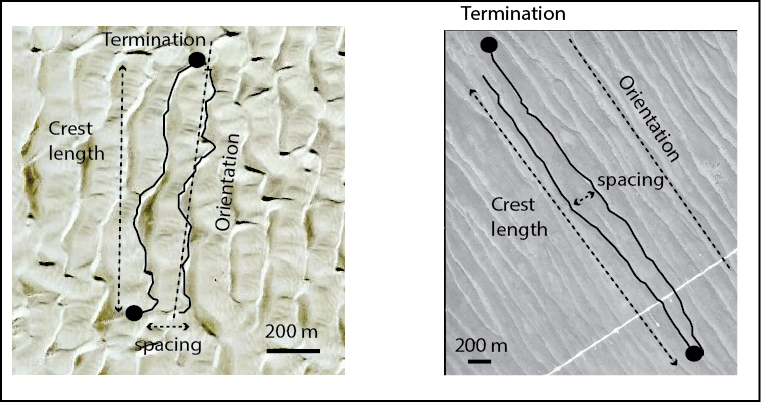
\includegraphics[width=\linewidth]{figures/dune_pattern_analysis}
	\caption{Examples of dune pattern analysis including metrics such as orientation, crest length, spacing, and termination points.}
	\label{fig:dune_pattern_metrics}
\end{figure}

\subsection{Challenges}

In order to automatically compute the metrics, the dune crest-lines must first be correctly detected and identified. Therefore, the bulk of the research presented will focus on crest-line detection, along with some general metrics calculations. Crest-lines can be defined as series of linear or curved segments, where all points along the segments represent the dune ridge line, and the ends of the segments represent the termination or defects in the pattern.

There are many ways to represent crest-lines. The most basic representation could be a vector which holds the trend or orientation (azimuth) and length. This representation is simplistic and can provide a general overview of the dune field. Sets of linear segments also facilitate the computation of some of the metrics desired. However, there are issues associated with the linear segments representation.

\begin{enumerate}
	\item Linear segments are only an approximate representation of the dune field and therefore there will be localization errors. In addition, dune crests are not always straight lines.
	\item The process of determining which linear segments are part of the actual crest-line can be difficult since there may be many false positives present in a given image.
	\item The data itself is quite noisy which will lead to many false positives in the detections.
	\item Computing accurate geomorphological metrics becomes challenging.
\end{enumerate}

A better representation would be a contiguous and smooth vector of two dimensional points which plot a curved segment, with the first and last points representing the location of the termination points. This is the representation which is favored and will be used as part of this research. The contiguous segment representation also provides a more accurate localization of dune crest-lines, and should produce more exact dune metric calculations.

Other challenges with automated crest-line detection are the algorithms and image processing tasks applied to the data sets. In satellite images of dune fields, the sun's orientation with respect to the image source greatly determines the appearance of the dunes. From an image representation perspective, a dune appears to have both a sunlit side, and a shaded side, as shown in Figure \ref{fig:intro_sample_images}. This translates to bright regions (large pixel values) for sunlit areas, and darker regions (low pixel values) for shaded areas. Crest-lines, or dune ridges, can the be defined to be the edge segments where the bright areas meet the darker areas in the image.

\begin{figure}
	\centering
	\begin{subfigure}{0.45\textwidth}
		\centering
		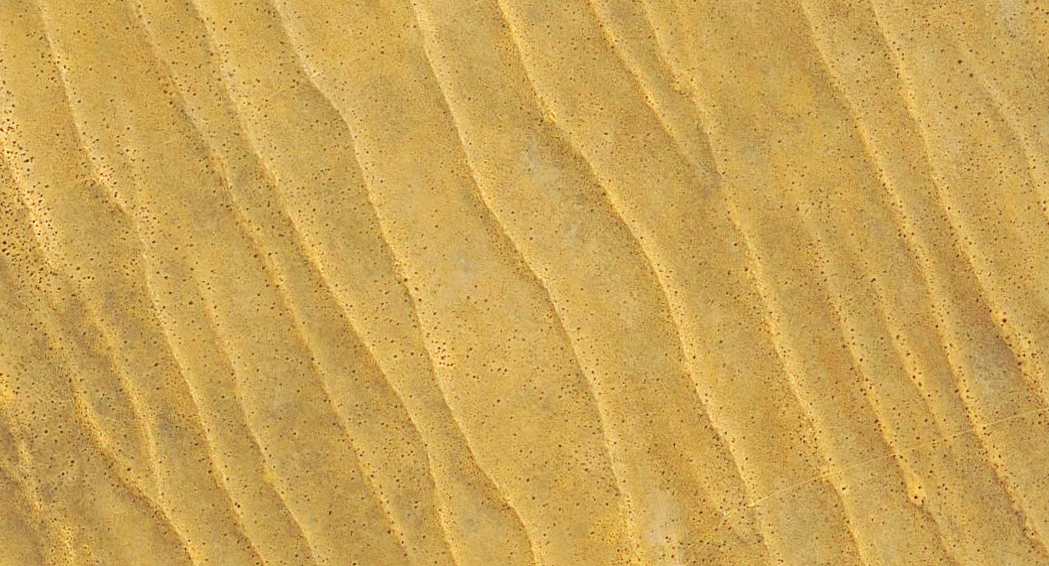
\includegraphics[width=\linewidth]{figures/kalahari}
		\caption{ Kalahari }
		\label{fig:intro_kalahari_image}
	\end{subfigure}
	\begin{subfigure}{0.45\textwidth}
		\centering
		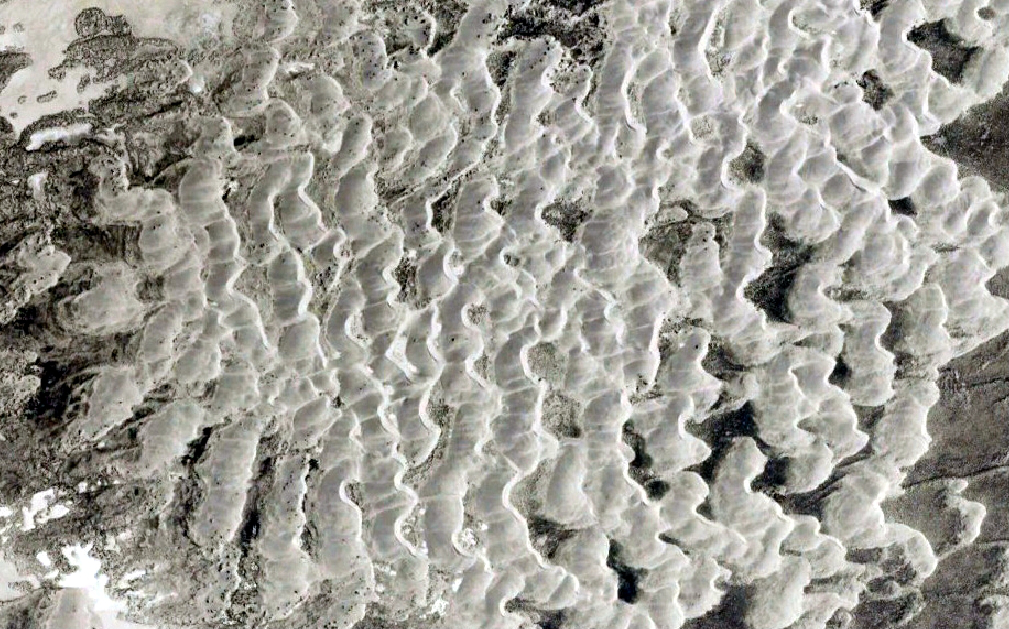
\includegraphics[width=\linewidth]{figures/wdc}
		\caption{ Winnemucca Dune Complex }
		\label{fig:intro_wdc_image}
	\end{subfigure}
	\caption{Sample satellite images of two distinct dune field regions: Kalahari and  Winnemucca Dune Complex }
	\label{fig:intro_sample_images}
\end{figure}

Issues arise when the sun's orientation is unknown, namely determining if an edge belongs to a crest-line ridge or is in fact a valley or the edge of a shadow. If the sun's orientation relative to the image is known, determining which edges are crest-lines or valleys becomes a much easier task. However, working under the assumption that the sun's relative orientation is unknown (which is the assumption made in this research), the ambiguity requires a resolution. In some cases, such as the Kalahari dune field shown in Figure \ref{fig:intro_kalahari_image}, determining the sun's orientation can be inferred from the image itself, since the dune ridges are relatively linear and well defined. On the other hand, in areas like the Winnemucca Dune Complex or WDC, shown in Figure \ref{fig:intro_wdc_image}, the sun's orientation cannot easily be determined. The factors which determine which edges are the crest-lines are not obvious, even for a human.

Another complexity which much be accounted for are the computer vision algorithms chosen to detect crest-lines. There are generally two approaches to solve these types of problems: appearance based and machine learning based approaches. Appearance-based approaches are typically fine tuned algorithms designed specifically to solve a problem set. The main drawback of these techniques are that they require significant manual tuning of parameters to achieve the desired accuracy to solve the problem. On the other hand, machine learning methods learn the problem set by example, and typically require many less parameters, which can be self optimized. Unfortunately, machine learning typically require a data set of training examples to construct the model to solve the problem. In this research, we explore both approaches using many different kinds of methods, specifically applied to the dune crest-line detection problem.

Once the crest-lines have been identified, the final challenge is computing the geomorphological properties of the dune fields. There are many levels of detail which can be computed for the metrics. At a coarse level, the global properties can be averaged for the entire dune field, while at a finer grain level, the metrics can be computed in local areas of the dune field around each crest-line. The latter is obviously more desirable, but requires more extensive and complex computations to accurately compute the desired metrics.

\subsection{Contributions}

The main contribution of this research is the development of a method to detect crest-lines from satellite images of planetary dune fields. The bulk of the research focuses on various regions on Earth, and the Ganges Chasma on Mars, also used in \cite{vaz_object_based_dune_analysis}. Each regions contains a data set of manually labeled satellite images, which includes all ground truth crest-lines.

A variety of methods were applied on each image set, and evaluated using the ground truth. Both appearance-based methods and machine learning are used to extract the crest-lines. The appearance-based method use a plethora of features such as intensity values, gradients, and frequency domain analysis, and other general image processing to attempt to find crest-lines. Machine learning methods are also used to construct models which can identify crest-line structures in the image. Each method is evaluated using the labeled ground truth, where the quality of each method is measured by precision and recall of the detected crest-lines, and the accuracy of the geomorphological metrics calculations. Each method has its own strengths and weaknesses, therefore the final proposed method combines both the edge-based and machine learning methods. 

The gradients in the image play an important role in discerning crest-lines. A critical piece of the algorithm is determining the dominant orientation of the dune field which is the overall trend of the dunes. It can be computed from the gradients of the crest-lines, which are affected by the sun's orientation relative to the dune field. 

Determining which gradients belong the the crest-lines and valleys is a challenging problem. A few solutions are proposed to solve this problem, including unsupervised methods such as K-Means, and normalized histograms of gradients. Once the dominant orientation gradients for crest-lines have been determined, the crest-lines can be more easily identified by keeping all gradients which \emph{agree} with the overall dominant orientation gradient.

Another important contribution is the \emph{gradient orientation map}. This maps the dot product of the gradients at each pixel with the computed dominant orientation gradient. In essence, pixels which \emph{agree} with the dominant orientation are emphasized separating shaded and bright sides of the dunes, which allows crest-lines to be easily traced.

The final proposed solution combines the dominant orientation, gradient orientation map, and a machine learning response map to find the crest-lines. The gradient based approach is used to extract initial candidate crest-lines. The response map is then used to both improve the localization of the crest-lines and to filter out false positive candidates.

A method for computing the dune field morphology metrics is also proposed. The main metrics computed are the overall orientation of the crest-lines, and the spacing between the crest-lines. The orientation is computed after crest-lines have been detected, which is done by quantizing the detected crest-lines into linear segments and computing the orientation of the lines. The dune spacing is computed by measuring the orthogonal distance between the lines.

The research is split into the following sections: the previous work and background is presented in section \ref{sec:background_perious_work}, which presents an overview of the study of dune fields, and work done in the field of image processing and computer vision, and previous dune detection implementations. In section \ref{sec:methodology}, the methodology is presented, included the various methods tried both for appearance-based, edge-based, and machine learning methods. It also presents the method for computing the geomorphological properties of a dune field. Section \ref{sec:experimental_evaluation} presents the  datasets used and the results of the detection and metrics for each approach. Finally, section \ref{sec:conclusion} discusses the methods and their results, along with proposing some future work on improving the approaches. 
\section{Background and Previous Work} \label{sec:background_perious_work}

In this section, the previous work done in this application is reviewed. The need for dune crest-line detection has risen recently due to many research applications in this field. Therefore, understanding the concepts and properties of dune fields is important. Section \ref{subsec:dune_pattern_studies} will present an overview of some of the research done in this field. Section \ref{subsec:image_processing_cv} will discuss some of the related algorithms and methods for processing images and computer vision used in this research. Finally, section \ref{subsec:dune_detection} will present the state of the art dune detection research which uses both appearance-based and machine learning approaches.

\subsection{Dune Pattern Studies} \label{subsec:dune_pattern_studies}

Many studies have been done on the topic of dune fields, with the ultimate goal of understanding how dunes form, behave, and which factors contribute to the systems. In \cite{Kocurek_Ewing}, an explanation of how dune-field patterns emerge is proposed and the degree of complexity from the standpoint of self-organizing system is discussed. Dune patterns are classified into two basic categories: simple or complex. According to this paper, a simple pattern is defined as having a single pattern type. Complex patterns are said to potentially have multiple spatially superimposed pattern types. Simple patterns trend towards a better ordering, so long as the wind regime remains constant. Changes in the trend of wind pattern will cause reorientation. Complex patterns can then be interpreted as the superposition of many generations of wind regimes.

Complexity can be measured using pattern analysis, measuring parameters such as the crest length, orientation, spacing,	defect density, and other properties. These properties would be very useful information to extract for the dune detection. Finding crest-lines	can help us identify the patterns, extracting meaningful data such as junctions, terminations, mergers, linking, and other interesting processes explained in \cite{Kocurek_Ewing}.

In later work, \cite{Ewing_Peyret_Kocurek_Bourke} studied the dune field pattern formations on the north polar region of Mars. These dunes are thought to be mostly inactive, with relatively no movement over a period of 4 to 15 Martian years. The reason this region is interesting is because there are two nearly orthogonal crest-line orientations present in the region. This complex system of superposition of multiple patterns in this example showcases a set of \emph{primary} and \emph{secondary} crest-lines which would be valuable data to automatically segment. The \emph{primary}	dunes are the largest-scale dunes, extend over the entire length of the image set, and contain many \emph{Y} junctions, an indication of well-organized linear dunes. In contrast, \emph{secondary} dunes are rounded, have less defined features, and are perpendicular to the main primary crest-lines.

Other interesting features are the so-called \emph{Slipfaces}. These typically appear along the \emph{primary} crest-lines, in areas of intersection with the \emph{primary} and \emph{secondary} crest-lines. Another feature are the \emph{Wind Ripples}. The ripples are present on the surface of most dunes with the exception	of \emph{slipfaces}. To detect	these types of features, a higher resolution image is a required, as those types of features are very small compared to the scale of the \emph{primary} and \emph{secondary}	dunes. \emph{Interdune Areas} are features specific to the area studied in \cite{Ewing_Peyret_Kocurek_Bourke},	have a polygonal shape, and are indicative of ice.

The rest of the paper describes an in depth statistical analysis of the features to compute the flow fields and understand the geomorphic relationships which are present in the area. The paper \cite{Ewing_Peyret_Kocurek_Bourke} provides a lot of interesting and valuable information which can be used to understand the application of automatic dune detection. If these features can be extracted, it would be interesting to see if we can do a similar statistical analysis based on the results presented. The next step would be to retrieve the HiRISE dataset and their data or ground truth to compare.

In the most recent work, \cite{Multi_spatial_analysis_aeolian_dune_field_patterns} study the aeolian dune-fields at different scales. Scale is an important factor to consider because aeolian dune-fields patterns can vary over	a wide range of scales, both spatially and temporally. Being able to measure the change of scale over time is important in order to investigate the environmental conditions of the studied region. Aeolian	dunes are developed typically in transitions from sand patches, to proto-dunes, to dunes, to dune-field patterns. Complex dune patterns are usually a juxtaposition of simple dune patterns are multiple scales. To summarize, being able to detect the crest-lines and other types of features at multiple scales is invaluable.

In other related work, \cite{Application_spatial_cross_correlation_detection_submarine_dunes} studied the migration of submarine sand dunes. The dataset used in this paper includes digital terrain models (DTMs) retrieved from high-density multibeam echosounders (MBES) taken of submarine sand dunes along the coast of New Brunswick. In order to measure the migration of these types of dunes, the motion was measured by simply subtracting the DTMs from sequences over time. The implementation uses a simple cross-correlation to find similarities from one set to the next. From the correlation matches found, the migration vector can be computed. The migration data processing can extract the flow fields of the dunes.

The research presented above is only a subset of the work done, but provides very valuable information on how, why, and what dunes are. The next section will describe some of the state-of-the-art technology in the field of image processing and computer vision. 
 
\subsection{Image Processing and Computer Vision} \label{subsec:image_processing_cv}

The main goal of image processing is to enhance and improve the quality of images in order to improve the performance of feature extraction. Computer vision is a field in which information is extracted from images for the purpose of understanding the image to solve a problem for a given application.

\subsubsection{Preprocessing}

For this application, the satellite images of the dune fields need to be processed using various known processing methods. Filtering out noise in images is critical to extracting good crest-line candidates. There are many common filtering approaches used in image processing and computer vision applications. In this application, satellite images of sand dunes may include various amounts of noise. In order to improve the dune detection algorithms, the goal of filtering is to filter out the noise while preserving or enhancing the necessary features such as the crest-line edges. In \cite{Bilateral-filtering-gray-color-images}, the bilateral filter is proposed, which allows flat noisy regions to be filtered while preserving strong edges. Bilateral filtering	is a simple non-iterative algorithm for filtering out noise.

Another key process is to normalize the illumination of the dune fields. Illumination normalization is a process in which the image illumination is made to be more evenly distributed across the image, to make the illumination invariant in conditions of varying lighting. This processing is most commonly used in face detection or recognition applications. In \cite{Illumination_normalization_based_on_2d_gaussian_model}, a Gaussian illumination model is used to stretch the contrasts of darker areas. The process involves using a Quadtree method to divide the image into sub regions to find dark areas. The areas that meet these requirements are processed with the Gaussian illumination model to brighten them up, which evens out the illumination. Applying this normalization significantly improves performance of face recognition.

In a similar approach \cite{Illumination_normalization_for_image_restoration_using_modified_retinex_algorithm}, the authors use a modified retinex algorithm to restore poorly illuminated areas of an image. According to Lambertian reflectance theory, images consist of two components, reflectance and illumination. If an image contains a set of small scale features, and large scale features, and illumination is only applied to the large-scale set, then the small scale features can be preserved. In this approach, the normalization is applied to small-scale and large-scale features independently. The Single Scale Retinex process is applied to the image to separate	the reflectance (small scale) and illumination (large scale). After, images are thresholded and histogram equalization is applied, which spreads out intensity values of darker areas of the image.

In a remote sensing application, \cite{Illumination_normalization_among_multiple_remote_senging_images}, illumination normalization is carried out in the gradient domain and using singular value equalization. According to the authors, the gradient domain image enhancement process can compress the dynamic range of images, increase contrast, and enhance fine details in darker regions. The goal of singular value equalization (SVE) is to make all images in a specific set to have similar mean intensity value. Some images may have a lower or higher mean intensity. By using SVE, the pixels can be processed to achieve a mean closer to the target intensity, therefore normalizing illumination accross a set of images. The drawback of this method is that multiple images of the same or similar scenes are required. Many of these techniques can be applied directly to processing the satellite images of the dune fields in order to improve and normalize the illumination.

Another critical processing step is to extract edges from the images. Edges are extracted by taking the derivative of an image, and preserving the strongest gradients. There are many operators used to extract edges. The Canny edge detector, first introduced in \cite{1986_canny_edge_detection}, is a well known and used method to retrieve important edge features from an image. This famous detector is often used because of it's qualities in detecting edges. The Canny edge detector typically produces a binary image of thin, contiguous, and well defined edge segments which makes it a good candidate solution for edge extraction. 

In \cite{Canny_edge_detection_enhancement_scale_multiplication}, enhancement to the method is proposed by analyzing the responses of detection at two scales. The benefits of this technique are better localization in images with larger amounts of noise, at the cost of a slightly lower detection rate. Overall the performance of the Canny operator is improved by using multiple scales.

The Canny detector is further improved in \cite{Runway_detection_tracking_unmanned} for a runway detection application for unmanned aerial vehicles. The main contribution of this paper is the use the Canny operator combined with a mean filter, and using the Hough Transform to track runways. The advantages of the mean filtering is that it filters out noise, preserves edges (better than a traditional Gaussian filter), and makes the image less fuzzy. To solve the problem of the dual threshold of the Canny operator, the proposed method is to compute the thresholds dynamically based on averages.

In \cite{Improved_Canny_Edge_Detection}, an improved implementation of the popular Canny edge detector is proposed. According to the authors, the traditional Canny algorithm suffers from two main	problems: the gradient calculation is sensitive to noise and the use of the fixed double threshold may not be suitable for images with high gradient variability. The main flaw in the gradient calculation has to do with the inequality of the edge detection in darker versus brighter regions. For the parameter selection of the double threshold, the paper propose choosing the high and low thresholds from the computed mean and standard deviation of the gradient magnitudes.

Another problem with edge detection methods can be the discontinuity of edges. The goal is often to link edges which may suffer from noisy conditions in order to produce smoother contiguous segments. In \cite{Edge_linking_using_geodesic_distance_neighborhood_information}, an edge linking approach is proposed which using local neighborhood, using geodesic distance (as opposed to the common Euclidean distance measure) between edge candidates. When calculating the direction of edge end points, typically eight directions are used, which introduces error. To address this, \cite{Edge_linking_using_geodesic_distance_neighborhood_information} define a windows size based on the maximum allowable edge gap, and fit a line to the edges, which allows a full range of directions to be accounted for. The geodesic distance measurement is not only based on euclidean distance but also on the intensity values of the image, which reportedly gives better results.

\subsubsection{Feature Detection}

Once edges have been detected, the next logical step is to extract information from the edges. In previous work, in order to detect dune crest-lines, the edges needed to be organized into line segments so geomorphological properties can be computed. Computing the orientation and dune spacing of the dune field on the satellite images requires an algorithm that can accurately detect line segments present in an image.

Line detection is a well known and challenging problem in the field of computer vision. Traditional approaches such the Hough Transform presented in \cite{1972_hough_transform_line_detect}, use edge detectors such as the Canny to extract line segments. Unfortunately, choosing the correct parameter and an appropriate threshold for preserving true positives while eliminating false positives for any task can be difficult. Inappropriate selection of the parameters causes inaccurate results in the computation of the geomorphological properties. Improvements on the technique proposed in \cite{1986_extracting_straight_lines} and \cite{2000_meaningful_alignments} improve the results slightly but basically suffer from the same parameter selection problems.

An interesting alternative to the classical Hough transform is presented in \cite{Automated_cable_tracking_sonar_imagery} in an application inspection or maintenance of underwater cable components. The paper discusses image processing techniques to extract linear features in cluttered and noisy images. After applying some anisotropic filtering to remote high frequency noise, edges and lines are detected on the sonar based images. To detect potential linear features, they use a Phase Congruency detector. The Hough transform is then used to find linear features, and a criteria is determined to reject false positives and preserve true positives.

Another promising approach to line segment detection is presented in \cite{2010_lsd_fast_line_segment_detector} which combines the features of the techniques presented above. In this approach, adjacent edge points are group by orientation, and lines are fitted to the local support region. Validation of line segments is applied using a threshold of the number of points which support the given line. The benefits of this approach is the ability to detect line segments in complex structures using minimal parameter selection. 

\begin{figure}
	\centering
	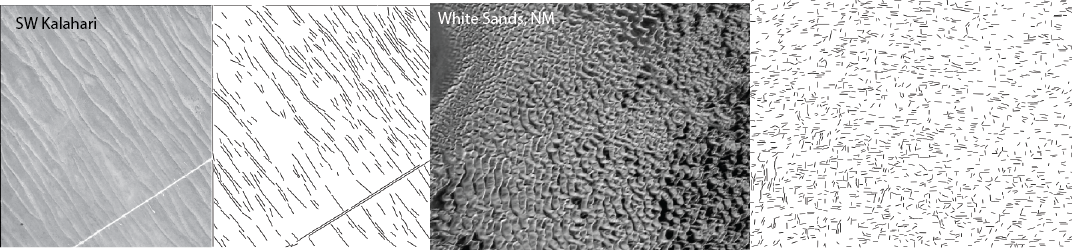
\includegraphics[width=\linewidth]{figures/lsd_results}
	\caption{Preliminary results of the Line Segment Detector (LSD \cite{2010_lsd_fast_line_segment_detector}) applied to the linear dunes of the Kalahari (left) and transverse dunes in White Sands (right). The results of the LSD on linear dunes are good, while complex transverse dune results are poor.}
	\label{fig:lsd_results}
\end{figure}

Some preliminary work was done testing the Line Segment Detector (LSD) on some dune field images, shown in Figure \ref{fig:lsd_results}. The method seemed to perform quite well on linear dune formations found in regions like the Kalahari, but performance was quite poor on regions with non-linear complex or transverse dune formations, such as the White Sands dune field.

A line detection and image enhancement has also been proposed in \cite{Robust_Faint_Line_Detection_Enhancement_Algorithm}, for a digital image restoration of heritage artwork. The images worked with have been deteriorated over time, and contain many cracks, faint lines, and broken stroke. The goal of this is to remove unwanted edges, and enhance the desired edges. The approach is implemented in three basic steps: Initial line detection with non-maxima suppression, true line detection using anisotropic refinement, and noise reduction. The initial step is to perform correlation convolving the image with some sort of edge detecting mask, rotated at different orientations, and retrieving the maximum response for the orientation	for each pixel. The paper claims this produces a sharper and more reliable edge map, which is then filtered using non-maxima suppression. This process preserves strong lines while removing texture lines. The image is the binarized to remove all remaining weak edges, and only allowing strong edges to remain. The smoothing is applied to the original based on the processing done, smoothing out weak edges, while not smoothing strong true edges.

In a similar approach, \cite{Image_Edge_detection_Rotating_Kernel_Transformation} use rotating edge detection kernels and fuse the responses from the operations. An edge is defined as a location and a direction compared to a non-edge point such as a flat area or noise, which has no specific direction. Following this principle, the response in one direction should be higher than in the other directions. For a non-edge, the	responses in each of the directions are similar. Therefore computing the mean and standard deviation of each of the kernel responses can help resolve edge versus non edge pixels. The results obtained from this process shows promising results when applied to noisy images. The approach proposed in \cite{Image_Edge_detection_Rotating_Kernel_Transformation} has definite potential for improved edge detection applied to dune crest-line detection. It also has potential for improvement of the method itself.

\begin{figure}
	\centering
	\begin{subfigure}{0.35\textwidth}
		\centering
		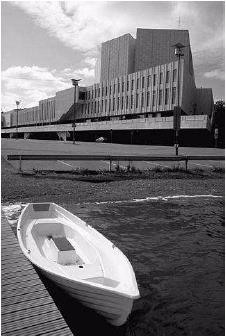
\includegraphics[width=\linewidth]{figures/tensor_voting_input}
		\caption{ Sample Image }
		\label{fig:tensor_voting_input}
	\end{subfigure}
	\begin{subfigure}{0.35\textwidth}
		\centering
		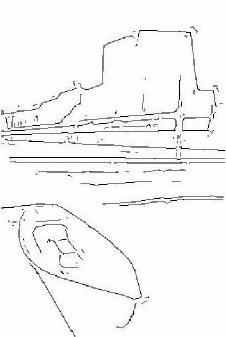
\includegraphics[width=\linewidth]{figures/tensor_voting}
		\caption{ Tensor Voting Results }
		\label{fig:tensor_voting_output}
	\end{subfigure}
	\caption{ The results of applying tensor voting schemes to find salient linear segments in an image (\cite{2009_tensor_voting_cluttered_backgrounds}) }
	\label{fig:tensor_voting_results}
\end{figure}

Tensor voting frameworks are also a potential way to extract linear segments from images, and could be useful in a dune detection application. Tensor voting has been used in various applications in computer vision such as in \cite{2006_tensor_voting_video_repairing,2005_tensor_voting_image_correction,2006_tensor_voting_stereo_monocular,2005_tensor_voting_visual_motion_analysis,2001_tensor_voting_epipolar_geometry}. One of the interesting benefits of tensor voting approaches, as explained \cite{2009_tensor_voting_cluttered_backgrounds}, is that they seem to show very good results in grouping oriented segments in highly cluttered images. The Gestalt principles of visual perception are used as the voting scheme where second order tensors are used to represent the segments. The goal is to filter out background segments while preserving the more salient segments. Figure \ref{fig:tensor_voting_results} shows the result of applying tensor voting to a sample image.

In \cite{Probabilistic-tensor-voting-robust-perceptual-grouping}, a tensor voting approach is used to perform perceptual grouping on noisy data. The approach extends the standard tensor voting using Bayesian probabilities. The Bayesian framework has added benefits of	reducing the learning variance of the perceptual grouping task. Another	contribution of this paper is the use of a 2\textsuperscript{nd} order tensor and two	types of polarity vectors to handle both outliers and inlier noise. The approach also is able to process all types of geometric structures. For probabilistic tensor voting, the voting procedure uses random vector with a given standard deviation. It uses three layers of voting:	sparse ball vote, sparse stick vote, and revised stick vote, where the goal is to change the positions of each token based on a random vector.

Another interesting approach for extracting features is segmentation. One particular method used in segmentation processes is the Watershed Transform, an approach which is used in this research and explained in section \ref{subsec:watershed_transform_segmentation_approach}. The Watershed Transform is a well known algorithm for segmenting meaningful regions from an image. The main benefit of the watershed technique as opposed to methods, such as edge-based detection, is that the watershed produces closed boundaries, which allows contours to be detected. An overview of the Watershed algorithm	is presented in \cite{Watershed-transform-definition-algorithms-parallelization-strategies}.

In \cite{Image_segmentation_using_texture_gradient_based_watershed_transform}, segmentation is achieved using the watershed transform from texture gradients. The texture gradients are retrieved using various wavelet transforms. Similarly, in \cite{Watershed-based-textural-image-segmentation}, an approach to texture segmentation is proposed. When applied to textures,	the watershed algorithm tends to over-segment a texture into small homogeneous sub-texture regions. Therefore, a texture can be determined	to be set of texture segments. The texture sub-regions can be merged using a clustering algorithm. A wavelet transform is used to characterize the irregular shaped segment regions, which are used to cluster similar	groups of sub-textures.

Another approach used in the Watershed algorithm is based on markers. The desired regions to segment can be extracted using some known feature which is marked on the image. In \cite{Fingerprint-pore-extraction-based-marker-controlled-watershed-segmentation}, this concept is applied to fingerprint pore extraction. Marker based segmentation has been shown to be robust for segmentations problems where the objects are closed contours with boundaries being ridges. In this application, the watershed transform is applied to the gradient image of the fingerprints, and the regional minimas are computed to obtain the markers, then compute the watershed transform based on the markers. In \cite{Detection-breast-tumor-candidates-using-marker-controlled-watershed-segmentation}, the watershed segmentation is applied to a breast tumor detection application. All these various researches have the potential to be useful in our dune crest-line detection application. 

Ultimately, the goal is to perform automated feature detection from satellite images. In \cite{Extraction_roads_multispectral_imagery}, a semi-automated method for extracting roads from aerial or satellite images is proposed. The purpose of this paper is to localize roads from higher resolution images, using some form of segmentation. The proposed method is semi-automated because a user must provide and initial seed point, onto which a region growing algorithm is applied to extract the road. A level set method is applied to evolve the boundary of the road region, which can better handle noise and multiple road mergers. The boundary for the desired region is based on a speed function, which is designed based on uniformity, texture, and contrast properties. Once the regions have been extracted, the centerlines of the roads are estimated using a skeletonization procedure, with junction analysis to ensure that intersections are properly handled.

In \cite{Extracting_ocean_surface_feature_modis}, linear features of internal waves are extracted using a technique called \emph{Multiscale Retinex}(MSR) feature extraction. Although the problem set in \cite{Extracting_ocean_surface_feature_modis} is different, there appears to be significant overlap and comparison between dune crest-line detection and oceanic internal wave detection. The oceanic internal waves are typically generated from many sources such as tidal currents, ocean frontal boundaries, and other atmospheric conditions. The MSR is an image processing technique that provides consistency and dynamic range compression across an image with poor contrast. The paper discusses the use both the Wavelet Transform Modulus Maxima (WTMM) and the Canny edge detector, which turned out to have superior performance.

\subsection{Dune Detection} \label{subsec:dune_detection}
The specific application of this research applies to automated detection of dune crest-lines. Some work has been done in automated dune detection. There are two main methods used to detect dune landforms and crest-lines: appearance-based and machine learning methods.

\subsubsection{Appearance-Based Methods}
In \cite{2012_automated_extraction_sand_dunes_egypt}, a Geographic Information System (GIS, \cite{gis_article}) based model is proposed and developed to study sand dune migration patterns, with the ultimate goal of predicting threats to roads, irrigation networks, water resources, urban ares, agriculture and infrastructures. Multi-temporal images of a region were collected, enhanced, and a simple image subtraction technique is used to compute the migration shift of dunes.

An automated extraction of dune features approach is proposed in \cite{2015_automated_mapping_of_linear_dunefield}, which uses the Sobel gradient operator to detect crest-lines. In this approach, the authors claim that the Canny edge detector provided poor results, and the Sobel operator generated more consistent results. The gradient magnitude of the Sobel operator is used to threshold out the weaker edges. The use of a histogram to compute the orientations of the gradients was found to have a bimodal distribution, with one of the modes being the dune edges. Dune candidates are determined based on their gradient magnitude which filter out weaker candidates unless they are near strong candidates. This research addresses the issue of determining crest-lines versus valleys or shadows, explained in section \ref{subsec:challenges}, by using the histogram of gradients. Examination of the histogram reveals that they had a strongly bimodal distribution for which one peak represents crest-lines and the other represents the valleys or shadows. The assumption made in their research is that the stronger peak represents the crest-lines, and therefore all gradients which belong to the weaker peak (within 90 degrees of the peak) are filtered out. This assumption may not always be valid, and is addressed in section \ref{subsec:edge_based_detection}.

In \cite{2016_comparisons_crest_line_extraction_marine_dunes}, an overview of various line detection algorithms are reviewed in the context of a marine dune crest-line extraction method. The research evaluates four main appearance-based approaches (\cite{2005_topology_driven_algorithms_for_ridge_extraction,2005_smooth_feature_lines_surface_meshes,2004_ridge_valley_lines_meshes_surface_fitting}) to detecting ridges from MultiBeam Echo-sounder System (MBES) data maps. The data for these approaches is essentially 3D depth maps of underwater dune forms. The challenge therefore is to trace the ridges to extract the dune crest-lines.

\subsubsection{Machine Learning Methods}
Many of the research techniques to detect and identify various landforms use commonly known machine learning techniques. In \cite{2006_automated_classification_landform_elements}, object-orientated image analysis is used to classify the type of landform elements found in Digital Terrain Models (DTM). Features such as elevation, curvature, and slope gradient are used to construct a classification model, which categorizes landform elements into nine distinct base shapes. The shapes are somewhat abstract and generalized, but the concepts presented in this paper could be applied to crest-line detection.

The research done in \cite{2007_Machine_Learning_tools_automatic_mapping_mars} developed a machine learning based approach to map and categorize various landforms on Mars. In this research, it is shown that regions can be clustered using unsupervised learning methods, and labeled using supervised learning, given a dataset which has been manually labeled. The popular Support Vector Machines classifier is used to predict the label of the clustered regions. Similar methods will be addressed in sections \ref{subsec:edge_based_detection}, \ref{subsec:machine_learning_approach}, and \ref{subsec:mixed_ml_gradient_approach}.

The research done in \cite{2013_sar_image_automated_detection_dune_area} uses a simple approach in which the correlation is computed between two images taken at different times within a year. Various window sizes are used to account for dunes of different scale. An interesting observation is made; as the window size grows larger, the correlation values tend to increase in areas where dunes are present, while remaining relatively constant in areas without dunes. A supervised learning method is used to classify areas which dunes are present.

In \cite{BandeiraMarques}, a supervised learning approach is used, training classifiers such as Support Vector Machine and Random Forests to detect dune structures on Mars. The method proposed in this paper is to classify small (40 by 40 pixels) cells in a quantized image grid. In each cell, features are computed based on the image gradients, using both phase and magnitude. In order to classify a cell as either a dune or not a dune, the features of both the cell and the cell's neighboring cells are used. The features extracted are then used to train the machine learning method, which is used to then predict if a cell is a dune.

Although this type of method has typically shown very good results, there are a few drawbacks with using supervised learning approaches. These types of methods usually require a fairly large labeled dataset which may not always be available. Anytime a dataset is constructed for this purpose, it is important to provide a large number of examples of different types of dunes, in order to get a robust representation of the problem set. In \cite{BandeiraMarques}, 230 labeled images were used to train and test the method, and have a decent representation of various dune types. Another drawback of this approach is the use of cells, for which fixed-sized cells may not be scale invariant. Also, quantizing an image into larger cells	will affect localization accuracy of the dunes. If the application requires higher localization accuracy, this type of supervised learning approach may not be suitable.

In \cite{2011_neural_network_based_dunal_landform_mapping}, texture features are extracted from images to train a multilayer perception or neural network to generate landform maps. The texture features used are the Grey Level Co-occurrence Matrix (GLCM \cite{1973_textural_features_image_classification}), are fed into the neural network with goal of characterizing various landforms. A critical problem to solve is the selection of the window size for computing the texture features. Reportedly, smaller window sizes, relative to the spatial resolution, negatively affect the classification accuracy. The window size parameter is also addressed in section \ref{subsec:machine_learning_approach}. A large dataset was used to train the neural network, and shows promising results.

The most current and direct research application to dune crest-line detection is presented in \cite{vaz_object_based_dune_analysis}. An object-based image analysis method is used to extract crest-lines from dune field datasets on mars. The main approach extracts features from the dune field images, and trains an artificial neural network classifier. Once the classifier is trained, the crest-lines can be extracted and the dune field can be analyzed. The object-based image analysis methodology is very similar to our research, and the datasets used in this paper were acquired. Section \ref{subsec:results-and-discussion} shows the comparison of the results reported in \cite{vaz_object_based_dune_analysis} and our results, using our computed dune metrics.

The remainder of this paper discusses the various methodologies (section \ref{sec:methodology}) implemented as part of this research. The approaches include both appearance-based and machine learning methods to crest-line detection. The results of each approach are then presented in section \ref{sec:experimental_evaluation}.


\section{Methodology} \label{sec:methodology}
The primary goal to reach when analyzing dune field images is to compute and extract meaningful features, as discussed in \cite{ewing-kocurek-lake-2006,ewing-peyret-kocurek-bourke-2010}. The two main features extracted in this research are the following:

 \begin{description}
 	\item [Orientation] The orientation (both local and global) of a dune field can provide researchers valuable information about climate and wind patterns in the area.
 	\item [Inter dune spacing] The distance between crest-lines also provides valuable information about structure of the dune field.
 \end{description}
 
 There are many potential methods to extract such features, but in this research, a crucial first step is to detect crest-lines in the dune field. Crest-lines are the main prominent features in any dune fields. The are characterized by a distinguishable peaks along a ridge of dunes. Extracting the dune crest-lines is a challenging problem in itself, which is explained in \ref{subsec:challenges}. In this research, a many different approaches have been attempted, which include an appearance-based approach in \ref{subsection:appearance_based_approach}, an edge-based approach in \ref{subsec:edge_based_detection}, using the Watershed Transform in \ref{subsec:watershed_transform_segmentation_approach}, a gradient orientation based method in \ref{subsec:gradient_orientation_based}, a machine learning approach in \ref{subsec:machine_learning_approach}, and ultimately the mixed gradient and machine learning approach which is explained in \ref{subsec:mixed_ml_gradient_approach}. Finally, the computation of the dune field morphology metrics is explained in section \ref{subsec:dune-field-metrics}.
 
 \subsection{Challenges} \label{subsec:challenges}
 
 Automated detection of crest-lines from satellite images poses many problems. Finding and labeling crest-lines in images in most cases may be a straight forward task for an expert researcher in this field, but quickly becomes a tedious task as the amount of data increases. The need for automated detection of such features is very apparent. However, there are regions where dune fields are complex and dense, making automated dune detection a much more difficult task.
 
 Generally, a crest-line is visible by the fact that it has a sunlit side, and a shaded side. Areas in the image where a bright region meets with a darker region are typically good candidates for potential crest-lines. In Figure \ref{fig:dune_cross_section}, a cross-section of a sample dune ridge illustrates the effects of the sun's orientation on the illumination of the dune field.
 
 \begin{figure}
 	\centering
 	%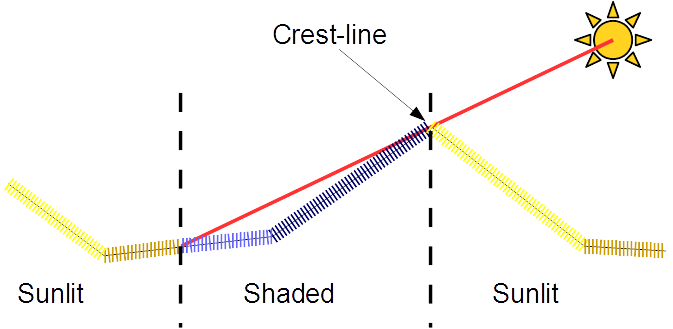
\includegraphics[width=0.75\textwidth]{figures/dune_cross_section}
 	\caption{Cross-section of a dune slope with the sun's orientation effect on shaded and sunlit portions of the dune.}
 	\label{fig:dune_cross_section}
 \end{figure}
 
 This important criteria assumes that the sun's orientation is roughly perpendicular to the dune ridges. When ridges approach a parallel orientation to the sun's orientation, the crest-lines become less pronounced. The problem is evident as shown in Figure \ref{fig:difference_between_dune_field_types}, from linear dunes in the Kalarahi (\ref{fig:difference_between_dune_field_types_kalahari}) to the complex structure of the White Sands dune field (\ref{fig:difference_between_dune_field_types_whitesands}).
 
 \begin{figure}
 	\centering
 	\begin{subfigure}{0.48\textwidth}
 		\centering
 		%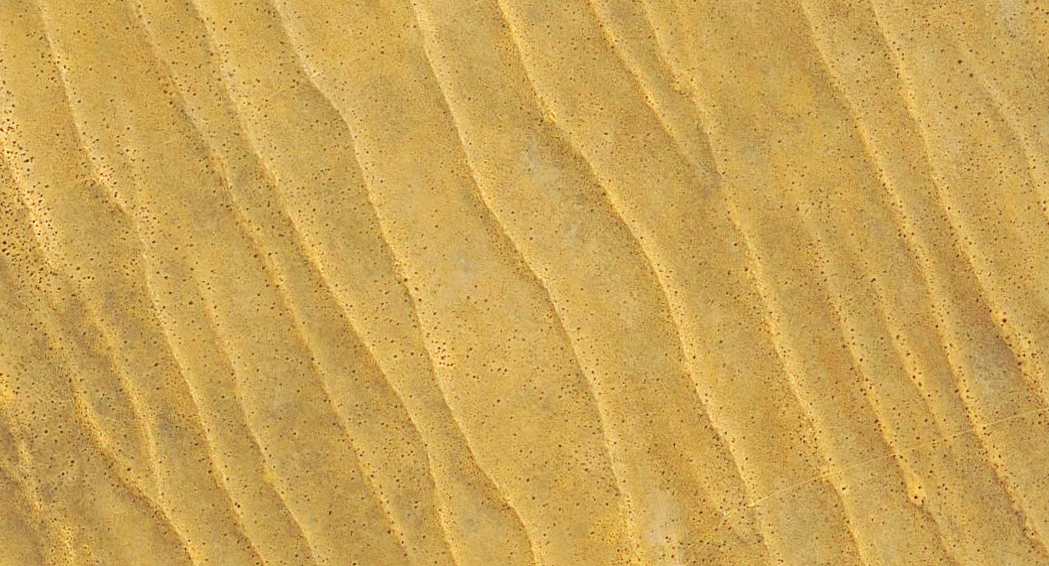
\includegraphics[width=\linewidth]{figures/kalahari}
 		\caption{Kalahari: Linear dune system}
 		\label{fig:difference_between_dune_field_types_kalahari}
 	\end{subfigure}
 	\begin{subfigure}{0.48\textwidth}
 		\centering
 		%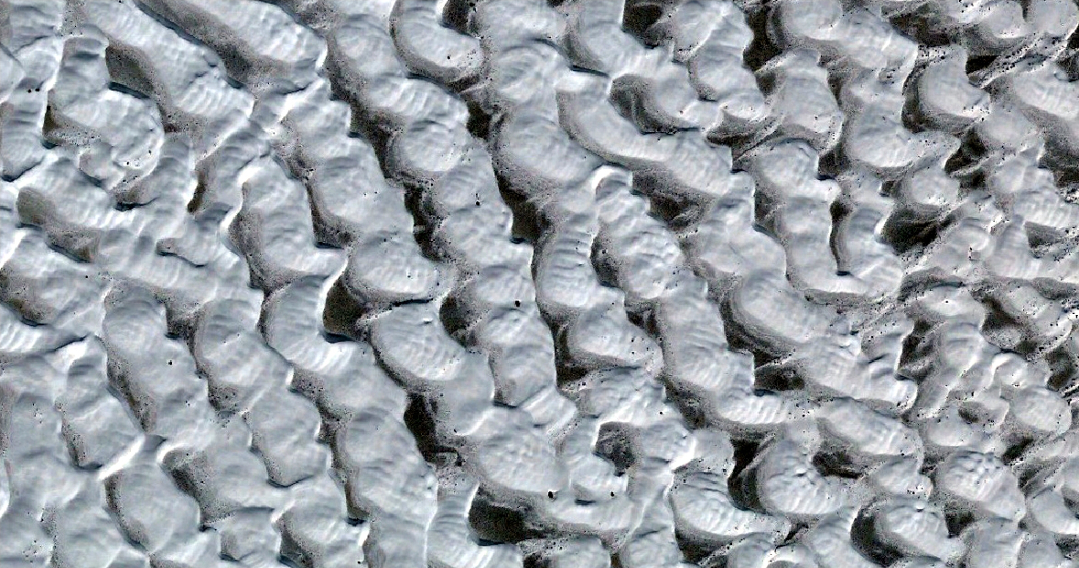
\includegraphics[width=\linewidth]{figures/whitesands}
 		\caption{White Sands: Complex dune system}
 		\label{fig:difference_between_dune_field_types_whitesands}
 	\end{subfigure}
 	
 	\caption{The variation in dune patterns such as \subref{fig:difference_between_dune_field_types_kalahari} linear, or \subref{fig:difference_between_dune_field_types_whitesands} complex, and the sun orientation and illumination effects on the resulting satellite images.}
 	\label{fig:difference_between_dune_field_types}
 \end{figure}
 
 Another important feature present dune crest-lines are the edges between the sunlit side and the shaded side. One assumption is that crest-lines produce relatively stronger edges than other areas of the image. This assumption was the principle guiding criteria in \cite{2015_automated_mapping_of_linear_dunefield}. However, the strength of the edge depends on many factors:
 
  \begin{enumerate}
	\item The sharpness of the actual dune ridge: dune which have sharper crest-lines will undoubtedly produce stronger, more defined edges on the satellite images.
	\item The sun's orientation and time of day: As the sun approaches the horizon, the sunlit and shaded sides of the dunes become more defined. Inversely, when the sun is higher in the sky, shadows become less pronounced. Also, as discussed previously, the orientation relative to the dune field itself affects the strength of the edges.
	\item Scale, noise and resolution of the image can all affect the strength of edges.
  \end{enumerate}

Understanding the issues with the gradients of the key problem of this research. As shown in Figure \ref{fig:patches}, the pixel values and gradient magnitudes (edge strength) can vary greatly in each region. One inclination is to select strong gradients in an image as candidates for crest-lines (as done in \cite{2015_automated_mapping_of_linear_dunefield}). However, the gradients of crest-lines are not always larger than the gradients of valleys or the shadows. 

In Figure \ref{fig:patches}, a plot of the intensity, gradient magnitudes, and gradient orientations along a cross section of a crest-line is shown. In the sample image patches \ref{fig:kalahari_patch}, \ref{fig:skeletoncoast_patch}, \ref{fig:wdc_patch}, the intensity values of the pixels along the direction shown are plotted in blue in Figures \ref{fig:kalahari_patch_plot}, \ref{fig:skeletoncoast_patch_plot}, \ref{fig:wdc_patch_plot}, the gradients magnitudes are shown in red, and the gradient orientations are shown in a dotted black line. 

\begin{figure}
	\centering
	\begin{subfigure}{0.15\textwidth}
		\centering
		%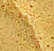
\includegraphics[width=\linewidth]{figures/kalahari_patch}
		\caption{}
		\label{fig:kalahari_patch}
	\end{subfigure}
	\begin{subfigure}{0.15\textwidth}
		\centering
		%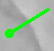
\includegraphics[width=\linewidth]{figures/kalahari_patch_arrow}
		\caption{}
		\label{fig:kalahari_patch_arrow}
	\end{subfigure}
	\begin{subfigure}{0.65\textwidth}
		\centering
		%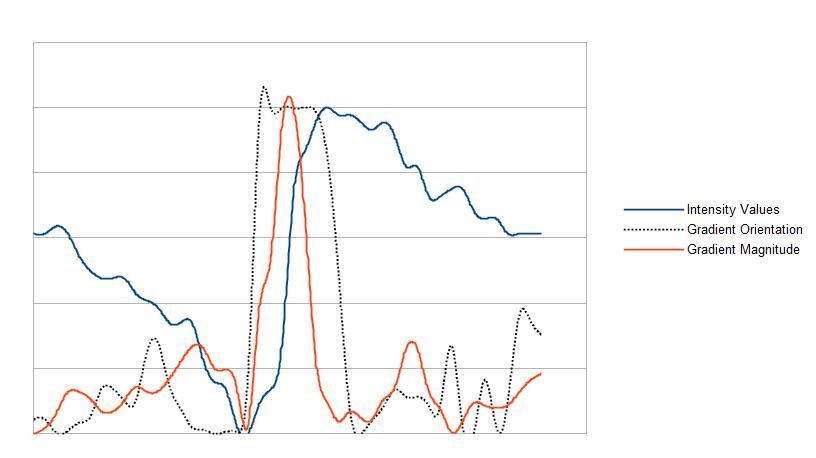
\includegraphics[width=\linewidth]{figures/kalahari_patch_plot}
		\caption{}
		\label{fig:kalahari_patch_plot}
	\end{subfigure}
	
	\begin{subfigure}{0.15\textwidth}
		\centering
		%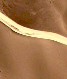
\includegraphics[width=\linewidth]{figures/skeletoncoast_patch}
		\caption{}
		\label{fig:skeletoncoast_patch}
	\end{subfigure}
	\begin{subfigure}{0.15\textwidth}
		\centering
		%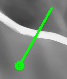
\includegraphics[width=\linewidth]{figures/skeletoncoast_patch_arrow}
		\caption{}
		\label{fig:skeletoncoast_patch_arrow}
	\end{subfigure}
	\begin{subfigure}{0.65\textwidth}
		\centering
		%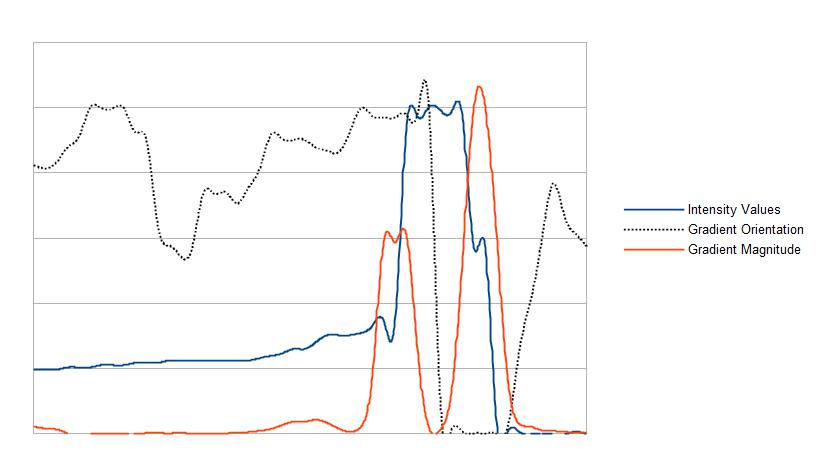
\includegraphics[width=\linewidth]{figures/skeletoncoast_patch_plot}
		\caption{}
		\label{fig:skeletoncoast_patch_plot}
	\end{subfigure}
	
	\begin{subfigure}{0.15\textwidth}
		\centering
		%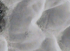
\includegraphics[width=\linewidth]{figures/wdc_patch}
		\caption{}
		\label{fig:wdc_patch}
	\end{subfigure}
	\begin{subfigure}{0.15\textwidth}
		\centering
		%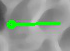
\includegraphics[width=\linewidth]{figures/wdc_patch_arrow}
		\caption{}
		\label{fig:wdc_patch_arrow}
	\end{subfigure}
	\begin{subfigure}{0.65\textwidth}
		\centering
		%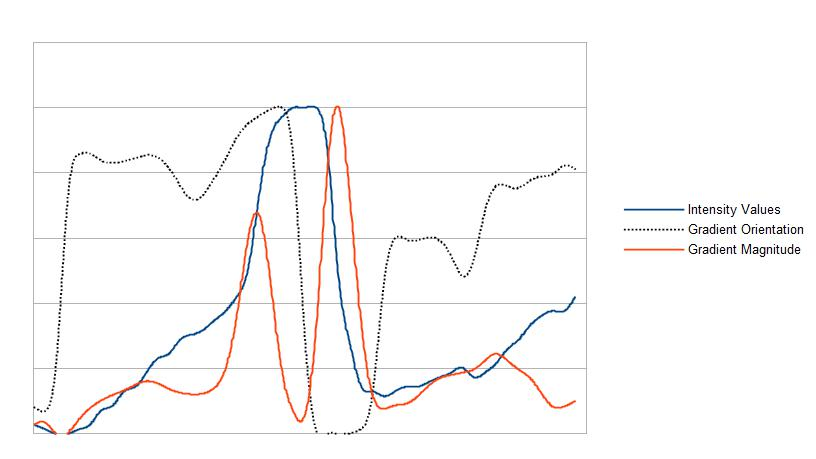
\includegraphics[width=\linewidth]{figures/wdc_patch_plot}
		\caption{}
		\label{fig:wdc_patch_plot}
	\end{subfigure}
	\caption{Illustration of the intensity, gradient magnitudes, and gradient orientations, plotted along a path crossing a dune crest-line: \subref{fig:kalahari_patch}, \subref{fig:skeletoncoast_patch},\subref{fig:wdc_patch} a sample image patch from Kalahari, Skeleton Coast, and White Sands regions, \subref{fig:kalahari_patch_arrow}, \subref{fig:skeletoncoast_patch_arrow}, \subref{fig:wdc_patch_arrow} the direction of the pixel samples plotted in \subref{fig:kalahari_patch_plot}, \subref{fig:skeletoncoast_patch_plot}, \subref{fig:wdc_patch_plot} containing the intensity, gradient magnitude and orientations values along the sampled direction. }
	\label{fig:patches}
\end{figure}

Typically, a peak in intensity values of the pixels is present, representing the sunlit side of a dune. Inevitably, this will produce two peaks in the gradient magnitude on both sides of the intensity peak. One of them represents the true crest-line of a dune, while the other can either be the shadow cast by the dune, or the bottom valley of the dune. The main difference between the two peaks, other than their gradient magnitude, is the fact they are almost always in opposite orientations. One peak is going from dark to bright, the other from bright to dark. If the sun's orientation relative to the dune field is known, then choosing the correct peak is trivial. When the orientation is unknown, choosing the correct peak becomes a challenging problem. 

In \cite{2015_automated_mapping_of_linear_dunefield}, the assumption was made that the weaker of the two edges can be filtered out, claiming that the larger peak is the crest-line, which is valid in the Kalahari image patch in Figure \ref{fig:kalahari_patch_plot}. However, the gradients produced by crest-lines may or may not be larger than their cast shadows, or the valleys. A clear example is shown in Figure \ref{fig:skeletoncoast_patch_plot}. In this scenario, the true crest-line is actually represented by the first gradient peak. The second peak is in fact produced by the shadow of a different dune.

Another interesting challenge is found in the images themselves. The correct crest-line cannot easily be determined by simple observation. A person presented with the image patch shown in \ref{fig:skeletoncoast_patch} would most likely not be able to determine with certainty which one of the edges represents the true crest-line. The obvious solution is to know the orientation of the sun relative to the dune field, but that may not always be possible.

All the challenges listed above need to be addressed in order to accurately and reliably detection dune crest-lines. In the next section, the overall process flow of the crest-line detection application is presented. Following sections will discuss the various approaches to solving the problems are presented as part of the research.

\subsection{Overall Process Flow}

In this research, many different approaches were attempted and compared to extract meaningful features from the images and compute the appropriate morphological properties of the dune fields. The overall process flow of detecting crest-lines can be represented as a five stage process:

 \begin{figure}[H]
 	\centering
 	%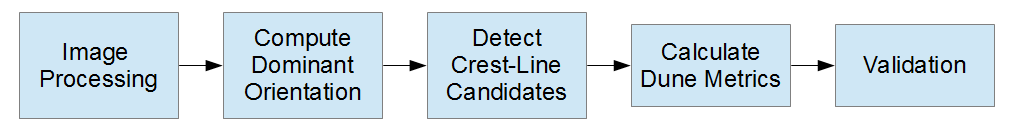
\includegraphics[width=\linewidth]{figures/flow1}
 	\caption{The overall process flow for general dune detection. The five steps include image processing, dominant orientation computation, crest-line candidate detection, calculations of dune metrics, validation of crest-line candidates.}
 	\label{fig:main_flow}
 \end{figure}

\subsubsection*{Image Processing}

The pre-processing stage is an important step to normalize and de-noise the input data. Image processing is typically a low level process which attempts to improve image quality, normalize illumination, or remove unnecessary noise from the image. This type of processing will in turn improve higher level feature extraction.

The first step is to insure that the images have roughly the same scale. To enforce scale normalization, the datasets scales were manually selected for appropriate crest-line detection application, and the image resolutions were resized to roughly 1000 pixel in width. The appropriate resolution is chosen based on a few factors:

\begin{itemize}
	\item Source resolution: The selected resolution is limited by the original image's resolution. No extra information can be gained from increasing the source image's resolution.
	\item Processing time: Higher resolution images require much more processing time overall which could be a limitation in a certain application.
	\item Scale selection: If the application's domain is found in a higher scale space, a higher resolution may not necessarily be required.
\end{itemize}

In this application, the goal is to detect the major crest-line, which is a higher scale domain, which means a higher resolution image is not a necessity. However, the parameter selection in these processes are dependent on the resolution and scale of the images. In future work, the dominant scale of the crest-lines could be determined automatically to improve the robustness of the algorithms.

The next step in the process is to convert the images to gray scale. The images in the terrestrial, and Ganges datasets (described in section \ref{subsec:terrestrial_dataset} and \ref{subsec:mars_dataset}) are color images by default. Although color processing of these images has not extensively been tested as part of this study, it is arguable whether using color information would improve the detection results. By converting the images to gray scale, an added benefit of normalizing the images across many region is implicitly enforced. Finally, the conversion process turns the three channel image into a single channel image which improves overall processing performance.

The final preprocessing step is to improve the image quality with low-pass filters. Many of the algorithms in this method rely on gradient information. Therefore, to extract the meaningful gradients, removing the highest frequencies (which in typically are responsible for noise), while preserving the lower scale or more desirable gradients. Two main popular filters are utilized. The median filter, introduced in \cite{huang_median_filtering_algorithm}, is applied first to remove grain and salt and pepper noise while preserving important edges. In some cases, median filtering also helps remove some smaller scale objects such as bushes, trees, rocks, and other features which are indistinguishable from satellite images. Following this, the standard Gaussian filter is applied which removes the remaining high frequency noisy signals from the image.

An important aspect to note is the size of the filter masks, which is heavily dependent on the resolution of the input image. We found that in most cases, for images around 1000 pixels in width, a \emph{sigma} value of approximately 1.5 and mask size of 7 by 7 was sufficient for this application. Once the image has been preprocessed, the gradients can be computed and saved for future use. Gradients can be computed by taking the first derivative of the image, using the popular Sobel operator.

An optional additional step is to apply histogram equalization to the image \cite{digital_image_processing_book}. Poorly illuminated or low contrast images greatly benefit from histogram equalization, because it stretches the contrast of the image in a consistent way. This in turns also helps in the extraction of edges, and improves determination of the dominant gradient orientation.

For the most part, the image processing step is common to most approaches proposed in this section. Some approaches require more or less pre-processing, but typically the processing is applied to each image before any detection is attempted.

\subsubsection*{Computing the Dominant Orientation} 
The dominant orientation is defined as the orientation of the gradients of crest-lines for the entire dune field. Computing the dominant orientation is an essential process in order to determine which gradients correspond to the actual crest-lines. This determination greatly improves the ability to filter out false positive candidates. In datasets where the sun's azimuth is known, the dominant orientation can be directly calculated using the sun's orientation. However, in cases where this information is not provided, the dominant orientation must be computed automatically. Sections \ref{subsec:dominant_orientation_k_means} and \ref{subsec:dominant_orientation_histogram_of_gradients} offer two main approaches to computing the dominant orientation.

\subsubsection*{Detecting Crest-Line Candidates}
The general crest-line candidate detection step extracts candidate segments which are most likely candidates for crest-lines. There are many potential methods to extract segments from the satellite images. The approaches explained in this section include appearance-based methods, which use the pixel values to extract crest-lines (\ref{subsection:appearance_based_approach} and \ref{subsec:watershed_transform_segmentation_approach}), gradient-based methods, which compute the derivatives of the images to extract the gradients (\ref{subsec:edge_based_detection} and \ref{subsec:gradient_orientation_based}), frequency domain methods (\ref{subsec:frequency_domain_approach}), and finally machine learning methods (\ref{subsec:machine_learning_approach} and \ref{subsec:mixed_ml_gradient_approach}). 

Each of these methods have slightly different processing flows but ultimately provide a way to extract candidate crest-lines. Once candidates have been extracted, some post-processing is often applied to reject some segments which do not fit the criteria of dune crest-lines. Rejected segments are typically filtered by length (too short), shape (too much curvature), weakness of gradients, or other factors. The remaining segments can also be smoothed in order to provide less noisy segments.

\subsubsection*{Dune Metrics Calculations}
Computing the dune metrics is the process of extracting the various geomorphological properties of the dune fields from the detected crest-lines. The two main metrics computed in this research are the orientation and inter-dune spacing. The reason these are the main important features is because they actually provide a large amount of information for researchers on the behavior of the dune fields. Additionally, they are fairly trivial to compute once dune crest-line segments have been extracted. Within the framework of this research, they can serve also as a proof of concept and validation of each crest-line detection method. 

In future work, other metrics, features, and properties could be computed, depending the specific research needs. The process of computing these metrics is discussed in detail in section \ref{subsec:dune-field-metrics}.

\subsubsection*{Validation}
The validation process evaluates the quality of each crest-line detector. In order to perform the validation, a dataset of ground truth is provided with each image. The main result metrics of the validation process are the precision and recall. Precision is the percentage of correctly identified crest-lines within the set of candidates. Recall is defined to be the percentage of correctly detected crest-lines from the ground truth. 

In addition, the validation process compares the results of the dune metrics calculations from the detected crest-lines and the ground truth. The same process of computing the dune metrics is also computed on the ground truth, and compared side-by-side with the detected crest-lines. The process is described in detail in section \ref{subsec:evaluation}.

The next section presents the first approach which is an appearance-based method.



\subsection{Appearance-Based Approach} \label{subsection:appearance_based_approach}
The appearance-based approach uses the pixel intensity values in the image to extract object regions. The process flow for this approach is shown in Figure \ref{fig:flow_appearance_based}. The goal of this approach is to extract the contours of bright regions in the images which are assumed to be the sunlit side of the dunes. The contours are then smoothed and filtered using the gradient magnitudes.

 \begin{figure}[H]
 	\centering
 	%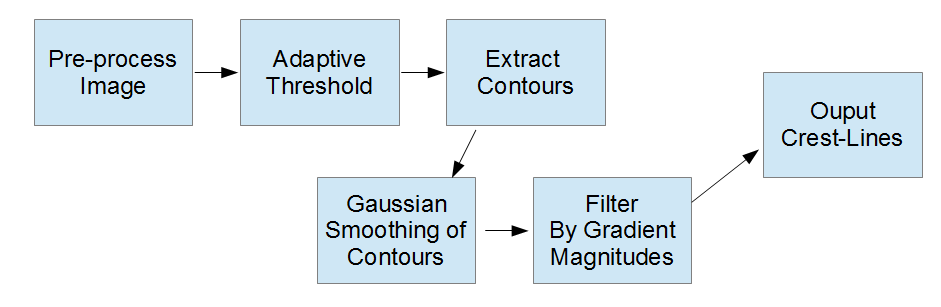
\includegraphics[width=\linewidth]{figures/flow_appearance_based}
 	\caption{The process flow of the appearance-based approach. The images are first preprocessed, then an adaptive threshold is applied to binarize the image. Contours are extracted from the resulting binary regions. The contour segments are smoothed and filtered by gradient magnitude, resulting in the detected crest-lines.}
 	\label{fig:flow_appearance_based}
 \end{figure}

As stated previously, dunes typically have a shaded and a sunlit side, and depending on the conditions and image quality, the actual edge or dune crest line may not be clearly defined. Image processing typically improves the quality and allow the extraction of the dune crest lines. The preprocessing step uses a simple low-pass filter to remove noise and median filter to remove additional noise and insignificant features.

Under the assumption that the sunlit side of the dunes are the relatively brightest regions in the image, a thresholding method can be applied to extract the light side of a dune. The process of thresholding (\cite{digital_image_processing_book}) is a common practice in image processing and computer vision. The process transforms the image into a binary (black and white) image for which regions can be extracted. The simplest thresholding method is to choose a fixed threshold value, and all pixels with intensity values greater than the threshold are set to 1 (white), and all others are set to 0 (black).

Using a fixed threshold may not be sufficient to extract the dunes since the illumination across an image is usually not uniform, and there may be poor contrast in intensity values. An adaptive threshold can be a useful tool to threshold an image with non-uniform illumination (\cite{1990_comparative_performance_study_thresholding,1979_threshold_selection_method_gray_level_histogram,2004_survey_over_image_thresholding_techniques}) An example of this type of thresholding is shown in Figure \ref{fig:adaptive_threshold}. 

\begin{figure}
	\centering
	\begin{subfigure}{0.48\textwidth}
		\centering
		%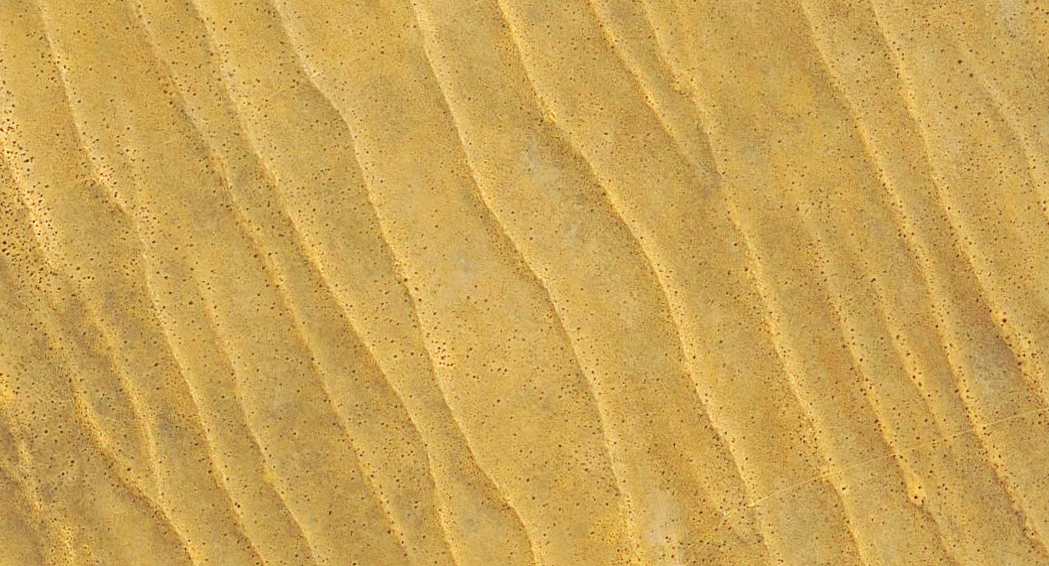
\includegraphics[width=\linewidth]{figures/kalahari}
		\caption{Kalahari Image}
		\label{fig:kalahari_adaptive_threshold_input}
	\end{subfigure}
	\begin{subfigure}{0.48\textwidth}
		\centering
		%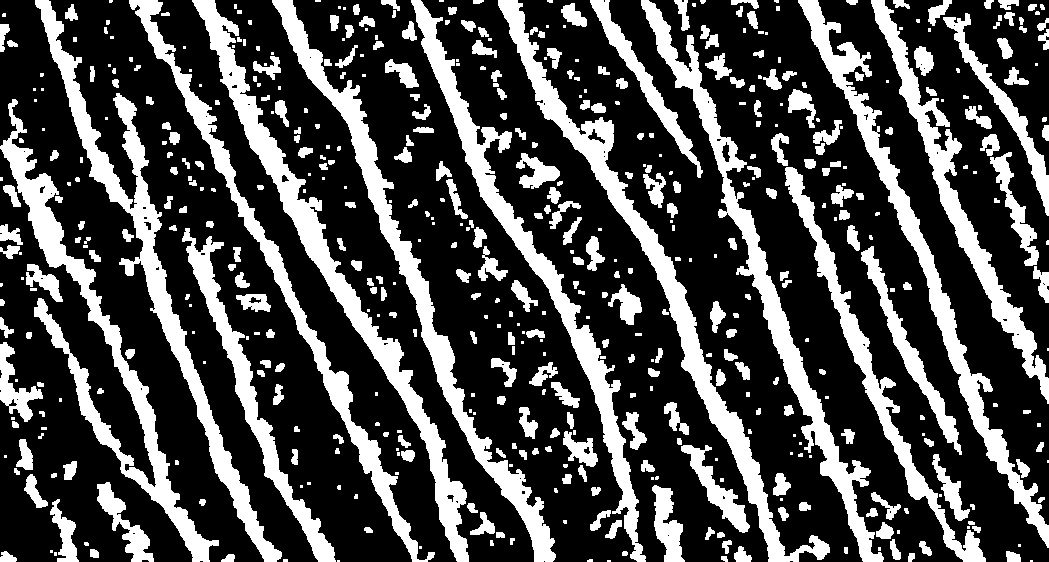
\includegraphics[width=\linewidth]{figures/kalahari_adaptive_threshold}
		\caption{Adaptive Threshold Binary Image}
		\label{fig:kalahari_adaptive_threshold}
	\end{subfigure}
	\caption{Adaptive Threshold applied to the Kalahari dune field satellite image. In \subref{fig:kalahari_adaptive_threshold_input} the Kalahari input image, \subref{fig:kalahari_adaptive_threshold} the adaptive threshold process applied to produce the binary image. }
	\label{fig:adaptive_threshold}
\end{figure}

Once the image has been preprocessed, the bright regions are extracted from the dune field image using an adaptive thresholding process, resulting in a binary image. As shown in Figure \ref{fig:adaptive_threshold}, the bright regions shown consist of the sun illuminated side of the dunes along with some noise. 

A region is defined as a contiguous group of pixels. From the regions, contours can be extracted, using a contour extraction algorithm described in \cite{opencv_library}. Each contour can then be filtered by size of the region. Smaller regions are considered as noise, and can be rejected from the dune candidates. The remaining region contours are used as potential candidates for dune crest lines.

The contours extracted should contain both the crest-lines themselves, and the base or valley of each dune, and they should be on opposite sides of the contours. Because the adaptive thresholding process tends to be noisy, the resulting contours will also be noisy. The contours are therefore smoothed using a Gaussian kernel defined as:

\begin{equation}
G\left(i\right)=\frac{1}{\sqrt{2\pi}\sigma}e^{\frac{-i^{2}}{2\sigma^{2}}}
\end{equation}

The Gaussian kernel is convolved on the contour, which a collection of two dimensional points $(x,y)$. The result of this convolution is a smoother contour which can be more reliably used as a dune crest line candidate. In order to filter out crest-line segments from non-crest-lines segments in the contours, we use the gradient magnitudes as a guide.

Typically, the assumption of this approach is that the dune crest lines are located on an area in the image where the derivatives are larger, or consistent along the edge of the dune. For each contour, the average magnitude $\mu$ of the derivative $\delta(i)$ of the image in the \emph{x} and \emph{y} directions is computed. Then, for each point within a contour compares its derivative with K neighbor's gradient magnitudes. Dune crest line candidate points will tend to have neighbors with similarly and consistently high gradients. To determine if a point $P(i)$ on a contour belongs on the dune crest line, we use the following criteria

\begin{equation}
P\left(i\right)=\begin{cases}
	1 & \phi(i)\geq r\\
	0 & otherwise
\end{cases}
\end{equation}

where

\begin{equation}
\phi(i)=\frac{\sum_{k=0}^{K}\begin{cases}
		1 & \delta\left(k\right)\geq\mu\\
		0 & \delta\left(k\right)<\mu
	\end{cases}}{K}
\end{equation}

and $0 < r \leq1$, which is the ratio of how many strong consistent edges to neighbors around a point i on the contour. Typically, \emph{r} would be larger than 0.5, which means most of the neighbors of a point most have strong edges for a point to be considered a dune crest line candidate. The parameter \emph{r} can be fine tune to allow more or less points to fit the criteria. This method will group common contour points based on gradient magnitude.

Once the dune crest line candidates on the contour have been extracted, the contour can be split into contiguous crest line segments. Some further processing can be applied to the segments, such as filtering out smaller or less significant segments (potential false positives). Overall, the approach does provide some valuable information, even though the results shown in Table \ref{tab:appearance_approach_results} of section \ref{subsec:results-and-discussion} are quite poor. The main problem with the approach is that there is too much variability in the input images causing the method to work well on some images, and quite poorly on others. The amount of parameters to tune for each specific dune region makes this method not a desirable approach for automated dune detection.

The next section presents an edge-based approach which relies on the gradients in the image to extract candidate crest-lines.



\subsection{Edge-based Approach} \label{subsec:edge_based_detection}

Unlike the appearance-based method previously presented, the edge-based methods used gradient information exclusively to detect crest-lines. The approach relies strongly on the assumption that crest-lines typically have relatively large gradients. The overall process flow is shown in Figure \ref{fig:flow_gradient_based}, which uses Canny edges and dominant orientation computation to determine which gradients belong to crest-lines. 

 \begin{figure}[H]
 	\centering
 	%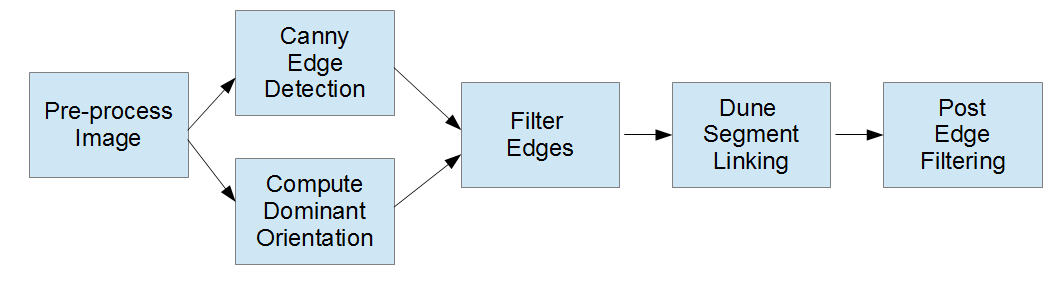
\includegraphics[width=\linewidth]{figures/flow_gradient_based}
 	\caption{The process flow of the gradient-based approach. The images are first preprocessed, then the Canny edge detection algorithm is applied to the image. The dominant orientation computation (\ref{subsec:dominant_orientation}), which enables many of the detected Canny edges to be filtered out based on orientation. The remaining edges are linked and post filtered based on length and shape.}
 	\label{fig:flow_gradient_based}
 \end{figure}

As stated previously, there are a few challenges specifically associated with extracting edges from the dune satellite images:

\begin{enumerate}
	\item Images tend to be noisy and highly textured, which results in many edges of varying orientations and magnitudes.
	\item Many of the stronger edges may not necessarily be the crest-lines themselves. Generally, dunes cast relatively large shadows which can themselves produce strong edges.
	\item Determining the appropriate values for the parameters of the edge detector can be difficult and greatly affect detection rates.
\end{enumerate}

To address the concerns stated above, the popular Canny edge detector (\cite{1986_canny_edge_detection}) is used along side some of the techniques inspired from \cite{Improved_Canny_Edge_Detection} and \cite{Runway_detection_tracking_unmanned}. First, in order to reduce the amount of noise in the images, both median and Gaussian filtering are applied to the image. The median filter removes small speckles (which for dune images may be small bushes or other contrasting features found in the images) while preserving major edge gradients. The Gaussian filter will then smooth out the gradient magnitudes and even out the image.

Once the image has been preprocessed, the Canny edge detector is used to recover the potential crest-line candidates. To overcome the parameter selection of the high and low threshold, the mean gradient $\mu$ and standard deviation $\sigma$ are computed over the entire image. The high and low thresholds are determined as follows:

\begin{equation}
T_{high}=\mu+q\centerdot\sigma
\end{equation}

\begin{equation}
T_{low}=\frac{T_{high}}{2}
\end{equation}

where \emph{q} is a factor which can be determined based on the problem set. This makes the threshold parameter less sensitive to fixed value threshold problems. The result of the Canny edge detector after filtering are displayed in Figure \ref{fig:canny_edges}. Clearly, the result of the Canny edge detector by itself is insufficient as many of the edges found are false positives. The next step in the process is to filter out the edge segments which do not belong to the dominant crest-lines.

 \begin{figure}
 	\centering
 	%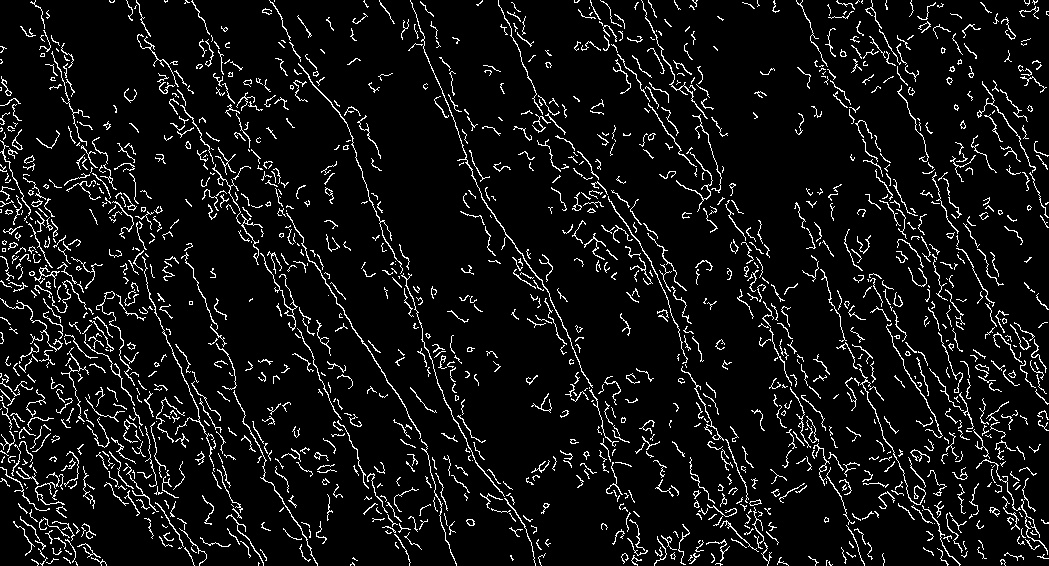
\includegraphics[width=0.90\textwidth]{figures/canny_edges}
 	\caption{Canny edge detector after median and Gaussian filtering of the Kalahari dune image.}
 	\label{fig:canny_edges}
 \end{figure}
 
 Many of the edges provided in the edge detection step are noise, shadows, and non crest-line textures. However, the crest-lines all have one distinctive feature in common: all of their gradient have relatively similar orientations. Similarly, because of the sun's orientation relative to the dune field, edges generated from the shadows of the dunes will also have similar orientations within themselves. Given these properties, there should be a clear delineation between crest-line edges, and non-crest-line edges. The next task then clearly becomes determining the orientation of the gradients which belong to crest-lines. This is accomplished by computing the dominant orientation of the image.
 
 \subsubsection*{Dominant Orientation Determination} \label{subsec:dominant_orientation}
 
 Computing the dominant orientation of the dune field is an important step in the process. The dominant orientation is the overall gradient direction of the crest-lines to be detected. This process can help determine the average orientation of the dune field as well. 
 
 An important point to make is that this process could be optional if the dominant orientation is known \emph{a priori}. Working with a dataset where the values are known improves the overall results of detection and enables skipping of this step. In cases where this information is unknown, or unavailable, automated dominant orientation determination is a potential solution.
 
 Typically, there exists a gradient peak at the crest-line peak of the dunes (although this may not always be the case for less pronounced dunes). The direction of the gradient should agree with the overall dominant orientation of the dune field. Computing the dominant orientation of the field can be challenging in many cases because dunes typically have two major orientations, which are opposite directions. This phenomenon is clearly illustrated in Figure \ref{fig:computing_dominant_orientation}. The true crest-line peak, where the sunny side meets the shaded side is one gradient (Figure \ref{fig:true_dominant_orientation_image}). At the foot of the dune, where the shaded returns to light, a second gradient will be present, whom has an opposite direction (Figure \ref{fig:false_dominant_orientation_image}).
 
 Two main methods have been implemented to determine the dominant orientation of the dune field.
 
 \subsubsection{Dominant Orientation From K-Means Clustering}\label{subsec:dominant_orientation_k_means}
 
 Resolving the dominant orientation can be achieved by grouping similar edges together by clustering the gradients.  The input data for clustering is the gradient vectors themselves. The gradient vectors are simply the first derivatives in the \emph{x} and \emph{y} directions: $\langle \delta_{x_{i}}, \delta_{y_{i}} \rangle$. Derivatives are typically computed by convolution of filters such as the Sobel operator (\cite{2014_history_sobel_operator}).
 
 There have been many approaches to clustering, but one of the simplest and most common is the K-Means algorithm (\cite{1965_Cluster_analysis_multivariate_data,1982_least_square_quantization_pcm,1967_method_classification_analysis_multivariate_observations}). The primary benefit of using a clustering algorithm is that it is unsupervised, therefore the dominant orientation can be inferred from the gradient vectors themselves.
 
 Typically, the main parameter that is required for K-Means is the value K, which is simply the number of clusters. In this problem set, the goal is to separate the crest-line group from all other non-crest-line edges. Therefore, clustering is computed using two clusters, by setting $K=2$. There may be some value in trying different number of clusters, but this was not investigated as part of this research. Some of the benefits include better separability of gradients.
 
 In order to get normalized results for the clustering algorithm, the gradients themselves are normalized. To normalize the gradients, the average gradient magnitude of the detected edges is computed as:
 
 \begin{equation}
  \bar{\delta_{\mu}}=\frac{\sum_{i=0}^{P}\sqrt{\delta_{x_{i}}^{2}+\delta_{y_{i}}^{2}}}{P}
 \end{equation}

 where P is the total number of detected edges from the Canny edge detector, $\delta_{x_{i}}$ and $\delta_{y_{i}}$ are the \emph{x} and \emph{y} gradient component of the \emph{i\textsuperscript{th}} point. Each gradient is then normalized by dividing by the average magnitude $\bar{\delta_{\mu}}$. This process is commonly called \emph{L2 normalization}.  

 \begin{equation}
 \dot{\delta}\left(x_{i},y_{i}\right)=\left(\frac{\delta_{x_{i}}}{\bar{\delta_{\mu}}},\frac{\delta_{y_{i}}}{\bar{\delta_{\mu}}}\right)
 \end{equation}

 The set of normalized gradient vectors are then clustered using the K-Means algorithm with $K=2$. In Figure \ref{fig:kmeans_results}, the results of the clustering method are shown. The blue points are gradient vectors which potentially belong to the dune crest-line. Studying the points, we notice that there is a skew towards the stronger edges in the blue cluster, which we will call the dominant cluster. This is determined by computing the centroids of each cluster. The cluster with the larger overall gradient magnitude is therefore assumed to be the dominant orientation and the set which contains the crest-line points.
 
 \begin{figure}
 	\centering
 	%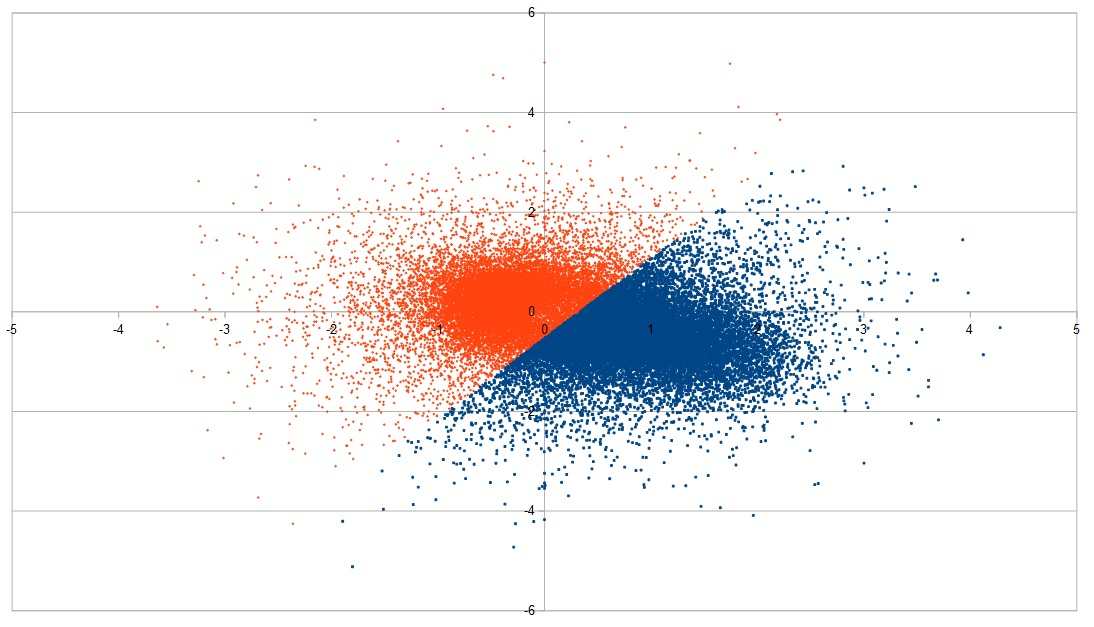
\includegraphics[width=0.90\textwidth]{figures/kmeans_results}
 	\caption{Results of K-Means clustering algorithm with $K=2$ on the edge gradients detected using Canny, from Kalahari. The blue cluster represents the dune crest-line gradient vectors, and the red points represents all other non-crest-line edges. The cluster centers of blue is $(0.8958, -0.5496)$, and the cluster center of the red is $(-0.4111, 0.2705)$. The cluster centers are used to determine the dominant orientation.}
 	\label{fig:kmeans_results}
 \end{figure}
 
 Once the clusters have been determined, all edges that agree (below to the dominant orientation cluster) are then assumed to be crest-line candidates. All other edges are filtered out. A sample of the filtering method is shown in Figure \ref{fig:kmeans_edge_results}.
 
  \begin{figure}
  	\centering
  	%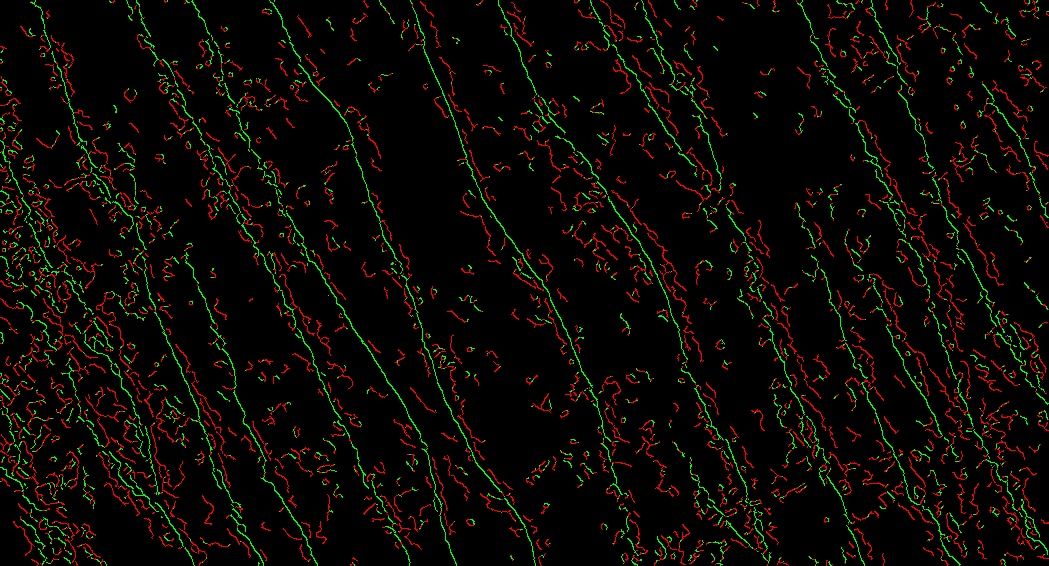
\includegraphics[width=0.90\textwidth]{figures/kmeans_cluster_results}
  	\caption{Results of filtering out edges which are not part of the dominant orientation (in red), while preserving edges which agree (in green) with the dominant orientation computed by the K-Means clustering method.}
  	\label{fig:kmeans_edge_results}
  \end{figure}
  
  Once the weak edges have been filtered out, the remaining edges are used as crest-line candidates. The K-Means cluster removes a majority of false positives, but does preserve some small edge segments which are most likely noise. By using a connected components technique, these smaller less significant edge segments can be removed, keeping only longer contiguous segments.
  
  \subsubsection{Dominant Orientation From Histogram of Gradients} \label{subsec:dominant_orientation_histogram_of_gradients}
  
An alternative to the clustering method is to compute a histogram of the gradients based on orientation. Histograms of gradient directions can be used to determine the true orientation. Histograms have been used for many processes and applications including \cite{lowe_sift_paper, dalal_histogram_oriented_gradients_human_detection, hu_gradient_field_descriptor}. Quantizing the space allows us to split edges according to their orientation, where each bin in the histogram represents an edge orientation. Each bin then covers an angle of $\frac{2\pi}{N}$radians, where \emph{N} is the number of bins. Each bin of the histogram is weighed by the magnitude of edges. Once the histogram is constructed, peaks in the magnitude will help determine the dominant orientation ($\varPhi$) of the dune crest-lines. The approach poses three main problems:
  
  \begin{enumerate}
  	\item Determining \emph{N}: In practice, a larger value for \emph{N} has shown to provide finer grain resolution which improves dominant orientation determination. In Figure \ref{fig:computing_dominant_orientation}, a value of $N=18$ is used (resulting in bins of $20\degree$ width).
  	\item Multiple Peaks: Often, images may have multiple peaks in the histogram, but only one of the peaks should represent the true dominant orientation of the crest-lines. As noted in \cite{2015_automated_mapping_of_linear_dunefield}, the histograms typically have a strong bimodal distribution, which is very apparent in Figure \ref{fig:dominant_orientation_histogram}.
  	\item Global Solution: The computed dominant orientation is global to the image, which may not be optimal in cases of complex dune structures. A better solution would be to compute the dominant orientation in a local area of the image, to account for local shifts in orientation.
  \end{enumerate}
  
  One assumption made is that the bin with the largest value represents the orientation of the crest-line edges. Although this assumption holds for many cases, it is not always the case. The Skeleton Coast test image provides a good example of this case in Figure \ref{fig:computing_dominant_orientation}. In this particular case, the are two major peaks in the histogram, where the stronger is not the part of the crest-line edge group, and the weaker one is. Choosing the higher peak will cause invalid crest-lines to be chosen. In order to determine which peak best represents the crest-line edge group, some normalization can be applied. The normalization process begins by computing the mean vector of the gradients from the edge image as follows:
  
  \begin{equation}
  \hat{\mu}\left\langle \bar{x},\bar{y}\right\rangle =\left\langle \frac{\sum_{i=0}^{P}\delta_{x_{i}}}{P},\frac{\sum_{i=0}^{P}\delta_{y_{i}}}{P}\right\rangle 
  \end{equation}
  
  where \emph{P} is the total number of detected edges from the Canny edge detector, $\delta_{x_{i}}$ and $\delta_{y_{i}}$ are the \emph{x} and \emph{y} gradient component of the \emph{i}\textsuperscript{th} point. The mean orientation is computed from the mean vector as:
  
  \begin{equation}
\bar{\theta_{\mu}}=\arctan\left(\frac{\mu_{\bar{y}}}{\mu_{\bar{x}}}\right)
  \end{equation}
  
  The gradients are then normalized by simply subtracting the mean vector from each gradient:
  
  \begin{equation}
\dot{\delta}\left(x_{i},y_{i}\right)=\left(\delta_{x_{i}}-\mu_{\bar{x}},\delta_{y_{i}}-\mu_{\bar{y}}\right)
  \end{equation}
  
  The normalized orientation $\dot{\theta_{i}}$ can be computed:
  
  \begin{equation}
  \dot{\theta_{i}}=\arctan\left(\frac{\dot{\delta_{y_{i}}}}{\dot{\delta_{x_{i}}}}\right)
  \end{equation}

  \begin{figure}
  	\centering
  	\begin{subfigure}{0.48\textwidth}
  		\centering
  		%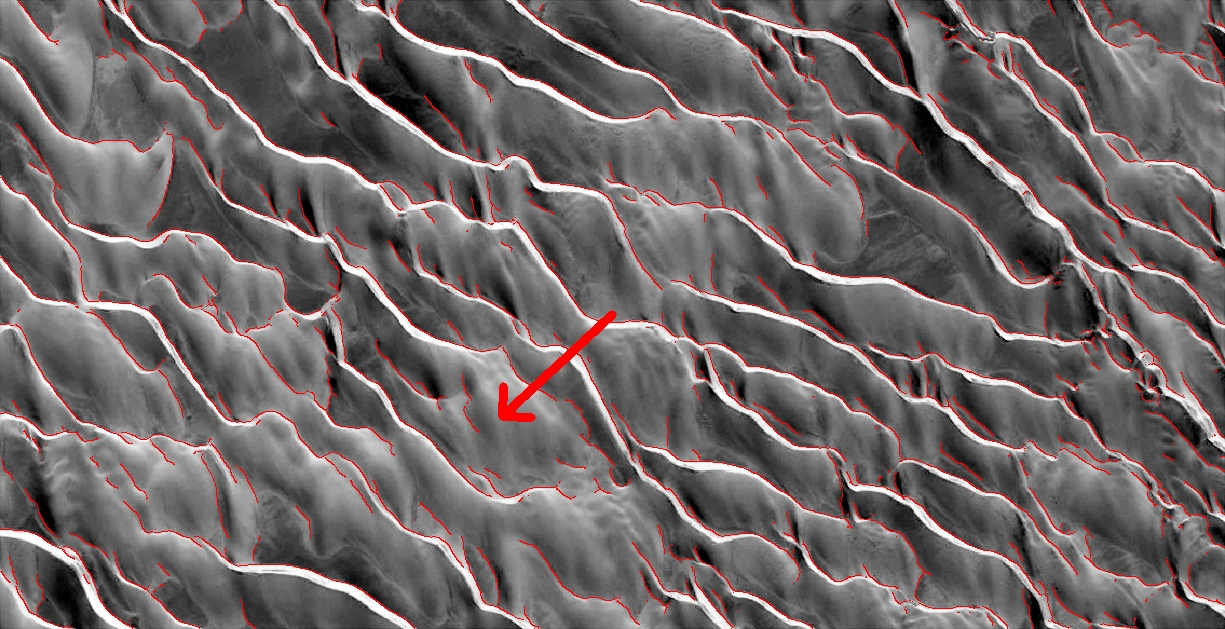
\includegraphics[width=\linewidth]{figures/dominant_orientation_false}
  		\caption{Non-Crest-line Edges}
  		\label{fig:false_dominant_orientation_image}
  	\end{subfigure}
  	\begin{subfigure}{0.48\textwidth}
  		\centering
  		%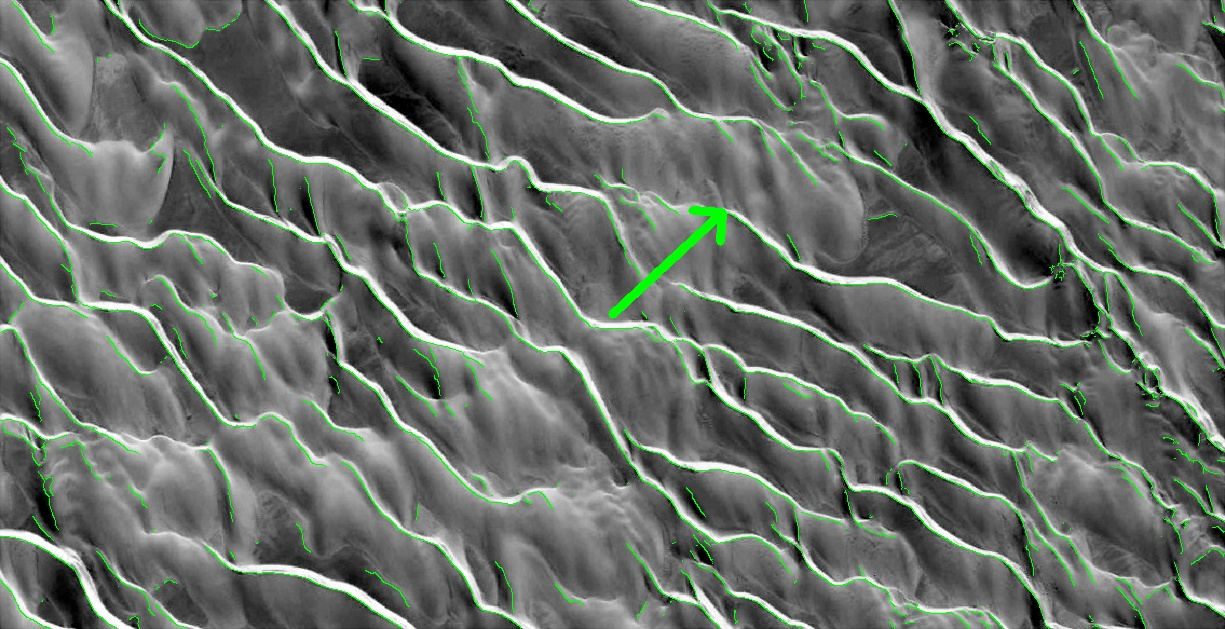
\includegraphics[width=\linewidth]{figures/dominant_orientation_true}
  		\caption{Crest-line Edges}
  		\label{fig:true_dominant_orientation_image}
  	\end{subfigure}
  	\begin{subfigure}{\textwidth}
  		\centering
  		%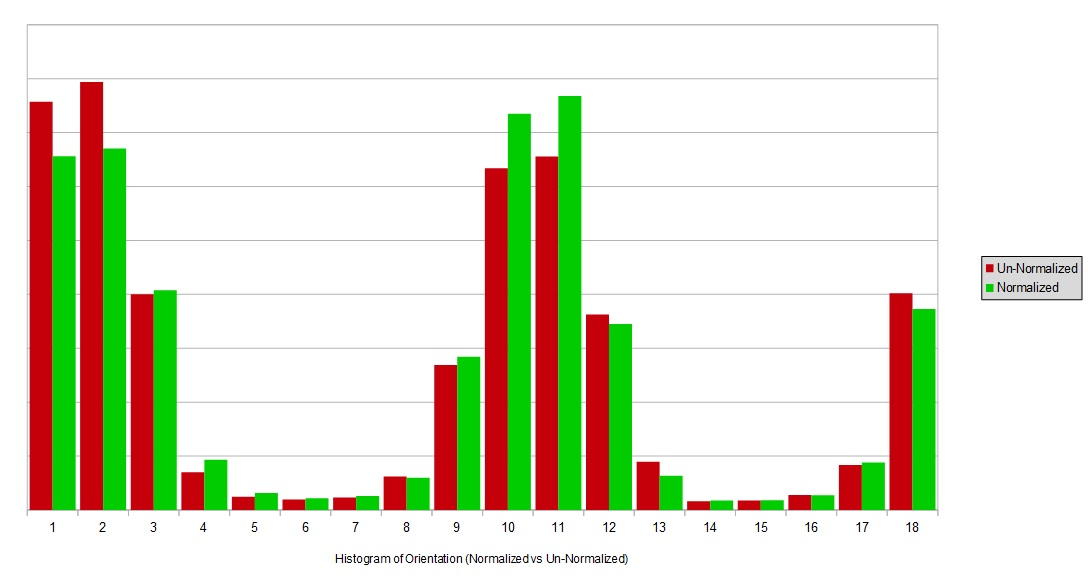
\includegraphics[width=0.8\linewidth]{figures/dominant_orientation_histogram}
  		\caption{Histogram of Gradient Orientations}
  		\label{fig:dominant_orientation_histogram}
  	\end{subfigure}
  	\caption{Results of unnormalized (red) and normalized (green) histograms of gradients orientations ($N=18$), where each represents a $20\degree$ slice. The histogram contains two major peaks, but the crest-line is the weaker of the two peaks. \subref{fig:false_dominant_orientation_image} Edges which belong to the dominant orientation which are invalid crest-lines. \subref{fig:true_dominant_orientation_image} With normalization, the true crest-lines now have the higher overall magnitude. \subref{fig:dominant_orientation_histogram} The 18 bin histogram of gradients with and without normalization.}
  	\label{fig:computing_dominant_orientation}
  \end{figure}
  
  To determine which bin the \emph{i}\textsuperscript{th} edge point belongs to, we simply calculate $\left\lceil \frac{\dot{\theta_{i}}\centerdot N}{2\pi}-0.5\right\rceil $,	and increment that bin by the magnitude of the normalized gradient	by $\sqrt{\dot{\delta}_{x_{i}}^{2}+\dot{\delta}_{y_{i}}^{2}}$. In essence, this normalization process removes the uneven skew of the gradients in the overall image. Removing this skew allows true crest-line edges to be fairly compared with other stronger edges. As shown in Figure \ref{fig:computing_dominant_orientation}, the normalization process softens the stronger dominant edge and enhances the true crest-line edges. This process enables true crest-lines to be accurately determined in images where the valleys of dunes are sharp and contain strong edges.
  
  Once the histogram is computed and normalized, the dominant orientation vector $\hat{\theta_{dom}}$ is determined by averaging the gradients belonging to the histogram bin with the highest value. With the dominant orientation knowledge acquired, candidate crest-line dunes can be detected.
  
  \subsubsection{Dune Segment Linking}
  
  With the dominant orientation computed, many false positives have been rejected. The next step of the process is to group segments which link together. Since each crest-line candidate segments is a collections of two dimensional points, an intuitive step is to fit a line to the candidate segments. The line fitting algorithm used is from the OpenCV library \cite{opencv_library}, which aims to minimize:
  
  \begin{equation}
  \sum_{i}\rho\left(r_{i}\right)
  \end{equation}
  
  where $r_{i}$ is the distance between a point an the line, and $\rho\left(r_{i}\right)$ is the function used. We use the simplest least square method, $\rho\left(r\right)=\frac{r^{2}}{2}$. The result of the line fitting produces a vector of four values $\left\langle x,y,v_{x},v_{y}\right\rangle$, where the $(x, y)$ components are the position of the line, and $(v_{x},v_{y})$ is the normalized vector which is collinear to the line, encoding the orientation of the line.
  
  Once all segments are fit with a line, we can filter the segments based on the orientations of the lines. To get a general view of the distribution of the orientation of the lines, a histogram of the line orientations can help determine dominant lines. The histogram can be constructed based on the orientation of the lines, weighed by segment length. As shown in figure \ref{fig:linehistogram}, the histogram appears to have a unimodal distribution. When choosing all lines which belong to the peak bin in the histogram, the resulting in the output image \ref{fig:filtered_edges_lines} The results show that many of the false positives have been filtered out.
  
  \begin{figure}
  	\centering
  	\begin{subfigure}{0.48\textwidth}
  		\centering
  		%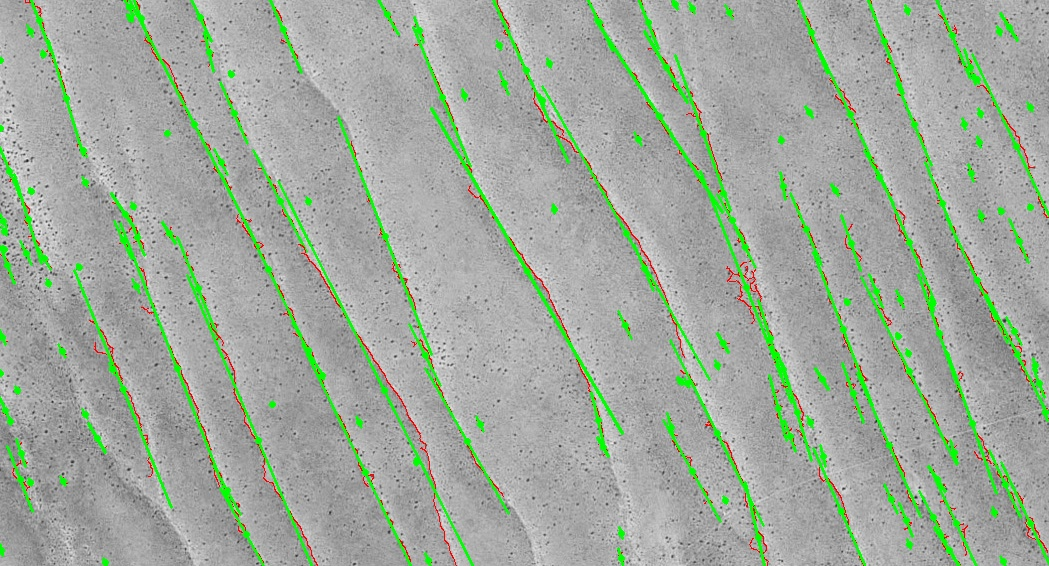
\includegraphics[width=\linewidth]{figures/filtered_edges_lines}
  		\caption{Line fitting to edge segments}
  		\label{fig:filtered_edges_lines}
  	\end{subfigure}
  	\begin{subfigure}{0.48\textwidth}
  		\centering
  		%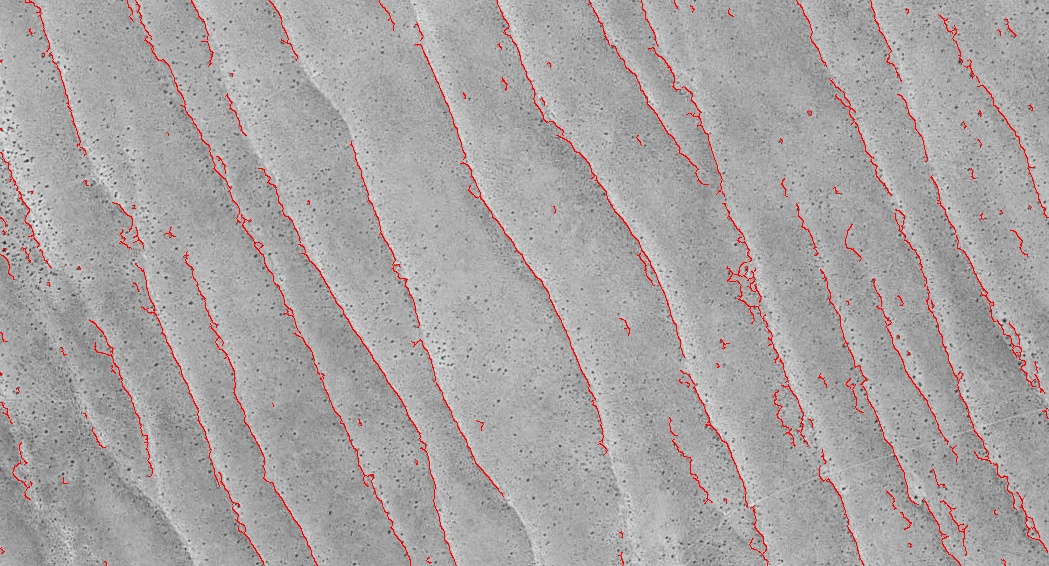
\includegraphics[width=\linewidth]{figures/filtered_edges}
  		\caption{Filtered edge segments}
  		\label{fig:filtered_edges}
  	\end{subfigure}
  	\begin{subfigure}{\textwidth}
  		\centering
  		%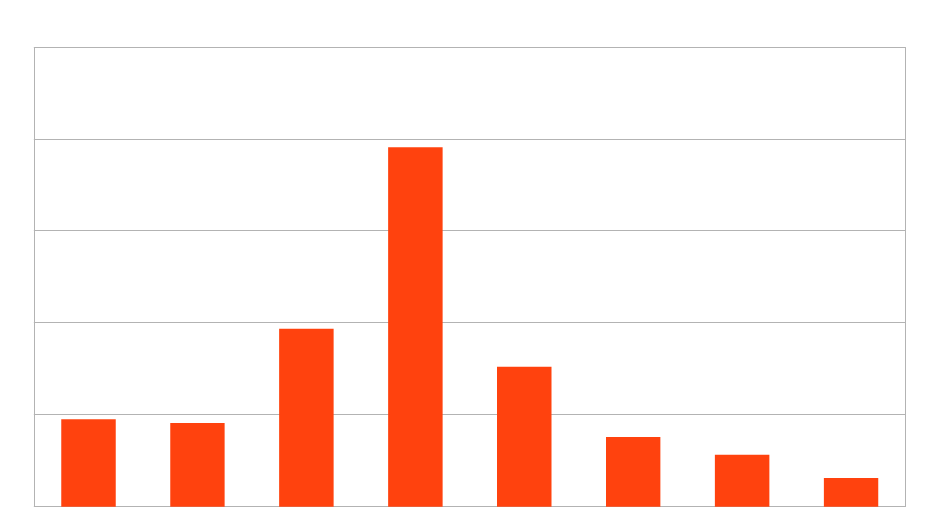
\includegraphics[width=0.50\linewidth]{figures/linehistogram1}
  		\caption{Histogram of line orientations}
  		\label{fig:linehistogram}
  	\end{subfigure}
  	\caption{Results of filtering based on the line orientation fitting, and choosing the peak in the histogram. In  \subref{fig:filtered_edges_lines} the fitted lines from the dune segments, \subref{fig:filtered_edges} segments which have orientation matching the peak in the histogram, \subref{fig:linehistogram}  the histogram of line orientations weighed by segment length. }
  	\label{fig:dune_segment_linking_line_fitting}
  \end{figure}
  
Since the shown distribution appears to be unimodal, a better approach may be to simply compute the mean and standard deviation of the line orientations. Choosing the appropriate sigma value to filter out the noise and false positives depends on the distribution. In some cases, such as images with crest-lines which are more curved, the variation orientations may be more significant. In order to avoid the filtering of true positives, a linking algorithm should be used to link segments which belong to the same crest-line.

The next section presents another appearance-based approach which utilizes the Watershed Transform to detect dune crest-lines.

\subsection{Watershed Transform Segmentation Approach} \label{subsec:watershed_transform_segmentation_approach}

Similarly to \ref{subsection:appearance_based_approach}, the goal of this approach is to segment out the brighter region of the image, which represents the sunny side of the dune, using the watershed transform. The overall process of this approach is shown in Figure \ref{fig:flow_watershed}.

 \begin{figure}[H]
 	\centering
 	%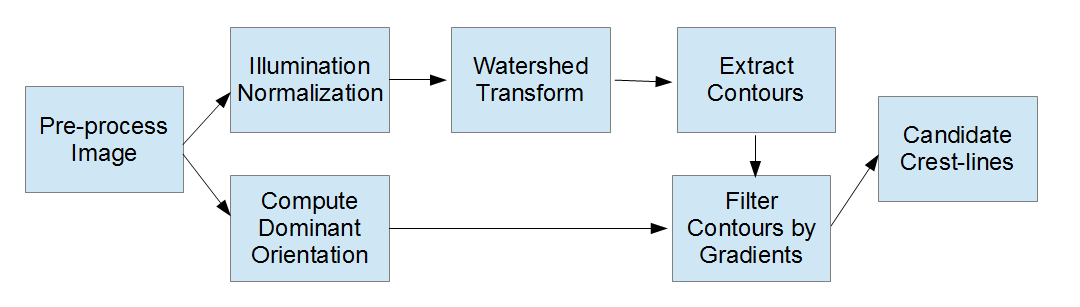
\includegraphics[width=\linewidth]{figures/flow_watershed}
 	\caption{The process flow of the Watershed Transform dune detection approach. The images are first preprocessed, then some illumination normalization is applied to the image in order to improve the results of the Watershed transform. Contours are then extracted from the resulting regions which are filtered using the gradients, based on the dominant orientation. }
 	\label{fig:flow_watershed}
 \end{figure}
 
  The watershed transform (\cite{2014_priority_flood,1979_workshop_image_processing,1994_watershed_continuous_function}) is a powerful segmentation tool, which in this approach is used to determine the boundary of the bright dune region. Typically, this approach can produce better results than a simple thresholding method. In order to extract reliable regions, image illumination normalization is applied, as shown in Figure \ref{fig:illumination_normalization}, to make the illumination more evenly distributed across an image. After applying some preprocessing to the image (again, median and Gaussian blurring to remove as much noise as possible), the illumination normalization presented is very basic, and better normalization schemes should be tried.

\begin{figure}
	\centering
	%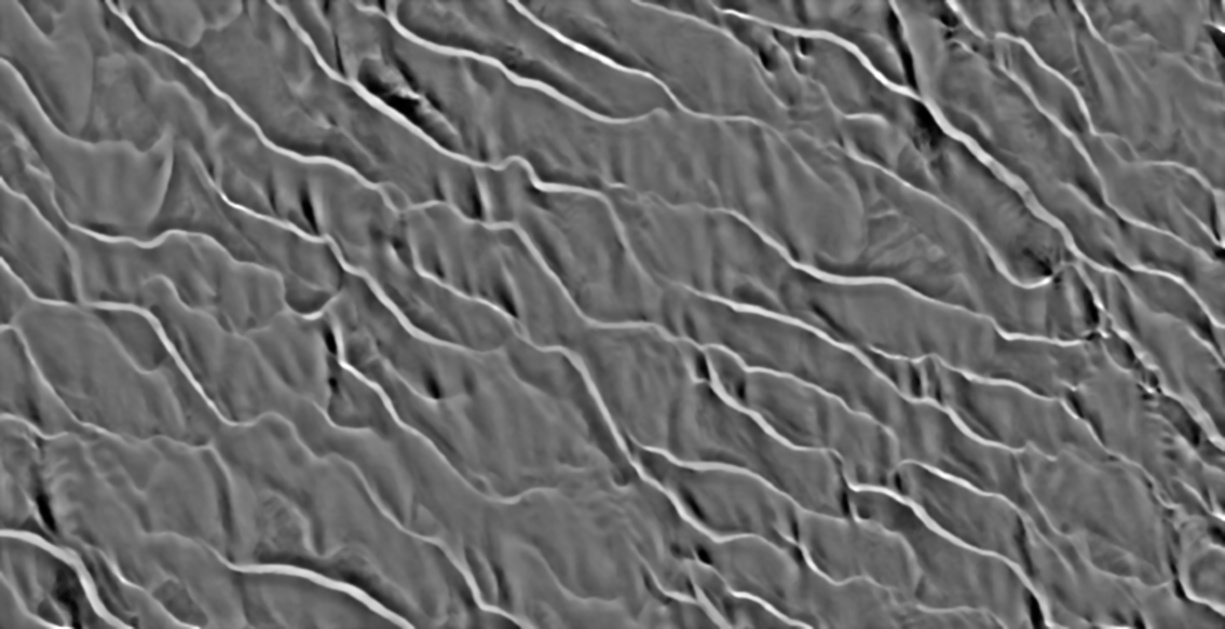
\includegraphics[width=0.90\textwidth]{figures/normalizedIllumination}
	\caption{Simple illumination normalization algorithm applied to the Skeleton Coast image.}
	\label{fig:illumination_normalization}
\end{figure}

The normalization process is done in a fairly simple and efficient way, using integral images. The integral image concept was originally proposed in \cite{Summed-area-tables-for-texture-mapping}, and was popularized for computer vision applications by \cite{Robust-real-time-Object-Detection}. The integral image representation allows rectangular features to be computed very efficiently. Each pixel $(x,y)$ of the integral image is the sum of the pixels above and to the left of it, as described in \cite{Robust-real-time-Object-Detection}:

\begin{equation}
ii\left(x,y\right)=\sum_{x'\leq x,y'\leq y}i\left(x',y'\right)
\end{equation}

To normalize using integral images, the mean $\mu_{i}$ of the image, which can be done efficiently once the integral images is computed, given an $N\times M$ image.

\begin{equation}
\mu_{i}=\frac{ii\left(M,N\right)}{M\cdot N}
\end{equation}

The goal of the illumination normalization is to bring pixel intensities value closer to the mean intensity of the image for a more even distribution of intensities. To accomplish this, we simply compute a ratio multiplier of the mean intensity $\mu_{i}$ over the square local area $(w\times w)$ mean intensity centered around a pixel $(x,y)$. The mean of a local area can be computed efficiently using the integral image theory:

\begin{equation}
\mu_{l}\left(x,y\right)=D-C-B+A
\end{equation}

\begin{equation}
A=ii\left(x-\frac{w}{2},y-\frac{w}{2}\right)
\end{equation}

\begin{equation}
B=ii\left(x+\frac{w}{2},y-\frac{w}{2}\right)
\end{equation}

\begin{equation}
C=ii\left(x-\frac{w}{2},y+\frac{w}{2}\right)
\end{equation}

\begin{equation}
D=ii\left(x+\frac{w}{2},y+\frac{w}{2}\right)
\end{equation}

Then, the ratio of image intensity to local mean intensity simply is $r_{\mu_{l}\left(x,y\right)}=\frac{\mu_{i}}{\mu_{l}\left(x,y\right)}$. The pixel intensity value at that location is then multiplied by this ratio to get the normalized value:

\begin{equation}
\tilde{i}\left(x,y\right)=r_{\mu_{l}\left(x,y\right)}\cdot i\left(x,y\right)
\end{equation}

With the image illumination normalized, the watershed transform can be used to segment out the brighter regions of the image which will be the dune sunny sides. The watershed implementation used is provided by the OpenCV library, and is a variant of the implementation proposed in \cite{Color-image-segmentation}. The watershed uses an initial seed rough image of the desired locations to segment out, which in this application is the brighter regions of the image. The desired regions to extract are the bright and shaded areas. The threshold values for these can be determined from the image's mean and standard deviation intensity values:

\begin{equation}
T_{high}=\mu_{i}+\rho_{high}\cdot\sigma_{i}
\end{equation}

\begin{equation}
T_{low}=\mu_{i}+\rho_{low}\cdot\sigma_{i}
\end{equation}

Where the $\rho_{high}$ and $\rho_{low}$ are scalar values determined empirically. All pixels above the high threshold are labeled as the desired region to segment (in white) as shown in Figure \ref{fig:watershed_sunlit_side}, and all pixels below the lower threshold are set to the non-desired region (in gray), shown in \ref{fig:watershed_shaded_side}. A morphological eroding operation is applied to better separate the regions for the watershed transform. Using the labeled image and normalized illumination image, the watershed algorithm is able to segment out the dune regions reliably, as shown in \ref{fig:watershed_segmentation}. 

 \begin{figure}
 	\centering
 	\begin{subfigure}{0.48\textwidth}
 		\centering
 		%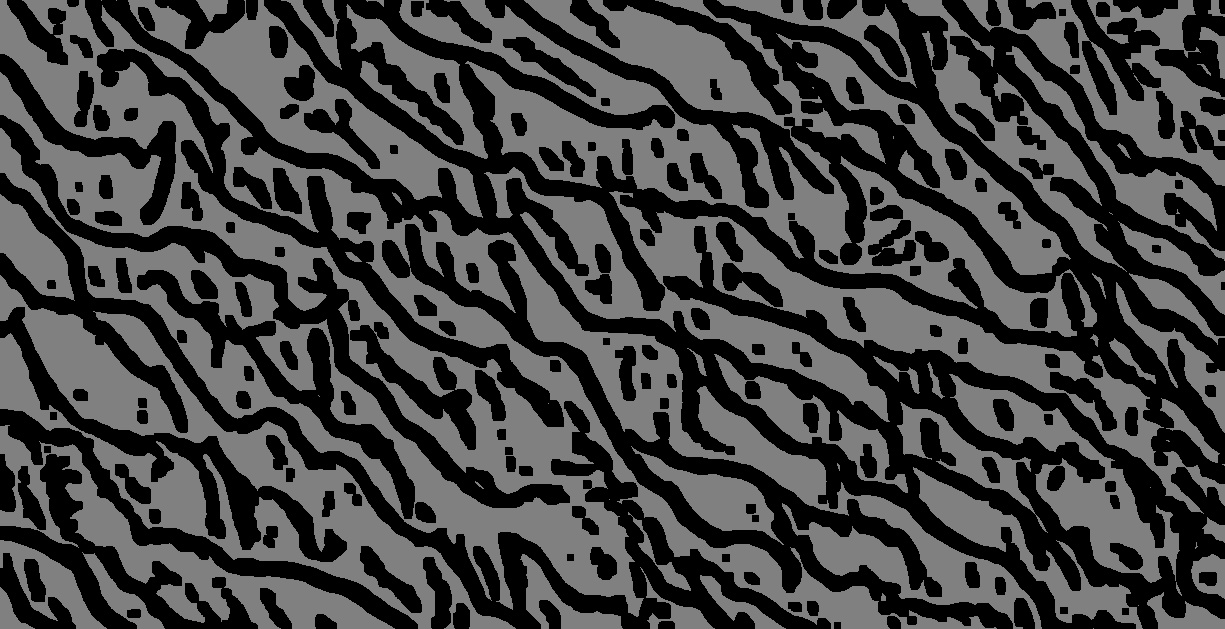
\includegraphics[width=\linewidth]{figures/watershed_shaded_side}
 		\caption{\emph{Shaded} region labels}
 		\label{fig:watershed_shaded_side}
 	\end{subfigure}
 	\begin{subfigure}{0.48\textwidth}
 		\centering
 		%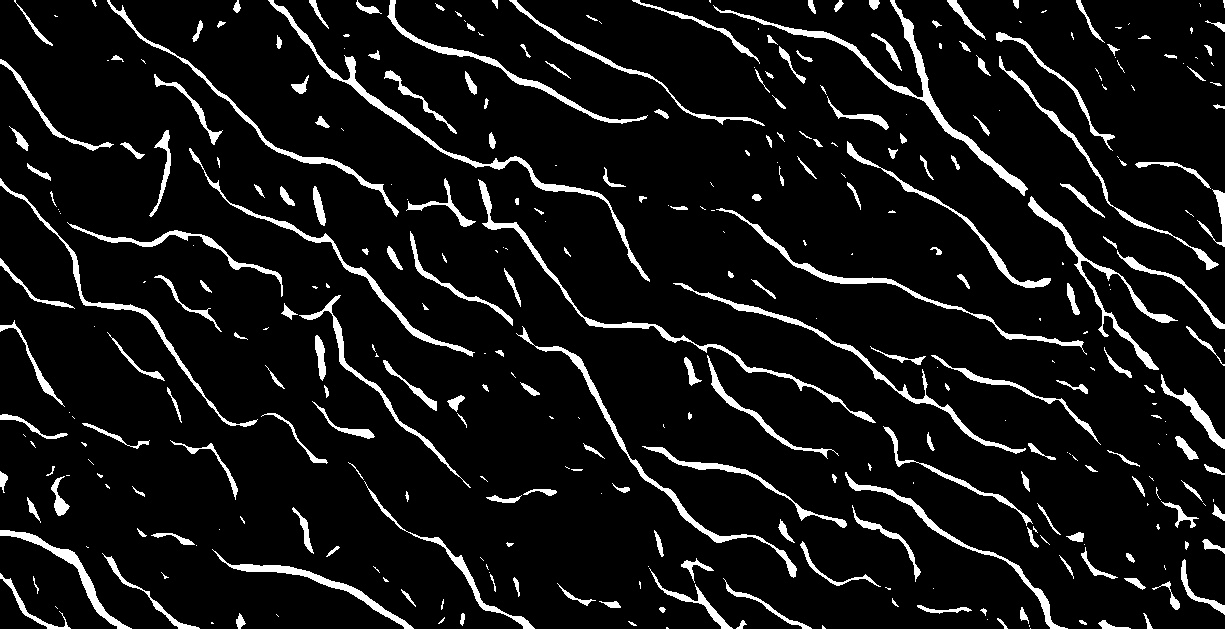
\includegraphics[width=\linewidth]{figures/watershed_sunlit_side}
 		\caption{\emph{Sunlit} region labels}
 		\label{fig:watershed_sunlit_side}
 	\end{subfigure}
 	\begin{subfigure}{0.48\textwidth}
 		\centering
 		%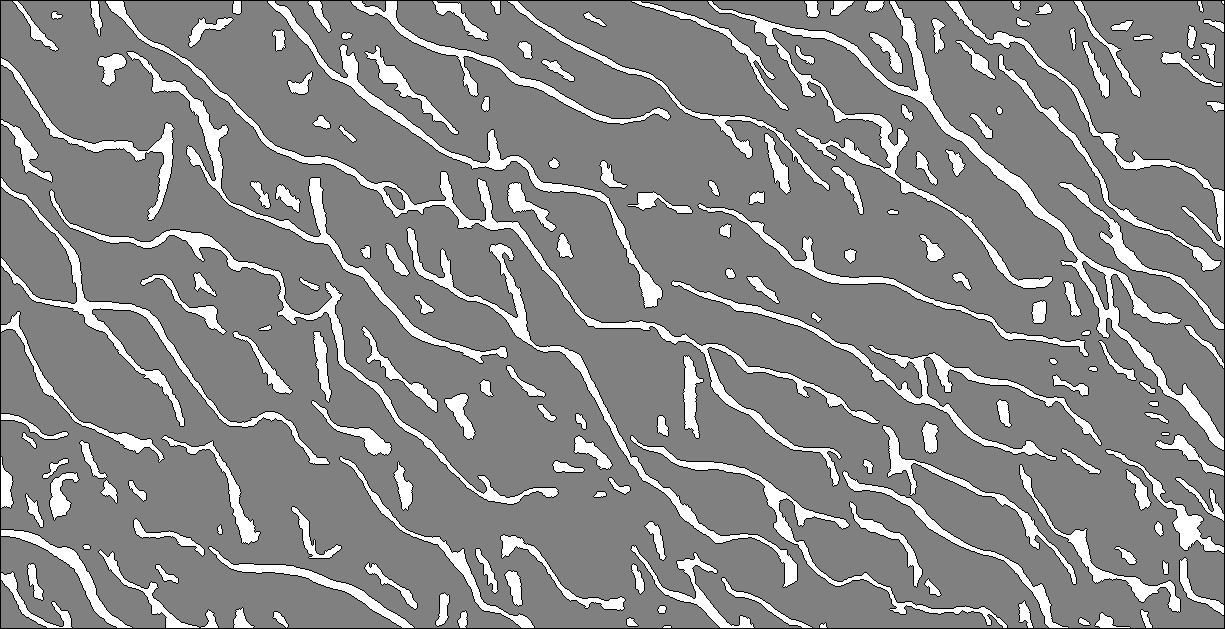
\includegraphics[width=\linewidth]{figures/watershed_segmentation}
 		\caption{Watershed Transform}
 		\label{fig:watershed_segmentation}
 	\end{subfigure}
 	\begin{subfigure}{0.48\textwidth}
 		\centering
 		%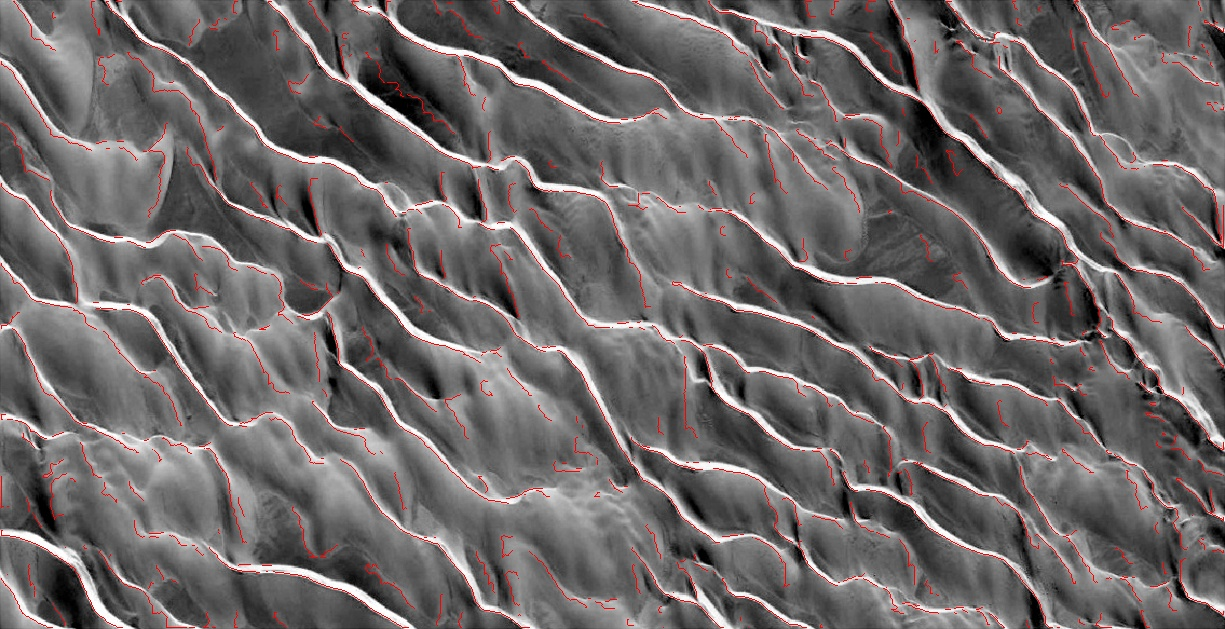
\includegraphics[width=\linewidth]{figures/watershed_dune_detection}
 		\caption{Results}
 		\label{fig:watershed_dune_detection}
 	\end{subfigure} 
 	\caption{Watershed Transform results example applied to the Skeleton Coast. In \subref{fig:watershed_shaded_side}, the pixels labeled as \emph{shaded}, \subref{fig:watershed_sunlit_side} the pixels labeled as \emph{sunlit}, \subref{fig:watershed_segmentation} the output of the Watershed Transform, and \subref{fig:watershed_dune_detection} crest-line detection results from the Watershed Transform. }
 	\label{fig:watershed_results}
 \end{figure}

After computing the watershed segmentation image, the regions extracted from it can be retrieved using contour detection. The contours retrieved are closed loops where one segment will be along the dune crest line and the other not. To determine which segments of the contour belong to the dune crest-line, we can use what was learned from section \ref{subsec:dominant_orientation_histogram_of_gradients}: Building a histogram of the image gradients, choosing the dominant orientation, and filtering out all contour points which do not agree with the dominant orientation. 

Results can be seen in Figure \ref{fig:watershed_results}. Although the results appear promising, the Watershed transform method has a few drawbacks:

\begin{itemize}
	\item An assumption that a dune contains a bright side. Not all images (especially the Simpson image), have crest-lines that have a bright edge.
	\item The edges of the contours appear to be slightly noisier than edge-based approaches.
	\item Localization of the segments is poor. Some segments do not lie on an actual edge, which may be reported as a false positive.
\end{itemize}

On the other hand, the watershed approach does appears to have some key benefits:

\begin{itemize}
	\item Better connectivity of dune crest-line segments. When edges become weak between two connecting segments, the edge based approaches produce gaps, where the watershed is able to fill the gaps.
	\item Watershed method could be further expanded to include color image processing.
\end{itemize}

The next section explores another approach which utilizes the frequency domain to extract crest-lines.


\subsection{Frequency Domain Approach} \label{subsec:frequency_domain_approach}

In this approach, we take advantage of the fact dune-field patterns seem to to have some periodic pattern, which could possibly be extracted from the frequency domain. Converting the images into the frequency domain using the Discrete Fourier Transform (DFT) (\cite{1988_fast_fourier_transform_applications,1969_finite_fourier_transform}) provides a method for applying some processing on individual frequencies of the image. The process flow for this approach is shown in Figure \ref{fig:flow_dft}.

 \begin{figure}[H]
 	\centering
 	%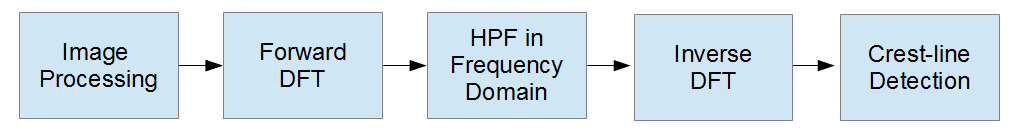
\includegraphics[width=\linewidth]{figures/flow_dft}
 	\caption{The process flow of the frequency domain approach. The images are first preprocessed, then translated into the frequency domain using the standard 2D discrete Fourier Transform. A high-pass filter is applied to the frequency domain to extract highest frequencies (which are assumed to contain dune crest-lines), and the inverse DFT is applied to return to the spacial domain. Crest-line detection can then be applied to the resulting image. }
 	\label{fig:flow_dft}
 \end{figure}

In this application, the features we desire to extract are the dune crest-lines, which in the spacial domain are edges. In the frequency domain, the crest-lines may belong to some of the higher frequencies (or possibly a subset of the frequency spectrum). The shifted frequency domain output of the DFT is shown in Figure \ref{fig:DFT_processing}.

From the frequency domain, dominant frequencies can be extracted by searching for large magnitudes of frequencies Determining which frequencies to extract will be key for this application. More research needs to be done on how to extract features from the frequency domain. Typically, from the dataset used, it can be shown that a dominant orientation in the frequency appears to be present in the dune-field images. From preliminary observations, the dominant orientation seems to correlate exactly which the orientation of the dune crests.

\begin{figure}
	\centering
	\begin{subfigure}{0.48\textwidth}
		\centering
		%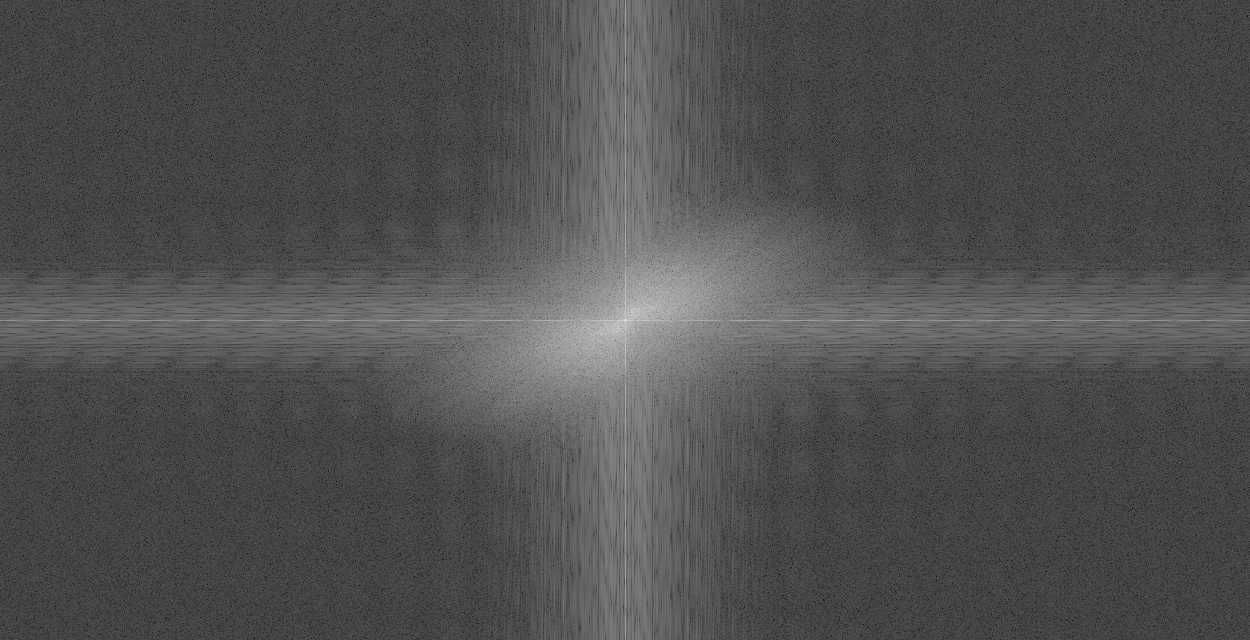
\includegraphics[width=\linewidth]{figures/DFT_spectrum}
		\caption{Skeleton Coast Frequency Domain}
		\label{fig:dft_spectrum}
	\end{subfigure}
	\begin{subfigure}{0.48\textwidth}
		\centering
		%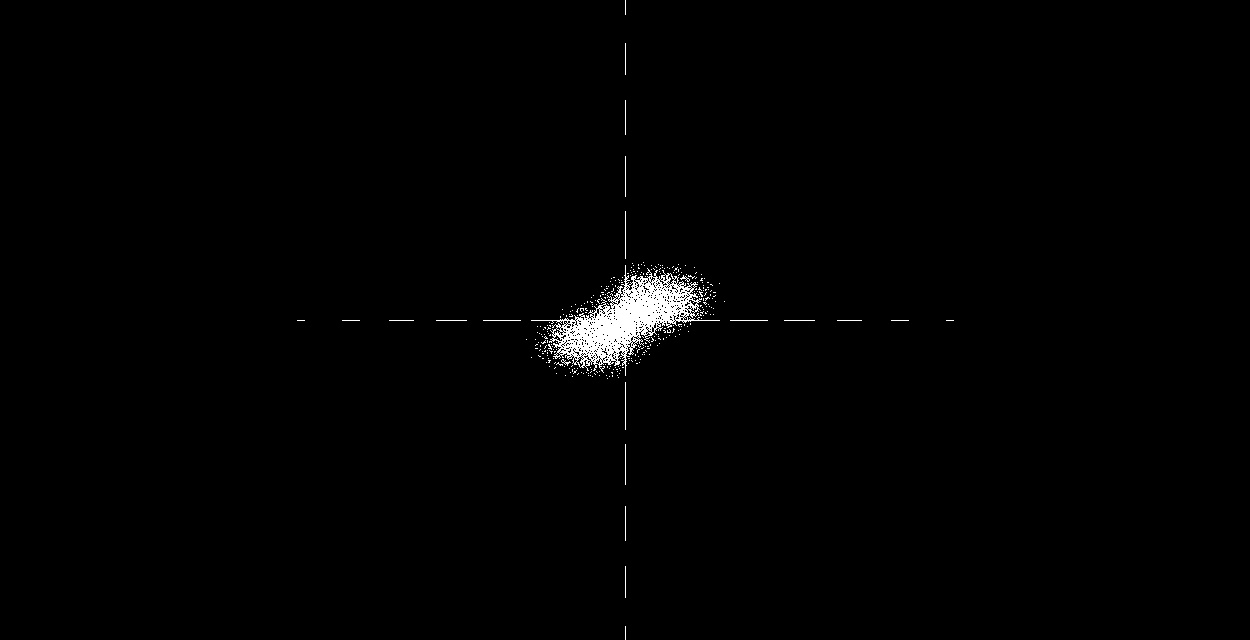
\includegraphics[width=\linewidth]{figures/DFT_spectrum_threshold}
		\caption{High Frequency Threshold}
		\label{fig:DFT_spectrum_threshold}
	\end{subfigure}
	\begin{subfigure}{0.48\textwidth}
		\centering
		%
\includegraphics[width=\linewidth]{figures/DFT_spectrum_threshold_median}
		\caption{Median Filtering}
		\label{fig:DFT_spectrum_threshold_median}
	\end{subfigure}
	\begin{subfigure}{0.48\textwidth}
		\centering
		%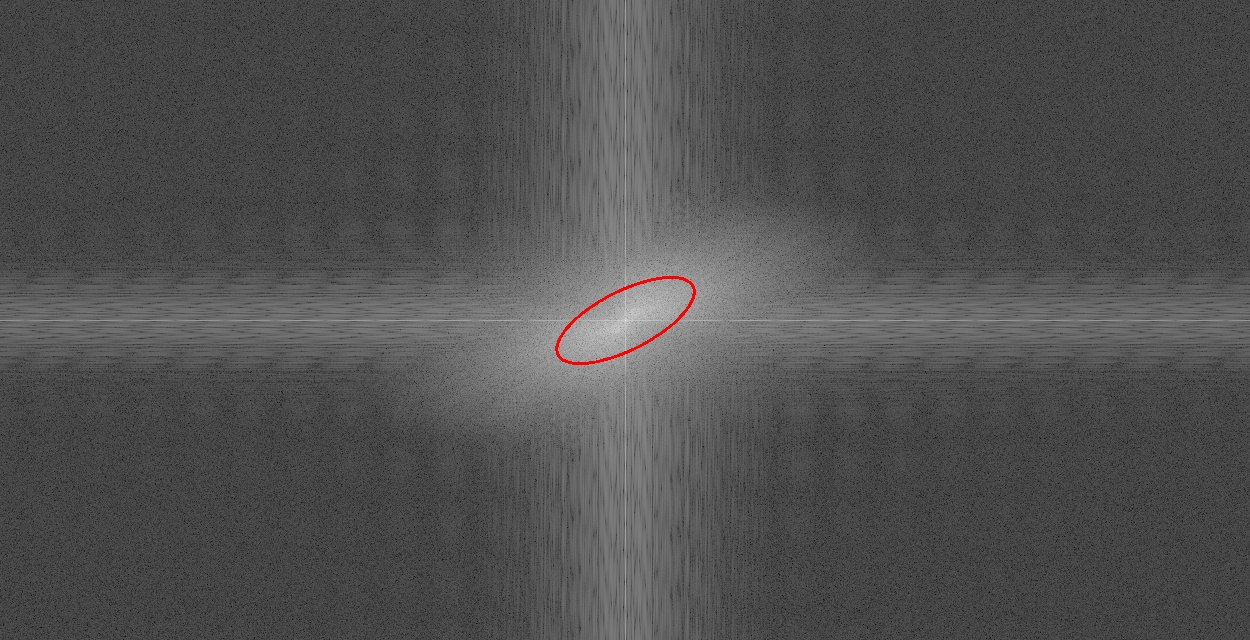
\includegraphics[width=\linewidth]{figures/DFT_spectrum_ellipsefit}
		\caption{Ellipse Fit}
		\label{fig:DFT_spectrum_ellipsefit}
	\end{subfigure}
	\begin{subfigure}{0.48\textwidth}
		\centering
		%
\includegraphics[width=\linewidth]{figures/DFT_mask}
		\caption{High-pass Filter Mask}
		\label{fig:DFT_mask}
	\end{subfigure} 
	\begin{subfigure}{0.48\textwidth}
		\centering
		%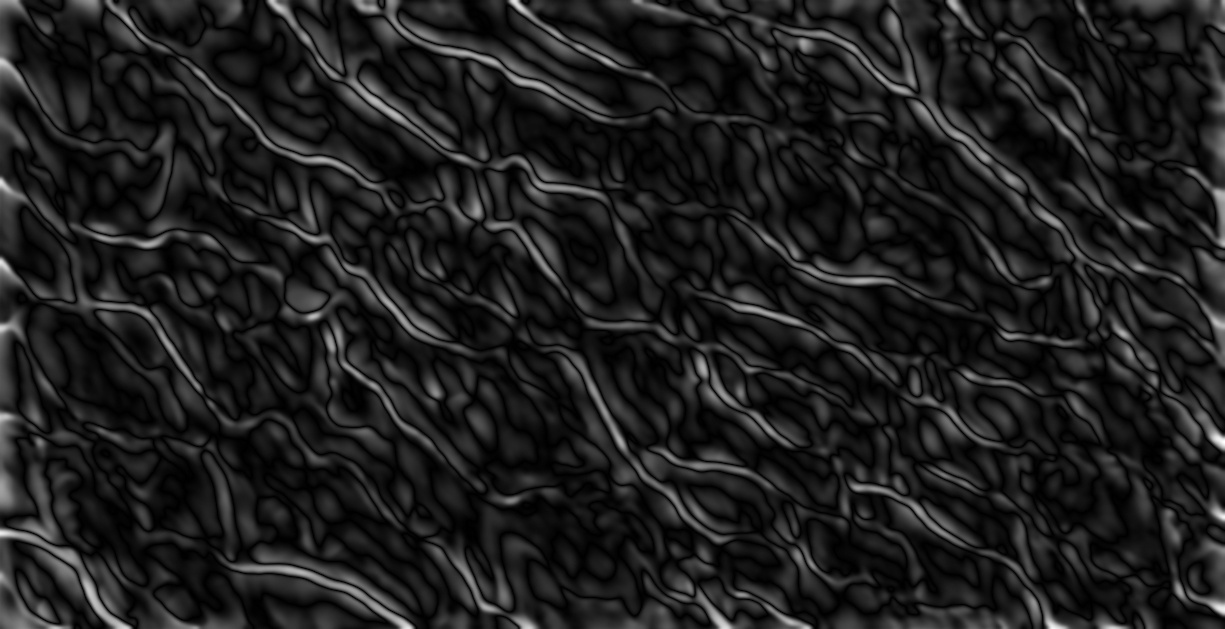
\includegraphics[width=\linewidth]{figures/DFT_HPF}
		\caption{Results of HPF on Skeleton Coast} 
		\label{fig:DFT_HPF}
	\end{subfigure} 
	\caption{Frequency spectrum processing results from the Skeleton-Coast image. \subref{fig:dft_spectrum} Log-normalized shifted frequency domain, \subref{fig:DFT_spectrum_threshold} Result of thresholding frequency domain magnitude based on average magnitude and standard deviation of the magnitudes, \subref{fig:DFT_spectrum_threshold_median} Median filtering of the binary image of the frequency domain, \subref{fig:DFT_spectrum_ellipsefit} Result of ellipse fitting of the dominant frequencies region, \subref{fig:DFT_mask} Mask used for high-pass filtering of the frequency domain, \subref{fig:DFT_HPF} Result inverse DFT of the high pass filter applied on the frequency domain. }
	\label{fig:DFT_processing}
\end{figure}

In order to determine this dominant orientation, the frequency domain magnitude image is thresholded based on the mean and standard deviation of the frequency magnitudes, as shown in Figure \ref{fig:DFT_spectrum_threshold}. Because output of this threshold is somewhat noisy, a median filter is applied to create a smooth region of for the dominant frequency (\ref{fig:DFT_spectrum_threshold_median}). The contour of the region is then extracted, which is used to fit an ellipse (\ref{fig:DFT_spectrum_ellipsefit}).

The computed ellipse's orientation appears to match the orientation of the dune gradients. The information provided by the ellipse may prove useful Fitting an ellipse is currently mainly used for determining the orientation of the gradients of the dune crests. 

There may be a better approach to extract information from the frequency domain, or other features. Currently, we use this ellipse to generate the mask for high-pass filtering. The mask shown in Figure \ref{fig:DFT_mask}) simply rejects all lower frequencies (close to the center of the spectrum), and allows all higher frequencies to pass through. 

Upon applying the mask to the frequency domain, and taking the inverse discrete Fourier Transform to return to the spacial domain, the result produces a kind of edge detection filter, where lower values could potentially be used to determine locate dune crests. The results can be seen in \ref{fig:DFT_HPF}.

Unfortunately, no further research was done on using the frequency domain. There may be some benefit in exploring this approach further in the future. The next approach presents are gradient orientation-based approach.




\subsection{Gradient Orientation-Based Approach} \label{subsec:gradient_orientation_based}
In this approach, we used knowledge learned from a previous gradient based approach, but focus on the orientation component of the gradients rather than the magnitude. The overall flow of the approach is shown in Figure \ref{fig:flow_gradient_orientation}. 

\begin{figure}[H]
	\centering
	%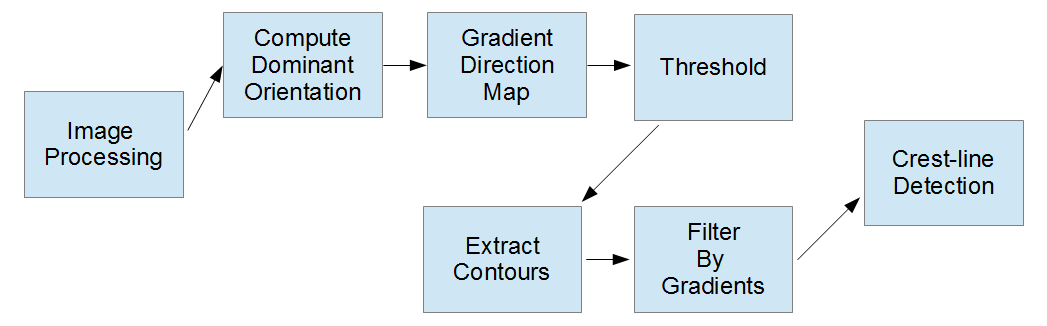
\includegraphics[width=\linewidth]{figures/flow_gradient_orientation}
	\caption{The process flow of the gradient orientation-based approach. The image is first preprocessed for optimal gradient computation, and the dominant orientation is computed. The gradient direction map is then computed and thresholded to preserve all gradients which \emph{agree} with the dominant orientation. The resulting binary image is a good candidate for contour extraction, which are subsequently filtered based on gradient orientation and magnitude. The resulting output is the detected crest-lines segments. }
	\label{fig:flow_gradient_orientation}
\end{figure}

In section \ref{subsec:edge_based_detection}, we learned that the dominant orientation of the dune field could be determined based on the derivatives of the image. In that approach, we used the gradient magnitudes to find major crest-line edges, and filtered out edges which do not \emph{agree} with the dominant orientation of the gradients. Using edges provides good localization but is prone to discontinuity of edge segments.

In contrast, this approach uses the gradient orientations of each pixel to find crest-lines. As stated previously, dunes have a bright and shaded side. Gradients in the bright and shaded sides of the dune have a tendency to point towards the crest-line.

The dominant orientation explained in section \ref{subsec:edge_based_detection} is an important feature to consider in this approach. An aspect of the dominant orientation that was not discussed previously is the fact that by definition, the dominant orientation will always point from the shaded area of the dune towards the sunlit area. This phenomenon is due to the gradient operator. Subtracting a dark pixel (lower value) from a bright pixel (larger value), results in a positive value, which in terms means that the gradients of darker pixels always point towards brighter pixels.

Given this fact, a case can be made for comparing the gradients of each pixel to the dominant orientation vector. All gradient vectors which \emph{agree} with the dominant orientation are then considered to be the shaded sides of a dune, and all gradients which \emph{disagree} with the dominant orientation are therefore part of the sunlit side of a dune. Finally the transition between areas that \emph{agree} and those that \emph{disagree} must be a good potential crest-line candidate.

The concept of \emph{agreement} can be defined mathematically using a simple dot product. Given an dominant orientation defined as a unit length vector $\hat{\delta_{\mu}}$, and the local unit length gradient vector at (i, j) defined as

\begin{equation}
\hat{\delta_{ij}} = \left\langle \frac{\delta_{x_{ij}}}{\sqrt{\delta_{x_{ij}}^2 + \delta_{y_{ij}}^2}}, \frac{\delta_{y_{ij}}}{\sqrt{\delta_{x_{ij}}^2 + \delta_{y_{ij}}^2}}\right\rangle 
\end{equation}

The \emph{agreement} measurement $D_{ij}$ then is simply the dot product:

\begin{equation}
D_{ij} = \hat{\delta_{ij}} \bullet \hat{\delta_{\mu}}
\end{equation}

Since $\hat{\delta_{ij}}$ and $\hat{\delta_{\mu}}$ are both unit-length vectors, the range possible values for $D_{ij}$ is $[-1, 1]$, where positive values represent gradients which \emph{agree} with the dominant orientation, 0 is perpendicular to the dominant orientation, and negative values \emph{disagree} with the dominant orientation. The result of the dot product computed at each pixel is shown in Figure \ref{fig:orientation_based_dot_product}, which we call the gradient direction map.

\begin{figure}
	\centering
	\begin{subfigure}{0.48\textwidth}
		\centering
		%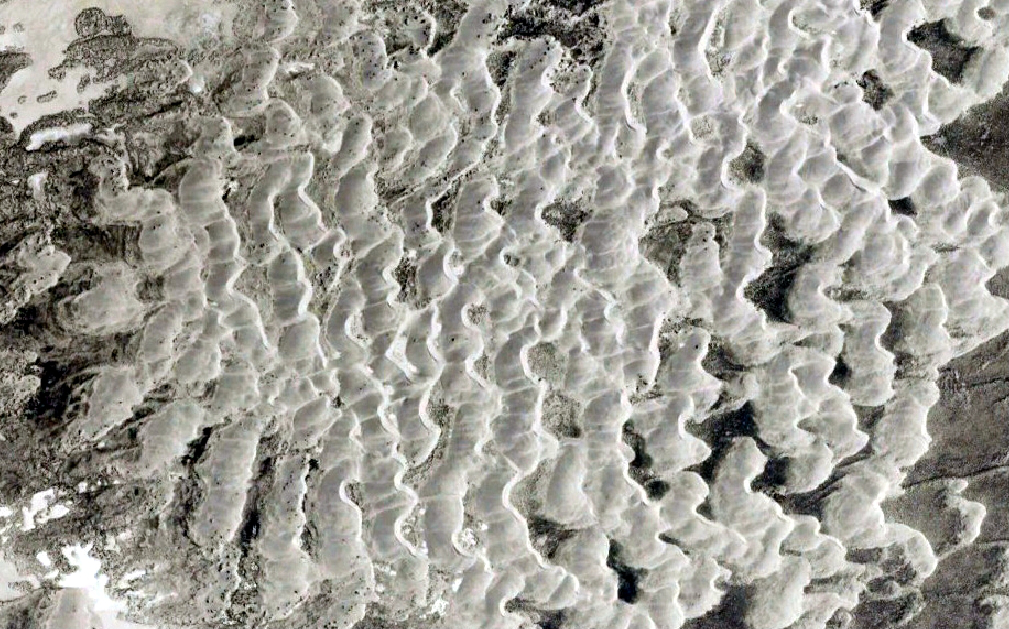
\includegraphics[width=\linewidth]{figures/wdc}
		\caption{WDC}
		\label{fig:orientation_based_wdc}
	\end{subfigure}
	\begin{subfigure}{0.48\textwidth}
		\centering
		%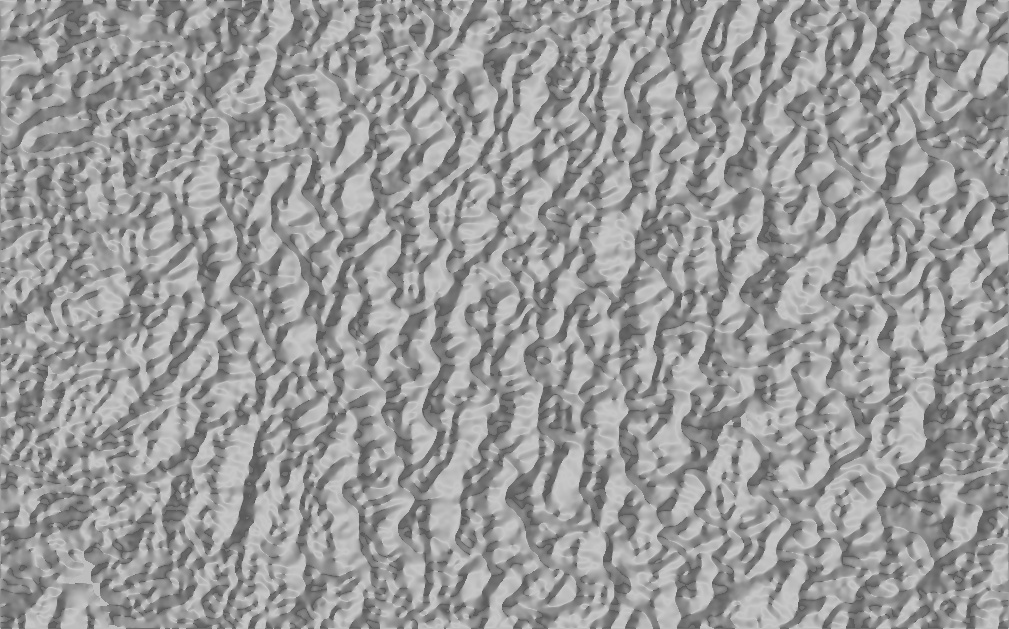
\includegraphics[width=\linewidth]{figures/dot_product}
		\caption{\emph{D}}
		\label{fig:orientation_based_dot_product}
	\end{subfigure}
	\begin{subfigure}{0.48\textwidth}
		\centering
		%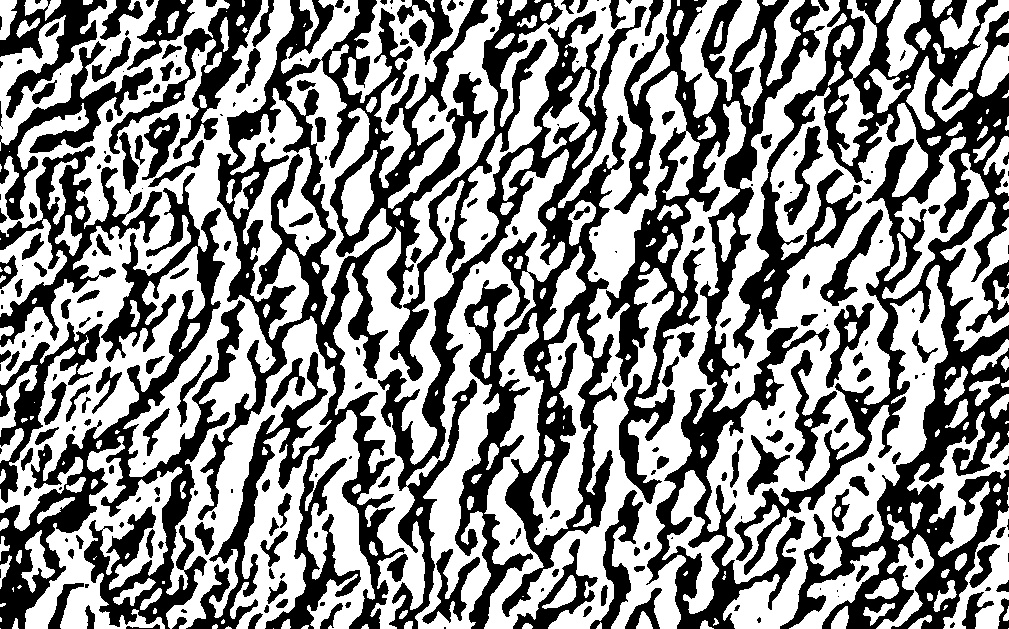
\includegraphics[width=\linewidth]{figures/threshold_dot_product}
		\caption{$\begin{cases}
				1 & D_{ij} > 0\\
				0 & otherwise
			\end{cases}$}
		\label{fig:orientation_based_threshold_dot_product}
	\end{subfigure}
	\begin{subfigure}{0.48\textwidth}
		\centering
		%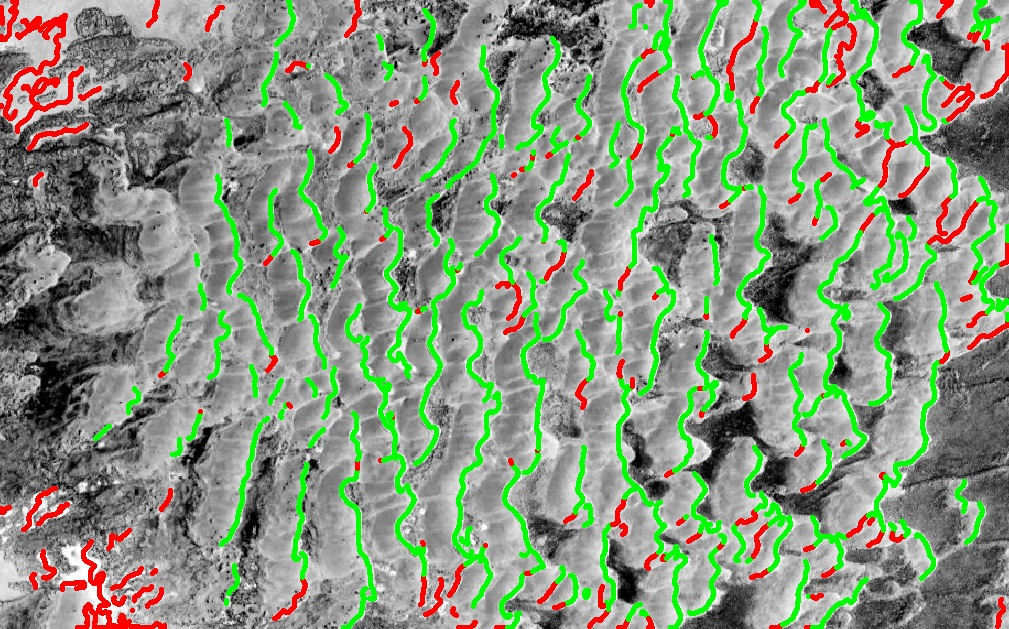
\includegraphics[width=\linewidth]{figures/method_4_results}
		\caption{Result}
		\label{fig:orientation_based_results}
	\end{subfigure}
	\caption{The gradient orientation-based approach illustrated: \subref{fig:orientation_based_wdc} The input image WDC, \subref{fig:orientation_based_dot_product} The gradient direction map \emph{D} computed by taking the dot product of the gradients at each pixel with the dominant orientation, \subref{fig:orientation_based_threshold_dot_product} thresholding the gradient direction map for all dot products greater than 0, \subref{fig:orientation_based_results} the results of crest-line detection using the gradient-orientation based method, where green lines are true positives, and red lines are false positives. }
	\label{fig:orientation_based_process}
\end{figure}

The regions produced by the gradient direction map have been shown to be typically smooth and have good continuity in this application. There appears to be a clear separation between regions in \emph{agreement} and other regions. The separation becomes even clearer when the gradient direction map is thresholded based on the dot product values. In Figure \ref{fig:orientation_based_threshold_dot_product}, a binary image of the gradient direction map is computed by thresholding all dot products above 0.

Once the gradient direction map has been thresholded, the binary image provides well defined regions which allows the use of contours to determine the crest-lines. Contours are extracted in a similar manner as presented in sections \ref{subsection:appearance_based_approach} and \ref{subsec:edge_based_detection}. The contours extracted provide good continuity of the crest-lines, but also contain many elements which are not part of the crest-line. To reject segments of the contour which are not part of the crest-lines, two techniques have been tried.

\subsubsection*{Intensity Based:}

Region contours contain crest-lines segments and non-crest-line segments. In this approach, the algorithm uses intensity values of the pixels along the contours. Segments of the contour which are on brighter regions of the image are considered to be part of the crest-lines. The use of intensity values to determine which segments of a contour are on the actual crest-line may not be an optimal solution, but has provided adequate means of rejecting many false positives.

The main benefit of this approach is that the resulting regions have sharp and defined edges along the dune crest-line, regardless of how sharp an edge is in actuality. In many cases, dunes in the same image may have some sharp edges along the crest-line while others have less defined crest-lines. Using gradient magnitude in areas with poorly defined crest-lines yields poor results, while the gradient direction maps provides a sharper edge and a better estimate of where a crest-line may be. The downside of this method is that not using the gradient magnitude results in poor localization of the actual crest-line.

\subsubsection*{Gradient Magnitude Based:} \label{subsubsec:gradient_magnitude_based_shift}

This algorithm uses the gradient values of the pixels along the contours. The assumption is that segments of the contour with larger gradients are most likely crest-line candidates. 

Using the gradient magnitudes provide much more accuracy in localizing the desired crest-lines. The gradient orientation based approach has an inherent localization problem do the the computation of the gradient orientation and size of the kernel to compute the gradients. The contours will almost always be shifted slightly away from the true crest-line as shown in Figure \ref{fig:orientation_transition_shift}.

Figure \ref{fig:orientation_transition_shift} is the exact same as the plot shown in Figure \ref{fig:kalahari_patch_plot} with the crest-line plotted, and the shift shown. The shift shown is the transition from gradients which \emph{agree} with the dominant orientation ($D_{ij} > 0$) to those which \emph{disagree} with the dominant orientation {$D_{ij} < 0$}. The shift is heavily dependent on the size of the kernel \emph{K} used to compute the gradients.

\begin{figure}
	\centering
	%\includegraphics[width=\linewidth]{figures/orientation_transition_shift}
	\caption{The cause of the shift in localization when computing the gradient direction map. The transition from gradients which \emph{agree} ($D_{ij} > 0$) with the dominant orientation almost always happens after the true crest-line due to the size of the kernel \emph{K}.}
	\label{fig:orientation_transition_shift}
\end{figure}

\begin{figure}
	\centering
	\begin{subfigure}{0.48\textwidth}
		\centering
		%\includegraphics[width=\linewidth]{figures/shift_k_9}
		\caption{$K=9$}
		\label{fig:shift_k_9}
	\end{subfigure}
	\begin{subfigure}{0.48\textwidth}
		\centering
		%\includegraphics[width=\linewidth]{figures/shift_k_21}
		\caption{$K=21$}
		\label{fig:shift_k_21}
	\end{subfigure}
	\caption{Effects of \emph{K} on the orientation-based approach. In \subref{fig:shift_k_9} a \emph{K} value of 9 is used, which results in better localization at the cost of noisier results, \subref{fig:shift_k_21} a \emph{K} value of 21 produces much smoother results but poor localization. }
	\label{fig:effect_k}
\end{figure}

The contours detected will inevitably land on the orientation transition. As shown in Figure \ref{fig:effect_k}, the parameter \emph{K} will have a tendency to shift the contour lines towards the dominant orientation. In order to improve localization, the contours must be shifted towards to nearest gradient magnitude peak. 

Two methods can be used to shift contours towards the crest-lines. Since the shift is simply dependent on the parameter \emph{K}, a fixed shift can be applied in the opposite direction of the dominant orientation. This approach may be adequate if localization is not critical, but results produced are generally less accurate.

A better solution is to search in the opposite direction of the dominant orientation for the nearest gradient magnitude peak. Each point on the contour can then be shifted by the computed distance to each gradient peak.

\subsubsection*{Parameter Effects}

For this approach, there are relatively few parameters to optimize. The main parameters are:

\begin{enumerate}
	\item The value of \emph{K}, which determines the size of the kernel which computes the gradients. The effects of varying this parameter are shown in Figure \ref{fig:effect_k}. Choosing the appropriate value for \emph{K} depends largely on the scale of the provided image, size and spacing of the dune crests. Larger kernels typically produce smoother results as shown in \ref{fig:shift_k_21}, but result in poor localization.
	\item  The value of \emph{R}, which determines the intensity or gradient magnitude value threshold for rejecting false positives. This is the main value used to determine the the appropriate level of detection. Lower threshold values typically increase the detection rates and false positive rates.
	\item The minimum segment length value, which determines the minimal allowable length for the detected segments. This parameter depends largely on the scale or resolution of the image, and the desired precision of the crest-line detection. Segments which are shorter than the minimum segment length are assumed to be noise, and are filtered out.
	\item The threshold value for the dot product, which determines how closely edges must match the dominant orientation. A value of 0 appears to be adequate in most cases, but it could be adjusted to suit the needs of the application.
\end{enumerate}

Overall, using the orientation information has merit and provides valuable information for crest-line detection. The approach is used and further improved in the approach presented in section \ref{subsec:mixed_ml_gradient_approach}. The next approach presents a traditional machine learning centric approach.



\subsection{Machine Learning Approach} \label{subsec:machine_learning_approach}

In the machine learning approach, the goal is to teach a classifier to recognize crest-lines vs non-crest-lines. A similar approach was implemented in \cite{2006_automated_classification_landform_elements,2007_Machine_Learning_tools_automatic_mapping_mars,2013_sar_image_automated_detection_dune_area,BandeiraMarques,2011_neural_network_based_dunal_landform_mapping,vaz_object_based_dune_analysis}. The goal of this approach is to create a machine learning model using a training dataset, then generate the response map which is the response of the model at each pixel in a given image. Ideally, the responses are high at pixels which contain crest-lines, and low everywhere else. The response map can be thresholded and local maximums can be traced in order to retrieve the crest-lines. The overall flow is illustrated in Figure \ref{fig:flow_ml}.

\begin{figure}[H]
	\centering
	%\includegraphics[width=\linewidth]{figures/flow_ml}
	\caption{The process flow of the machine learning approach. The image is first preprocessed, and some training data (samples of crest-lines and non-crest-lines) is reserved to construct the machine learning model. SIFT features are extracted from the training data to train the model to recognize crest-lines. With the model trained, SIFT feature descriptors are computed at each pixel of the remaining test images and are inputted into the trained model to generate the response map. Finally, the local maxima of the response map are detected in order to extract the crest-lines. }
	\label{fig:flow_ml}
\end{figure}

The first step of the process is to appropriately separate the data into training, validation, and test sets in order accurate report the performance of the method. 

\subsubsection{Dataset Creation} \label{subsubsec:dataset_creation}

Machine learning techniques typically require training data to construct the model in order to reliably solve classification problems. This method of training is called supervised learning (\cite{foundations_machine_learning_book,machine_learning_book}). For crest-line detection, we therefore need to split our data into two classes: crest-lines and non-crest-lines. 

For each class, the data also needs to be separated into three sets for training, validation and testing. 

\begin{description}
	\item [Training] The training set is used to construct the model to learn the task at hand.
	\item [Validation] The validation set is used to evaluate the effectiveness of the trained model. Based on the results produced on the validation set, the model parameters can be tuned to produce better results on the validation data.
	\item [Testing] The test set is an independent set used to report the true performance of the model.
\end{description}

In order to build the model for crest-line classification, the first step is to collect the data to build each set. In this application, our datasets included the ground truth for each image set. The ground truth is essentially a binary image with the labeled crest-lines. 

To construct an appropriate dataset for the approach, the set of images is first split into the training/validation and test sets. Half of the images are reserved for testing, and the remaining half is used to training and validation. From the set of training images, the ground truth images are used to extract locations of crest-lines and non-crest-lines. For each image, pixel positions are chosen randomly, if the ground truth at the position contains a crest-line, the pixel location is added to the crest-line set, otherwise it is added to the non-crest-line set. The sampling is optimized so that \emph{N} samples are chosen for each class.

The resulting output is that each training image now has \emph{N} samples of crest-lines, and \emph{N} samples of non-crest-lines. The next step in the process flow is to extract features from each of these samples, which will be used to feed into the model for training and validation.

\subsubsection{Feature Descriptor Extraction} \label{subsubsec:feature_descriptor_extraction}

Once sample locations of crest-lines and non-crest-lines have been selected, descriptors need to be extracted from each sample location. A descriptor is typically a vector of values which describes the local neighborhood around a pixel location (\cite{lowe_sift_paper,1994_good_features_to_track,1998_feature_detection,2007_invariant_features_survey}). The range of possible descriptor types is almost limitless. Descriptors can range from simple pixel values in an image patch, to gradient information, to more sophisticated descriptors such as HOG (Histogram of Oriented Gradients \cite{2007_hog_human_detection}), LBP (Local Binary Pattern \cite{1994_lbp_paper,1996_lbp_paper}), Haar Features (\cite{2001_viola_jones_paper}), SURF (Speeded Up Robust Features \cite{2006_surf}), SIFT (Scale Invariant Feature Transform \cite{lowe_sift_paper}), and many more.

As part of this research, many of those types of features have been investigated. However, the SIFT descriptor has been shown to provide the best overall results. One downside of the SIFT descriptor is the computational requirements of extracting and matching the descriptors. The main reason is the size of a standard SIFT descriptor, which is a vector of 128 floating point values, and becomes computational significant as the number of data samples increase. Despite this downside, SIFT is still an appropriate option since there are no real-time requirements in this application.

\begin{figure}
	\centering
	%\includegraphics[width=\linewidth]{figures/sift-descriptor}
	\caption{The SIFT descriptor explained. The image patch is split into a 4 by 4 grid, where each cell contains a histogram of gradients of eight directions. The result is a single vector of 128 floating point values. Source of the image: \underline{http://www.vlfeat.org/api/sift.html}}
	\label{fig:sift_descriptor}
\end{figure}

The SIFT descriptor, originally proposed in \cite{lowe_sift_paper} has been a standard in computer vision applications for over a decade. SIFT features extract a scale and rotation (and possibly affine) invariant region around a point of interest, and applies the descriptor to it. The descriptor is computed by splitting the scale invariant region around the point of interest in a 4 by 4 cell grid. In each cell, the histogram of gradients of 8 directions as shown in Figure \ref{fig:sift_descriptor}. The histogram in each cell is then concatenated into a single vector of 128 floating point values, and \emph{L2} normalization is applied to normalize the vector to unit length.   

In this application, the descriptor is applied to each pixel on the image, therefore there is no need for point of interest detection. To compute the SIFT descriptor, the scale and orientation of the local feature is needed. The scale in our research is ignored and is replaced by using a fixed-size window around every pixel. On the other hand, the orientation is calculated using the gradients at the local pixel location. In future work, there could be some improvements to results by computing the local scale and computing the orientation at the computed scale. Some work was done on this, but no significant improvement was noticed.

After computing the descriptor for each crest-line and non-crest-line training/validation and test samples, the classifier model can then be constructed, optimized, and validated.

\subsubsection{Supervised Learning of the Crest-line Classifier Model} \label{subsubsec:supervised_learning_classifiers}

The supervised learning method to build a classifier requires a dataset of labeled samples. Typically, each training sample is an input vector of values, with an expected output response. In this application, the input vectors are the features extracted, such as SIFT. The output response would either be a crest-line (assigned a response value of 1), or a non-crest-line (assigned a response value of -1).

The dataset of training data and their expected responses are fed into the classifier which attempts to fit a model or estimate an optimal function which separates the classes (crest-line versus non-crest-line) for the given input.

There are many different kinds of classifiers in machine learning: Bayesian, decision trees, artificial neural networks, Support Vector Machines, and many more (\cite{book_artificial_intelligence_modern_approach,2003_tackling_poor_assumptions_naive_bayes,1987_simplifying_decision_trees,1943_logical_calculus_ideas_immanent_nervous_activity,book_organization_of_behavior,1975_beyond_regression_prediction_analysis,1995_support_vector_networks,1995_support_vector_clustering}). As part of this research, we studied the various classifiers, notably SVM and Gradient Boosted Trees (\cite{1999_gradient_boosting_machine,1999_stochastic_gradient_boosting}) which provided the best performance with the SIFT features for crest-line recognition.

To train the classifier, the dataset extracted (explained in section \ref{subsubsec:dataset_creation}) of \emph{N} crest-line samples and \emph{N} non-crest-line samples are used. Many of the classifiers have free parameters to optimize, therefore a \emph{K-Fold} validation is used to construct the optimal classifier. 

\emph{K-Fold} validation is the process of splitting the data into \emph{K} folds, where one fold is used for validation and the remaining are used to train. The validation set is used to analyze results of samples not seen by the trained model, validating the reliability of the model. Typically, the process is repeated for each fold to ensure proper data representation. This process produces an optimal solution for the model while minimizing over-fitting to the training data. Over-fitting is a concept in machine learning which is defined as over learning the training data which results in weaker performance on validation and test examples (\cite{the-problem-of-overfitting,neural-network-studies-overfitting-overtraining,over-fitting-model-selection-bias}).

For this application, four main classifiers were tested: SVM, Normal Bayes, Random Trees, and Gradient Boosted Trees, all provided within the OpenCV framework \cite{opencv_library}. Once the models have been trained, they are tested using a test dataset. The results of the training of these classifiers are shown in section \ref{subsec:results-and-discussion}.

With the models recognizing crest-lines versus non-crest-lines, the next step is to construct a response map at each pixel of the images.

\subsubsection{Response Maps} \label{subsubsec:response_maps}

Response maps are images where each pixel values represent a response to a certain function. In the case of this method, the SIFT descriptor is first computed at each pixel and then used as an input for the trained classifier. Since the classifier was trained to output 1 (for crest-lines) or -1 (for non-crest-lines), the range of response values is then $[-1, 1]$. The resulting image is the response map of candidate crest-line.

The response map therefore produces an image where bright regions are likely crest-line candidates, and darker regions can be filtered out using a simple threshold. The two main classifiers which produced generally better results are the Support Vector Machines and the Gradient Boosted Trees. 

The results of the SVM classifier are shown in Figure \ref{fig:SVM_response_results}. On the left are shown the response maps for the SVM classifier (defined as \emph{R}), and on the right are the thresholded results overlapped on top of the image. This is accomplished by simply thresholding the response map \emph{R} for all pixels $(i,j)$ which are $R_{i,j} > 0$. 

The results shown are acceptable but have a tendency to be a bit noisier. There are noticeable breaks in the results, which are especially visible in Figures \ref{fig:kalahari_SVM_response_overlay} and \ref{fig:SkeletonCoast_SVM_response_overlay}. Additionally, as shown in the results Table \ref{tab:svm_training_test_results}, the SVM classifier seems to over fit the training data slightly. 
\begin{figure}[H]
	\centering
	\begin{subfigure}{0.48\textwidth}
		\centering
		%\includegraphics[width=\linewidth]{figures/KalahariSVMResponse}
		\caption{Kalahari Response Map (SVM)}
		\label{fig:kalahari_SVM_response}
	\end{subfigure}
	\begin{subfigure}{0.48\textwidth}
		\centering
		%\includegraphics[width=\linewidth]{figures/KalahariSVMResults1}
		\caption{ Kalahari $R_{i,j} > 0$}
		\label{fig:kalahari_SVM_response_overlay}
	\end{subfigure}
\end{figure}
\begin{figure}[H]
	\ContinuedFloat
	\centering
	\begin{subfigure}{0.48\textwidth}
		\centering
		%\includegraphics[width=\linewidth]{figures/NamibSVMResponse}
		\caption{Namib Response Map (SVM)}
		\label{fig:namib_SVM_response}
	\end{subfigure}
	\begin{subfigure}{0.48\textwidth}
		\centering
		%\includegraphics[width=\linewidth]{figures/NamibSVMResults1}
		\caption{ Namib $R_{i,j} > 0$}
		\label{fig:namib_SVM_response_overlay}
	\end{subfigure}
\end{figure}
\begin{figure}[H]
	\ContinuedFloat
	\centering
	\begin{subfigure}{0.48\textwidth}
		\centering
		%\includegraphics[width=\linewidth]{figures/SimpsonSVMResponse}
		\caption{Simpson Response Map (SVM)}
		\label{fig:simpson_SVM_response}
	\end{subfigure}
	\begin{subfigure}{0.48\textwidth}
		\centering
		%\includegraphics[width=\linewidth]{figures/SimpsonSVMResults1}
		\caption{ Simpson $R_{i,j} > 0$}
		\label{fig:simpson_SVM_response_overlay}
	\end{subfigure}
\end{figure}
\begin{figure}[H]
	\ContinuedFloat
	\centering
	\begin{subfigure}{0.48\textwidth}
		\centering
		%\includegraphics[width=\linewidth]{figures/SkeletonCoastSVMResponse}
		\caption{Skeleton Coast Response Map (SVM)}
		\label{fig:SkeletonCoast_SVM_response}
	\end{subfigure}
	\begin{subfigure}{0.48\textwidth}
		\centering
		%\includegraphics[width=\linewidth]{figures/SkeletonCoastSVMResults1}
		\caption{ Skeleton Coast $R_{i,j} > 0$}
		\label{fig:SkeletonCoast_SVM_response_overlay}
	\end{subfigure}
\end{figure}
\begin{figure}[H]
	\ContinuedFloat
	\centering
	\begin{subfigure}{0.48\textwidth}
		\centering
		%\includegraphics[width=\linewidth]{figures/WDCSVMResponse}
		\caption{WDC Response Map (SVM)}
		\label{fig:WDC_SVM_response}
	\end{subfigure}
	\begin{subfigure}{0.48\textwidth}
		\centering
		%\includegraphics[width=\linewidth]{figures/WDCSVMResults1}
		\caption{ WDC $R_{i,j} > 0$}
		\label{fig:WDC_SVM_response_overlay}
	\end{subfigure}
\end{figure}
\begin{figure}[H]
	\ContinuedFloat
	\centering
	\begin{subfigure}{0.48\textwidth}
		\centering
		%\includegraphics[width=\linewidth]{figures/WhiteSandsSVMResponse}
		\caption{White Sands Response Map (SVM)}
		\label{fig:WhiteSands_SVM_response}
	\end{subfigure}
	\begin{subfigure}{0.48\textwidth}
		\centering
		%\includegraphics[width=\linewidth]{figures/WhiteSandsSVMResults1}
		\caption{ White Sands $R_{i,j} > 0$}
		\label{fig:WhiteSands_SVM_response_overlay}
	\end{subfigure}
	\caption{Results of the Support Vector Machine classifier training for crest-line identification for the Terrestrial dataset shown in Figure \ref{fig:terrestrial_dataset}. On the left is the response map (the output response of the SVM classifier using the SIFT features at each pixel). On the right, the thresholded the crest-line responses ($R_{i,j} > 0$) of the response map are overlapped on the original image. }
	\label{fig:SVM_response_results}
\end{figure}

Alternatively, the Gradient Boosted Trees classifiers seems to produce slightly smoother results. The results of the Gradient Boosted Trees classifier training are shown in Table \ref{tab:boosted_trees_training_test_results}. In Figure \ref{fig:gbt_response_results}, the response maps produced by the GBT classifier are shown, similar to Figure \ref{fig:SVM_response_results}. It is clear that the resulting response maps are generally better than the SVM model.

\begin{figure}[H]
	\centering
	\begin{subfigure}{0.48\textwidth}
		\centering
		%\includegraphics[width=\linewidth]{figures/KalahariGBTResponse}
		\caption{Kalahari Response Map (GBT)}
		\label{fig:kalahari_gbt_response}
	\end{subfigure}
	\begin{subfigure}{0.48\textwidth}
		\centering
		%\includegraphics[width=\linewidth]{figures/KalahariGBTResults1}
		\caption{ Kalahari $R_{i,j} > 0$}
		\label{fig:kalahari_gbt_response_overlay}
	\end{subfigure}
\end{figure}
\begin{figure}[H]
	\ContinuedFloat
	\centering
	\begin{subfigure}{0.48\textwidth}
		\centering
		%\includegraphics[width=\linewidth]{figures/NamibGBTResponse}
		\caption{Namib Response Map (GBT)}
		\label{fig:namib_gbt_response}
	\end{subfigure}
	\begin{subfigure}{0.48\textwidth}
		\centering
		%\includegraphics[width=\linewidth]{figures/NamibGBTResults1}
		\caption{ Namib $R_{i,j} > 0$}
		\label{fig:namib_gbt_response_overlay}
	\end{subfigure}
\end{figure}
\begin{figure}[H]
	\ContinuedFloat
	\centering
	\begin{subfigure}{0.48\textwidth}
		\centering
		%\includegraphics[width=\linewidth]{figures/SimpsonGBTResponse}
		\caption{Simpson Response Map (GBT)}
		\label{fig:simpson_gbt_response}
	\end{subfigure}
	\begin{subfigure}{0.48\textwidth}
		\centering
		%\includegraphics[width=\linewidth]{figures/SimpsonGBTResults1}
		\caption{ Simpson $R_{i,j} > 0$}
		\label{fig:simpson_gbt_response_overlay}
	\end{subfigure}
\end{figure}
\begin{figure}[H]
	\ContinuedFloat
	\centering
	\begin{subfigure}{0.48\textwidth}
		\centering
		%\includegraphics[width=\linewidth]{figures/SkeletonCoastGBTResponse}
		\caption{Skeleton Coast Response Map (GBT)}
		\label{fig:SkeletonCoast_gbt_response}
	\end{subfigure}
	\begin{subfigure}{0.48\textwidth}
		\centering
		%\includegraphics[width=\linewidth]{figures/SkeletonCoastGBTResults1}
		\caption{ Skeleton Coast $R_{i,j} > 0$}
		\label{fig:SkeletonCoast_gbt_response_overlay}
	\end{subfigure}
\end{figure}
\begin{figure}[H]
	\ContinuedFloat
	\centering
	\begin{subfigure}{0.48\textwidth}
		\centering
		%\includegraphics[width=\linewidth]{figures/WDCGBTResponse}
		\caption{WDC Response Map (GBT)}
		\label{fig:WDC_gbt_response}
	\end{subfigure}
	\begin{subfigure}{0.48\textwidth}
		\centering
		%\includegraphics[width=\linewidth]{figures/WDCGBTResults1}
		\caption{ WDC $R_{i,j} > 0$}
		\label{fig:WDC_gbt_response_overlay}
	\end{subfigure}
\end{figure}
\begin{figure}[H]
	\ContinuedFloat
	\centering
	\begin{subfigure}{0.48\textwidth}
		\centering
		%\includegraphics[width=\linewidth]{figures/WhiteSandsGBTResponse}
		\caption{White Sands Response Map (GBT)}
		\label{fig:WhiteSands_gbt_response}
	\end{subfigure}
	\begin{subfigure}{0.48\textwidth}
		\centering
		%\includegraphics[width=\linewidth]{figures/WhiteSandsGBTResults1}
		\caption{ White Sands $R_{i,j} > 0$}
		\label{fig:WhiteSands_gbt_response_overlay}
	\end{subfigure}
\end{figure}
\begin{figure}[H]
	\ContinuedFloat
	\centering
	\caption{Results of the Gradient Boosted Tree classifier training for crest-line identification for the Terrestrial dataset shown in Figure \ref{fig:terrestrial_dataset}. On the left is the response map (the output response of the GBT classifier using the SIFT features at each pixel). On the right, the thresholded the crest-line responses ($R_{i,j} > 0$) of the response map are overlapped on the original image. }
	\label{fig:gbt_response_results}
\end{figure}

With the classifier model trained and the response maps generated, crest-lines can be extracted from the maps, by finding the peaks in the responses. The desired output for crest-line detection is a single pixel wide line which is smooth and contiguous. The brighter response regions tend to be thick and noisy, requiring some thinning for proper crest-line candidates to be defined. The following section will discuss the methods used to thin the responses.

\subsubsection{Crest-line Extraction: Thinning And Skeletonization}

In order to extract the desired crest-lines, the response map must be thinned. The thinning process is typically a morphological operation which reduces the thickness of a region to a single pixel width. An overview of thinning algorithms is explained in \cite{thinning-algorithms,performance-characterization-thinning,susan-new-approach-low-level-image-processing} and many other publications.

The response map should have very large values where dune crest-lines are located. The goal is to find the local maximum of the responses along ridges. The assumption is that the crest-lines should form a ridge of high response values which can be traced. As a first attempt to solve this, a recursive algorithm was created to trace the crest-lines based on the response values. The algorithm is shown in Figure \ref{fig:recursive_ridge_follow}.

\begin{figure}
	\centering
	%\includegraphics[width=\linewidth]{figures/SkeletonizationAlgorithm}
	\caption{A recursive algorithm for ridge following: On the first iteration, the algorithm is initialized using the detected anchor pixels, and begin search for each neighbor. Neighbors which are peaks along the ridge are used as anchors for the iteration. This algorithm recursively follows the ridge of the response images.}
	\label{fig:recursive_ridge_follow}
\end{figure}

The first step in the algorithm is to find \emph{anchor} points, which are starting points for the recursive algorithm. The so-called \emph{anchor} points are pixels for which the response value is larger than a defined threshold, and which have greater value than the eight neighboring pixels. Then, for each neighbor, a comparison in response value is done with their neighbors. If a neighbor has a response value greater than its two neighbors, then it is marked, and inserted into the queue of the recursive algorithm. The process is repeated until all ridge points are marked and the end of the ridge has been reached. Results of this process are shown in Figure \ref{fig:ridge_follow_results}.

\begin{figure}
	\centering
	\begin{subfigure}{0.48\textwidth}
		\centering
		%\includegraphics[width=\linewidth]{figures/kalahari}
		\caption{Kalahari Image}
		\label{fig:thinning_kalahari}
	\end{subfigure}
	\begin{subfigure}{0.48\textwidth}
		\centering
		%\includegraphics[width=\linewidth]{figures/thinning_kalahari_response}
		\caption{ Response Map (SIFT-GBT) }
		\label{fig:thinning_kalahari_response}
	\end{subfigure}
	\begin{subfigure}{0.8\textwidth}
		\centering
		%\includegraphics[width=\linewidth]{figures/thinning1_kalahari}
		\caption{ Ridge Following Thinning Algorithm }
		\label{fig:thinning1_kalahari}
	\end{subfigure}
	\begin{subfigure}{0.8\textwidth}
		\centering
		%\includegraphics[width=\linewidth]{figures/thinning1_kalahari_smooth}
		\caption{ Ridge Following with smoothing applied }
		\label{fig:thinning1_kalahari_smooth}
	\end{subfigure}
	\caption{The results of the recursive ridge following algorithm applied on the response map of the Kalahari image trained with the SIFT-GBT classifier. The results produced appear noisy and disjoint even with smoothing applied. }
	\label{fig:ridge_follow_results}
\end{figure}

Although the algorithm does thin the response maps, the results have a tendency to be noisy and disjoint. To remove noise, some Gaussian smoothing can be applied, which improves the noisy output, but does not resolve the issue of disjoint segments. Ideally, the crest-line segments should be contiguous segments of a certain specified size. One way to resolve this issue is to apply edge linking techniques such as defined in \cite{1986_canny_edge_detection}. No attempt to apply edge linking was made as part of this project, therefore more research could be done in to resolve the problem.

A better alternative is to use Skeletonization algorithms, such as explained in \cite{segmentation-free-skeletonization-grayscale-volumes,skeleton-pruning-contour-partitioning-discrete-curve-evolution,automatic-medial-axis-pruning-mapping-characteristics,fast-parallel-algorithm-thinning}. Skeletonization is the process of creating a skeleton (often referred to as a \emph{topological skeleton}) of an object or region. The goal of skeletonization is to shrink a region into a thin skeleton of the object or region. It is used in a variety of applications for its geometrical and topological properties. It enables the computation of features such as length, orientation, connectivity, and other features. 

The algorithm chosen to perform the thinning was the Zhang/Suen thinning algorithm from \cite{fast-parallel-algorithm-thinning}, due to it's simplicity and efficiency in implementation. Better algorithms may improve results of the thinning process, but for this application, the Zhang/Suen algorithm is sufficient. Before applying thinning to the response map, regions are created by thresholding the response map for all $R_{i,j} > 0$, as shown in Figure \ref{fig:thinning2_kalahari_threshold}. Then, the Zhang/Suen thinning algorithm can be applied to the binary image, shown in Figure \ref{fig:thinning2_kalahari}.

\begin{figure}
	\centering
	\begin{subfigure}{0.48\textwidth}
		\centering
		%\includegraphics[width=\linewidth]{figures/kalahari}
		\caption{Kalahari Image}
		\label{fig:thinning2_kalahari_input}
	\end{subfigure}
	\begin{subfigure}{0.48\textwidth}
		\centering
		%\includegraphics[width=\linewidth]{figures/thinning_kalahari_response}
		\caption{ Response Map (SIFT-GBT) }
		\label{fig:thinning2_kalahari_response}
	\end{subfigure}
	\begin{subfigure}{0.8\textwidth}
		\centering
		%\includegraphics[width=\linewidth]{figures/thinning2_kalahari_threshold}
		\caption{ Response Map Threshold $R_{i,j} > 0$ }
		\label{fig:thinning2_kalahari_threshold}
	\end{subfigure}
	\begin{subfigure}{0.8\textwidth}
		\centering
		%\includegraphics[width=\linewidth]{figures/thinning2_kalahari}
		\caption{ Zhang/Suen Thinning \cite{fast-parallel-algorithm-thinning} }
		\label{fig:thinning2_kalahari}
	\end{subfigure}
	\caption{The results of Zhang/Suen Thinning \cite{fast-parallel-algorithm-thinning} algorithm applied on the response map of the Kalahari image trained with the SIFT-GBT classifier. The output is much smoother and contiguous segments than the recursive ridge following method shown in Figure \ref{fig:recursive_ridge_follow}. }
	\label{fig:zhang_suen_results}
\end{figure}

The results shown in Figure \ref{fig:zhang_suen_results} are much better than the recursive algorithm shown in Figure \ref{fig:recursive_ridge_follow}. The skeletonization algorithm produces smooth contiguous segments which closely match the actual crest-lines. The final step of the method is to apply connected components to retrieve each dune segment. The length of each segment is measured and all segments which are shorter than a defined threshold can be filtered out as noise. 

The results of are shown in Table \ref{tab:machine_learning_approach_results}. The next section discusses a mixed approach, which combines elements and algorithms of the machine learning approach and previous approaches.



\subsection{Machine Learning and Gradient-Based Mixed Approach}\label{subsec:mixed_ml_gradient_approach}

The final approach which was studied as part of this research seeks to combine the concepts discussed in the previous approaches. From section \ref{subsection:appearance_based_approach}, the use of contours to retrieve contiguous segments is used. The dominant orientation calculation, defined in section \ref{subsec:edge_based_detection}, is also a key component in this approach. The use of gradient orientation maps defined in section \ref{subsec:gradient_orientation_based}, and the machine learning concepts presented in \ref{subsec:machine_learning_approach} are also utilized to maximize performance of crest-line detection.

\begin{figure}[H]
	\centering
	%\includegraphics[width=\linewidth]{figures/flow_mixed}
	\caption{The process flow of the machine learning and gradient-based mixed approach. The image is first preprocessed, and the machine learning model training is identical to the approach presented in \ref{subsec:machine_learning_approach}. Simultaneously, the dominant orientation is computed on the images, the gradient direction map is extracted, which is thresholded based on the dot product, and contours are extracted (in similar fashion to the approach explained in \ref{subsec:gradient_orientation_based}). Finally, the contours are filtered based on the response map, resulting in the detected crest-lines. }
	\label{fig:flow_mixed}
\end{figure}

As usual, each image is preprocessed to remove noise and enhance the image quality. From the processed images, a set of sample points of crest-lines and non-crest-lines are chosen randomly from a set of training data, as explained in section \ref{subsubsec:dataset_creation}. As we learned in sections \ref{subsubsec:feature_descriptor_extraction}, \ref{subsubsec:supervised_learning_classifiers}, and \ref{subsubsec:response_maps}, the features are extracted (SIFT), the classifier is trained (Gradient Boosted Trees), and the response map is created. The process of creating the response map is identical to the previous section, which is used to improve the localization of crest-lines.

\subsubsection{Gradient Orientation Crest-line Extraction}

In this process, extracting crest-line candidates is done using the method presented in section \ref{subsec:gradient_orientation_based}. To reiterate, the gradient orientation method computes the dominant orientation of the dune field, and computes the dot product of the gradients at each pixel with the computed dominant orientation, as shown in Figure \ref{fig:gradient_orientation_map_kalahari}. This produces an image where each pixels measures the \emph{agreement} with the dominant dune field orientation.  

\begin{figure}
	\centering
	\begin{subfigure}{0.48\textwidth}
		\centering
		%\includegraphics[width=\linewidth]{figures/kalahari}
		\caption{Kalahari Image}
		\label{fig:gradient_orientation_kalahari_input}
	\end{subfigure}
	\begin{subfigure}{0.48\textwidth}
		\centering
		%\includegraphics[width=\linewidth]{figures/gradient_direction_image}
		\caption{ Gradient Orientation Map ($D_{i,j}$) }
		\label{fig:gradient_orientation_map_kalahari}
	\end{subfigure}
	\begin{subfigure}{0.8\textwidth}
		\centering
		%\includegraphics[width=\linewidth]{figures/gradient_direction_thresholded_image}
		\caption{ Threshold for $D_{ij} > 0$ }
		\label{fig:threshold_gradient_orientation_map_kalahari}
	\end{subfigure}
	\caption{ Computing the Gradient Orientation Map \subref{fig:gradient_orientation_map_kalahari} ($D_{i,j}$) for the Kalahari image \subref{fig:gradient_orientation_kalahari_input}. The map is thresholded for all gradients which agree with the dominant orientation ($D_{ij} > 0$) in \subref{fig:threshold_gradient_orientation_map_kalahari}. The result produces smooth contiguous regions which contain candidate crest-lines. }
	\label{fig:gradient_orientation_map}
\end{figure}

The image produced, named the gradient orientation map, is thresholded resulting in a binary image containing regions which crest-line candidates. From the binary image, contours can be extracted from the regions using the same method shown in sections \ref{subsection:appearance_based_approach} and \ref{subsec:gradient_orientation_based}. The contours are typically smooth and contiguous, but result in poor localization. Also, there are two sets of contour around the regions. The goal is to therefore filter out one side of the contours, keeping only segments which land on the crest-line.

An additional step done in this approach is to improve the localization of the crest-lines based on the response map.

\subsubsection{Localization Improvement of Crest-line Segments}

As stated previously, the localization of the candidate crest-line contours do not land exactly on the crest-line ridges. We discussed in section \ref{subsubsec:gradient_magnitude_based_shift} the issue of localization of the contours, the cause of which is illustrated in Figure \ref{fig:orientation_transition_shift}. The shift explained in those sections was even more pronounced with larger values of \emph{K} (the size of the kernel used to compute the gradients), as shown in Figure \ref{fig:effect_k}. 

\begin{figure}
	\centering
	\begin{subfigure}{0.48\textwidth}
		\centering
		%\includegraphics[width=\linewidth]{figures/contour_binary_overlap}
		\caption{Kalahari Overlapped with Figure \ref{fig:threshold_gradient_orientation_map_kalahari}}
		\label{fig:kalahari_shift_overlap}
	\end{subfigure}
	\begin{subfigure}{0.48\textwidth}
		\centering
		%\includegraphics[width=\linewidth]{figures/contour_location_shift}
		\caption{ Contour Shift }
		\label{fig:contour_location_shift}
	\end{subfigure}
	\caption{ Illustration of the issue of poor localization of the extracted contours. In \subref{fig:kalahari_shift_overlap}, the binary image shown in Figure \ref{fig:threshold_gradient_orientation_map_kalahari} is overlapped on top of the Kalahari image \ref{fig:gradient_orientation_kalahari_input}. In \subref{fig:contour_location_shift}, a zoomed in image patch reveals the localization issue with the contours (shown in red) from the actual crest-line (shown in green). In order to improve the localization, the contour segments must be shifted towards crest-line. The shift is applied in the direction opposite to the computed dominant orientation. }
	\label{fig:shifting_contours_to_crest_lines}
\end{figure}

To further expand on the problem, Figure \ref{fig:shifting_contours_to_crest_lines} shows the shift created from the binary image contours. In order to improve the localization of the candidate contour segments, each segment needs to be shifted towards the crest-line ridge. The result of the contour segment extraction is shown in Figure \ref{fig:gradient_direction_results_no_shift_no_filter}, clearly showing the localization issue. Two considerations must be made in order to properly shift the candidate crest-lines to the actual crest-line: the direction of the shift, and the algorithm used to shift.

Because of the way the gradient orientation map was computed, an appropriate shifting direction can be in the opposite direction of the dominant orientation, as shown in Figure \ref{fig:contour_location_shift}. There may be better solution for shifting, but using the dominant orientation makes sense in this case and generally produces good results. Since the direction of the shift is known, the next step is to find the actual crest-line ridge along the direction of the shift. The solution proposed in \ref{subsec:gradient_orientation_based} was to find the nearest gradient magnitude peak. Unfortunately, as discussed in \ref{subsec:challenges}, some crest-line gradients may be relatively weak, making localization a difficult task.

\begin{figure}
	\centering
	\begin{subfigure}{0.48\textwidth}
		\centering
		%\includegraphics[width=\linewidth]{figures/kalahari}
		\caption{Kalahari Image}
		\label{fig:kalahari_image_2}
	\end{subfigure}
	\begin{subfigure}{0.48\textwidth}
		\centering
		%\includegraphics[width=\linewidth]{figures/gradient_direction_results_no_shift_no_filter}
		\caption{Contours Extracted from Binary Image}
		\label{fig:gradient_direction_results_no_shift_no_filter}
	\end{subfigure}
	\begin{subfigure}{0.48\textwidth}
		\centering
		%\includegraphics[width=\linewidth]{figures/gradient_direction_results_no_filter}
		\caption{ After Applying Shift }
		\label{fig:gradient_direction_results_no_filter}
	\end{subfigure}
	\begin{subfigure}{0.48\textwidth}
		\centering
		%\includegraphics[width=\linewidth]{figures/gradient_direction_shift_results}
		\caption{ Filtering Based on Responses }
		\label{fig:gradient_direction_shift_results}
	\end{subfigure}
	\caption{ The process of extracting candidate crest-lines using the gradient orientation map, and the machine learning approach. The Kalahari input image shown in (a), is processed to extract contours shown in (b). A shift towards the nearest peak in response values is applied (c), and all segments which have low responses are filtered out in (d). The color scheme shown in (b-d) is true positive crest-lines detections (green), the positive identified ground truth (blue), false negatives (yellow), and false positives (red).}
	\label{fig:shifting_contours_results}
\end{figure}

Therefore, using the response map computed in the previous approach seems to be an appropriate way to resolve this problem. The response map will have larger values where crest-lines are located. So, the shift can be determined by doing a search along the opposite direction of the dominant orientation, and finding peaks in the response map. The shift can then be applied based on the computed distance, for each point along the contour segments. Smoothing can be applied in order to ensure that segments remain contiguous after the shift is applied. The results of the shift are shown in Figure \ref{fig:gradient_direction_results_no_filter}.

Once the shift has been applied to every contour segments, filtering non-crest-line segments can be done by simply removing all contour segments which fall on weak responses. After all contours have been filtered, the remaining segments can be further filtered by segment length. All segments which are too short are removed from candidate crest-line segments. The output of this process is shown in Figure \ref{fig:gradient_direction_shift_results}.

Overall, the mixed machine learning and gradient orientation based method produced excellent results in most cases but struggled on more complex dune systems. Section \ref{subsec:results-and-discussion} summarizes the results of this approach on both our dataset and the dataset provided by \cite{vaz_object_based_dune_analysis}. The next section discusses the method and metrics computed from the detected crest-lines.


\subsection{Dune Field Morphology Metrics} \label{subsec:dune-field-metrics}
The final step of the process is to extract meaningful features and metrics for researchers to study from the dune fields. This process requires a good set of detected crest-lines. The output crest-line segments extracted in the previous methods are used as input for computing the features.

There are many features metrics of interests to scientists in this field, including dune spacings, orientation, shape, size, length, bifurcations, and many more. These metrics can be used to study and understand the movements of various patterns of dunes over time in a specific area.

As part of this research, we focused mainly on orientation and spacing of dunes, and used those metrics as validations for the effectiveness of the dune detection methods. Although these metrics are not a complete evaluation of the dune field, they are sufficiently complex to provide valuable feedback for scientists.

\subsubsection{Dune Field Orientation Computation}
One may argue that the orientation of the dune field could be simply computed in the same manner as explained in section \ref{subsec:edge_based_detection}. However, a more generalized approach is preferred which computes the metrics from any set of two dimensional points, regardless of the input image. 

In order to compute the average dune field orientation from the detected points, the data must be formated appropriately. The detected crest-lines are typically a set of two dimensional points on the image. These points form lines and segments of various shapes and lengths. The simplest way to compute the orientation is to fit lines to each segments and compute the average orientation of the lines.

There are many commonly used methods to fit lines to segments. One popular method is the Hough Transform initially proposed in \cite{hough-1959-paper,hough-1962-patent,hough-duda-1972-paper}, which searches a space of parameters voting for segments which contribute to the line. The Hough transform can be generalized to many shapes suchs as circles and ellipses, but the parameter space gets much larger for complex shapes. The main drawback of the Hough transform is the computational cost of search a large parameter space.

An alternative method is the Ramer-Douglas-Peucker algorithm, proposed in \cite{ramer-1972-paper,douglas-peucker-1973-paper,douglas-hershberger-snoeyink-1992-paper}, with the implementation provided within the OpenCV (\cite{opencv_library}) framework. The method is used for simplifying or approximating any given curve to a subset of points. Thus, the dune segments can be reduced to subset of lines. The only parameter required is the allowable error in the approximation. Larger values allow more deviation, producing longer coarse approximations of the segments, while smaller values approximate the curve more closely, producing short segments which are sensitive to noise. The parameter is chosen to produce optimal results for the application.

\begin{figure}
	\centering
	\begin{subfigure}{0.48\textwidth}
		\centering
		%\includegraphics[width=\linewidth]{figures/SegmentationTestImage}
		\caption{Sample Test Image}
		\label{fig:connected_component_test_image}
	\end{subfigure}
	\begin{subfigure}{0.48\textwidth}
		\centering
		%\includegraphics[width=\linewidth]{figures/SegmentationTestResult}
		\caption{Connected Components Labeling}
		\label{fig:connected_component_test_results}
	\end{subfigure}
	
	\caption{ The connected component algorithm applied a sample test image \subref{fig:connected_component_test_image}. The results \subref{fig:connected_component_test_results} show that segments can be extracted correctly. }
	\label{fig:connected_component_test}
\end{figure}

Another critical requirement for this algorithm to work is the fact that each segment must be a single contiguous line or curve. This means that any segments extracted from the connected components algorithm (\cite{connected-components-samet-tamminen-1988-paper,connected-components-dillencourt-1992-paper}) must be sorted and organized in a list to ensure contiguous segments of points. All forks and bifurcations are detected and split into separate segments. The labeling of segment is demonstrated on a test image shown in Figure \ref{fig:connected_component_test}. The results in Figure \ref{fig:connected_component_test_results} show that these segments can be extracted and split into many single line segments. Although the algorithm may not produce optimal results, the output is sufficient for this application.

Once the segments have been extracted and sorted, the line fitting algorithm presented in \cite{ramer-1972-paper} can be applied. The result is a set of lines, which can be represented as vectors contain the position and orientation of each line. The orientation components are used to compute the average orientation of the dune field.

As explained in \cite{computing-average-orientation-of-vectors}, computing the average orientation of vectors is not as trivial as simply averaging the orientations. To illustrate the problem, the average of an angle of $350^{\circ}$ and $10^{\circ}$ would be $180^{\circ}$, when in fact a more appropriate average should be $0^{\circ}$. Averaging may produce an adequate approximation, but the von Mises distribution based method proposed in \cite{computing-average-orientation-of-vectors} typically produces much more accurate results. Therefore, this technique is used to compute the average orientation of the lines.

With the orientation of the dune field computed, the average dune distance can then be computed.

\subsubsection{Inter-Dune Distance Computation}
Computing the distance between crest-lines is a feature interesting to many researchers in the field. For simplicity, the inter-dune spacing is computed for the entire dune field image. The resulting measurement is in pixels in our case, but, if the scale of the satellite image is known (meters per pixels), then the measurement can be easily converted to a real world measurement. There are many ways to compute the inter-dune distance, but in this approach the simplest way was used, shown in Figure \ref{fig:inter-dune-distance-computation}. 

\begin{figure}
	\centering
	%\includegraphics[width=\linewidth]{figures/DuneMetrics}
	\caption{ Computing the inter-dune distance using the average orientation. Once the average orientation has been computed, the inter-dune distance can be computed by measuring the distance between segments along an orthogonal axis to the average orientation.}
	\label{fig:inter-dune-distance-computation}
\end{figure}

Using the binary image of the extracted dune crest-lines, and the average orientation computed, an iterative approach is used to measure the distance between the dunes. A search is done at each pixel along an orthogonal axis from the average orientation. When a crest-line is hit, the number of pixels traveled are counted until another dune is found. The process is repeated for the entire binary image. The lengths are averaged resulting in the average dune spacing for the entire dune field.

The results produced may not be optimal and accurate but can be used as an indicator to evaluate the effectiveness of the dune crest-line detections. The results and metrics are presented in section \ref{subsec:results-and-discussion}.











\section{Experimental Evaluation} \label{sec:experimental_evaluation}

In this section, the experiments and results are presented. First, the datasets used to conduct the experiments and test the crest-line detection methods is presented in section \ref{subsec:study-areas}. Two main datasets were used for the study:

\begin{description}[align=left]
	\item[Terrestrial Dataset] A sample dataset of various regions created and labeled by an expert in the field, specifically for this research.
	\item[Mars Dataset] The dataset from the Ganges Crater area on Mars, defined by \cite{vaz_object_based_dune_analysis}.
\end{description}

The next section discusses the evaluation used for measuring the quality of each dune crest-line detector method. The main metrics used are the Precision, Recall, and dune features presented in section \ref{subsec:dune-field-metrics}. Finally, section \ref{subsec:results-and-discussion} presents the results along with a short discussion of the methods. 

\subsection{Study Areas} \label{subsec:study-areas}

As part of this research project, two datasets were used in order to evaluate the robustness of each method. The datasets include a wide range of dune types with varying morphological properties. The data provided in each set are satellite images of dune field regions available through Google Earth and NASA datasets. Included with the images is the ground truth which has been manually labeled by experts in the research field. The ground truth consists of crest-lines for each positive dune detection. In each case, the scales of the satellite images were chosen such that the inter-dune distance appeared roughly normalized across the entire dataset. Scale selection of the images is important process for even comparison of the methods for different regions. The images are resized to an appropriate resolution for processing and even across the entire dataset.

The method described in this paper was tested on two distinct datasets: an terrestrial dataset which includes dune fields of various regions on Earth, along with the dataset provided in \cite{vaz_object_based_dune_analysis} which is located on Mars in the Ganges crater region. The same method was applied on both datasets.

\subsubsection{Terrestrial Dataset}
\label{subsec:terrestrial_dataset}
The first dataset is a small sample of a dozen satellite images from six separate desert regions on Earth (shown in Figure \ref{fig:terrestrial_dataset}). Included are the Kalahari, Namib and Skeleton Coast sand sea regions in Namibia (\cite{goudie_desert_landforms_namibia}). Also represented in this dataset are the Simpson dune field in Australia, the Winnemucca Dune Complex in Nevada, and the White Sands National Monument. A wide range of landforms types are contained within each of these regions which provides a broad study for an automated crest-line detection method. 

\begin{figure}
	\centering
	\begin{subfigure}{\textwidth}
		\centering
		%\includegraphics[width=0.45\linewidth]{figures/kalahari}
		%\includegraphics[width=0.45\linewidth]{figures/kalahari_gt}
		\caption{ Kalahari }
		\label{fig:kalahari_image}
	\end{subfigure}
	\begin{subfigure}{\textwidth}
		\centering
		%\includegraphics[width=0.45\linewidth]{figures/namib}
		%\includegraphics[width=0.45\linewidth]{figures/namib_gt}
		\caption{ Namib }
		\label{fig:namib_image}
	\end{subfigure}
	\begin{subfigure}{\textwidth}
		\centering
		%\includegraphics[width=0.45\linewidth]{figures/simpson}
		%\includegraphics[width=0.45\linewidth]{figures/simpson_gt}
		\caption{ Simpson}
		\label{fig:simpson_image}
	\end{subfigure}
\end{figure}
\begin{figure}
	\ContinuedFloat
	\centering
	\begin{subfigure}{\textwidth}
		\centering
		%\includegraphics[width=0.45\linewidth]{figures/skeletoncoast}
		%\includegraphics[width=0.45\linewidth]{figures/skeletoncoast_gt}
		\caption{ Skeleton Coast}
		\label{fig:skeleton_coast_image}
	\end{subfigure}
	\begin{subfigure}{\textwidth}
		\centering
		%\includegraphics[width=0.45\linewidth]{figures/wdc}
		%\includegraphics[width=0.45\linewidth]{figures/wdc_gt}
		\caption{ Winnemucca Dune Complex }
		\label{fig:wdc_image}
	\end{subfigure}
	\begin{subfigure}{\textwidth}
		\centering
		%\includegraphics[width=0.45\linewidth]{figures/whitesands}
		%\includegraphics[width=0.45\linewidth]{figures/whitesands_gt}
		\caption{ White Sands }
		\label{fig:white_sands_image}
	\end{subfigure}
	\caption{Terrestrial dataset of six regions with respective labeled ground truth: (\ref{fig:kalahari_image}) Kalahari (Namibia), (\ref{fig:namib_image}) Namib (Namibia), (\ref{fig:simpson_image}) Simpson (Australia), (\ref{fig:skeleton_coast_image}) Skeleton Coast (Namibia), (\ref{fig:wdc_image}) Winnemucca Dune Complex (USA), and (\ref{fig:white_sands_image}) White Sands (USA)}
	\label{fig:terrestrial_dataset}
\end{figure}


The Kalahari (Figure \ref{fig:kalahari_image})sands span from the southeastern region of Namibia to South Africa. The region is a 100-200 km wide and is composed of mostly fixed dunes \cite{lancaster_linear_dunes_kalahari}. Most of the area is comprised of simple linear form dunes, although some small areas contain some compound linear dunes as well. Unlike other desert regions, the Kalahari contains areas which are well vegetated. On average, the dunes range from 2m to 15m in height, with a 150m to 250m width, and spaced from 200m to 240m. These measurements may be useful for determining the reliability of our metric calculations.

The Namib Sand Sea (Figure \ref{fig:namib_image}) region spans approximately 34,000 km of the Altantic coast of Namibia, contains some of the largest and oldest sand dunes in the world according to \cite{goodie_namib_sand_sea_ancient_desert}. High energy unimodal, bimodal and complex wind regimes create interesting dune field patterns in the Namib Sand Sea region of Namibia \cite{lancaster_winds_sand_movement_namib_sea}. These wind patterns characterize the spatial variability of the dune types, sizes, and other morphological properties of the region, making it an interesting case study for this research.

The Skeleton Coast (Figure \ref{fig:skeleton_coast_image}) dune field contains simple, locally compound, transverse and barchanoid dunes over its 2000 km\textsuperscript{2} span according to \cite{lancaster_dunes_skeleton_coast}. The dunes pattern in this region are formed due to onshore winds and surface roughness changes between the dunes and coastal plains. The dune field is roughly aligned with the coast and is characterized with a large slip face in which dunes range from 20m to 80m in height.

Another region represented in the dataset is the Simpson (Figure \ref{fig:simpson_image}) dune field in Australia. Much like the Kalahari sands in southern Africa, the Simpson dune fields contains many similar features. The areas are home to lush vegetation, and the dune field follow a mostly simple linear pattern where the dunes tend to be broad crested \cite{hesse_australian_desert_dunefields}. According to \cite{twidale_simpson_desert_australia}, some of the ridges continue unbroken for up to 200 km, where each crest measures 15m to 38m in height. The spacing between each crest varies depending on the height of the ridges. Areas with larger ridges may have one or two dunes per kilometer, while smaller ridges may have five or six dunes per kilometer. These factor make this area an interesting addition to the dataset because the scale of the images is much larger.

Also present is the Winnemucca Dune Complex (WDC, Figure \ref{fig:wdc_image}) found in the western United States, in Nevada. The WDC covers an area of roughly 900 km\textsuperscript{2} north of Winnemucca, Nevada. The most common dune type present are stabilized parabolic dunes, but barchans and transverse ridges can also be found scattered throughout the area \cite{zimbelman_eolian_deposits_western_united_states}. In fact, according to \cite{pepe_winnemucca_dune_complex}, the WDC is primarily covered by six crescentic complexes, a large sand sheet, and discontinuous sets of compound barchanbolic-parabolic dune fields. The WDC contains a complex set of repetitive sequences of dunes which varying shapes and scales, which makes it an ideal candidate for this dataset.

Finally, the last area in the dataset is the White Sands National Monument (fig. \ref{fig:white_sands_image}), located in the state of New Mexico, USA. This area boasts an interesting pattern of crescentric aeolian dunes which are formed in a systematically similar fashion to wind ripples and sub-aqueous dunes \cite{ewing_aeolian_dune_interaction_white_sands}. There are a wide range of features and properties in the White Sands dune field that merit study, such as described in \cite{ewing_aeolian_dune_interaction_white_sands}. These interactions include merging, lateral linking, defect repulsion, bed-form repulsion, off-center collision, defect creation and dune splitting. The details of these interactions are outside the scope of this research but crest-line detection may be an essential preliminary step towards extracting those features. Measuring the number of dunes, crest lengths, defect density, dune spacing, and dune height are all done manually by experts in the field. A move towards an automated process would greatly improve research efforts, and would be a helpful tool for scientist in the field.

\subsubsection{Mars Dataset}
\label{subsec:mars_dataset}
To verify the robustness of this approach, the method was also tested on another dataset which was used in \cite{vaz_object_based_dune_analysis}. The dataset provided is from the Ganges Chasms on Mars, and includes satellite images, manually labeled crest-lines, and the results of the original author's method. The provided results lay a baseline benchmark for measuring quality and accuracy of crest-line detection algorithms. In order to more easily process the dataset, the Ganges region was split into sixteen areas of equal size, as shown in Figure \ref{fig:mars_ganges_dataset}. The ground truth included was not validated for correctness, the labeled data was used as-is, which may account for some errors (see Section \ref{subsec:results-and-discussion}).

\begin{figure}
	\centering
	\begin{subfigure}{\textwidth}
		\centering
		%\includegraphics[width=0.7\linewidth]{figures/ganges_regions}
		\caption{}
		\label{fig:ganges_regions}
	\end{subfigure}
	\begin{subfigure}{\textwidth}
		\centering
		%\includegraphics[width=0.45\linewidth]{figures/ganges1}
		%\includegraphics[width=0.45\linewidth]{figures/ganges1_gt}
		\caption{}
		\label{fig:ganges1_image}
	\end{subfigure}
	\caption{Ganges Chasms Mars dataset from \cite{vaz_object_based_dune_analysis} which includes (\ref{fig:ganges_regions}) 16 regions extracted, (\ref{fig:ganges1_image}) sample image from region 1 with corresponding labeled ground truth}
	\label{fig:mars_ganges_dataset}
\end{figure}


The dataset is essentially a CTX mosaic of the Ganges chasma, which spans an area of 500 km\textsuperscript{2}, and includes a wide variety of dune types and morphologies. According to \cite{fenton_aeolian_sediment_ganges_chasma_mars}, many aeolian fatures can be found in the Ganges Chasma. Sand sheets, dune fields, unidirectional features such as barchan dunes were all identified within this region. The overall structure of the Ganges dune field is a complex set of many diverging dunes, which makes it a challenging and appropriate area for testing this method. 


\subsection{Evaluation}\label{subsec:evaluation}

For each method, a number of metrics were used to evaluate the quality of each dune detector. A true positive (\emph{TP}) is defined as a positively detected crest-lines. A detection is determined to be positive if it contains a ground truth within a radius of $\epsilon$. A false positive (\emph{FP}) is defined to be a detection which is not an actual dune crest-line. A false positive occurs when a detection does not have a ground truth crest-line within a radius of $\epsilon$. A false negative (\emph{FN}) is an actual ground truth crest-line which was no identified. A false negative occurs when no detection is found within a radius of $\epsilon$.

Determining an appropriate value for $\epsilon$ affects the overall results as well. Based on the datasets used in this research, and accounting for error in labeling and image resolution, an appropriate value was chosen to be $\epsilon=10$ (pixels). If the scale of the image is known (meters per pixel), pixels can be converted to a more meaningful metric scale.

\emph{Precision} is the ratio of correct detection to overall detection. It measures how precise the detections are. It can be computed from the true positives and false positives by $P=TP/(TP+FP)$. \emph{Recall} Recall is the percentage of crest-lines identified. It can be computed from the true positives and false negatives using $R=TP/(TP+FN)$. \emph{Angular Error} The difference between the dune field average orientation computed from the detected crest-lines, and the average orientation computed from the ground truth crest-lines (in degrees), represented by $\Delta_{\theta}$. Finally, the \emph{Inter-Dune Distance Error} The difference between the dune distance computed from the detected crest-lines and the distance computed from the ground truth crest-lines (in pixels), represented by $\Delta_{d}$.

Additionally, the terrestrial dataset includes many representative regions with various dune types. There are two options for training models:
\begin{description}
	\item[Unique Model Per Region] In this approach, a machine learning model is trained for each region. The result are more accurate within each regions, but the solution is not as generalized. 
	\item[Cross-Region Model] In this approach, a single model is trained using all regions. The results produced are typically less accurate than the unique model per region approach, but provides a more generalized solution.
\end{description}

Another dataset evaluated was the Mars dataset from section \ref{subsec:mars_dataset}. Included are the results from the research done in \cite{vaz_object_based_dune_analysis}, which includes the ground truth and results. Our machine learning method was compared side-by-side with the results from \cite{vaz_object_based_dune_analysis} on each of the 16 regions sampled. The 16 regions are split half and half for training and testing respectively, where odd regions were used for training and even regions for testing. 

\subsection{Results} \label{subsec:results-and-discussion}
To recap, the machine learning approaches require the training of the models using a set of data and the model is then tested on a separate set of data. Therefore, a separate set of data was created to evaluate the performance of the machine learning approach, shown in Figure \ref{fig:terrestrial_test_dataset}.

\begin{figure}
	\centering
	\begin{subfigure}{\textwidth}
		\centering
		%\includegraphics[width=0.45\linewidth]{figures/kalahari_test}
		%\includegraphics[width=0.45\linewidth]{figures/kalahari_test_gt}
		\caption{ Kalahari Test }
		\label{fig:kalahari_test_image}
	\end{subfigure}
	\begin{subfigure}{\textwidth}
		\centering
		%\includegraphics[width=0.45\linewidth]{figures/namib_test}
		%\includegraphics[width=0.45\linewidth]{figures/namib_test_gt}
		\caption{ Namib Test }
		\label{fig:namib_test_image}
	\end{subfigure}
	\begin{subfigure}{\textwidth}
		\centering
		%\includegraphics[width=0.45\linewidth]{figures/simpson_test}
		%\includegraphics[width=0.45\linewidth]{figures/simpson_test_gt}
		\caption{ Simpson Test }
		\label{fig:simpson_test_image}
	\end{subfigure}
\end{figure}
\begin{figure}
	\ContinuedFloat
	\centering
	\begin{subfigure}{\textwidth}
		\centering
		%\includegraphics[width=0.45\linewidth]{figures/skeleton_coast_test}
		%\includegraphics[width=0.45\linewidth]{figures/skeleton_coast_test_gt}
		\caption{ Skeleton Coast Test }
		\label{fig:skeleton_coast_test_image}
	\end{subfigure}
	\begin{subfigure}{\textwidth}
		\centering
		%\includegraphics[width=0.45\linewidth]{figures/wdc_test}
		%\includegraphics[width=0.45\linewidth]{figures/wdc_test_gt}
		\caption{ Winnemucca Dune Complex Test }
		\label{fig:wdc_test_image}
	\end{subfigure}
	\begin{subfigure}{\textwidth}
		\centering
		%\includegraphics[width=0.45\linewidth]{figures/whitesands_test}
		%\includegraphics[width=0.45\linewidth]{figures/whitesands_test_gt}
		\caption{ White Sands Test }
		\label{fig:white_sands_test_image}
	\end{subfigure}
	\caption{Terrestrial test dataset of six regions with respective labeled ground truth: (\ref{fig:kalahari_test_image}) Kalahari (Namibia), (\ref{fig:namib_test_image}) Namib (Namibia), (\ref{fig:simpson_test_image}) Simpson (Australia), (\ref{fig:skeleton_coast_test_image}) Skeleton Coast (Namibia), (\ref{fig:wdc_test_image}) Winnemucca Dune Complex (USA), and (\ref{fig:white_sands_test_image}) White Sands (USA), used for evaluation of machine learning approaches. Test }
	\label{fig:terrestrial_test_dataset}
\end{figure}

The addition of the test images allows us to better evaluate the effectiveness of the various models and methods used to train the machine learning system. To train each model a set of data is collected from the both the training and test sets using the method described in section \ref{subsubsec:dataset_creation}. A set of pixels are randomly selected for each image, preserving a equal count of crest-line pixels and non-crest-line pixels. Crest-line pixels are determined using the provided ground truth. The number of pixels extracted was varied to determine the effectiveness of the model. When fewer data was used, the model could be trained very quickly but the representation of the model achieved poorer results. A larger training set provided a much better representation of crest-lines, at the cost of efficiency. The number of pixels used found to be optimal was in the range of 1000 to 5000.

As described in section \ref{subsubsec:feature_descriptor_extraction}, the features were extracted at each sampled pixel. Many feature types were used including BRIEF, ORB, BRISK, SURF, HOG, LBPH, and even using raw pixel values but the SIFT performance was far superior to all others. The traditional 128 bin SIFT descriptor vector was extracted at each pixel as the feature to use for the model.

The next consideration is the type of machine learning classifier to use for the model. Again, as described in section \ref{subsubsec:supervised_learning_classifiers}, there are many classifier options available such as Bayesian, Neural Networks, Decision Trees, Support Vector Machines.

\begin{table}
	\centering
	\caption{True positive and false positive rates results of the training process to build the crest-line classifier models as described in section \ref{subsubsec:supervised_learning_classifiers}, using the SIFT descriptors for various classifiers (a) Support Vector Machines, (b) Normal Bayes, (c) Random Trees, (d) Gradient Boosted Trees }
	\label{tab:classifier_training_test_results}
	\begin{subtable}{0.98\textwidth}
		\centering
		\begin{tabu} to 0.9\textwidth { | X[2,c] || X[1,c] | X[1,c] || X[1,c] | X[1,c] | }
			\hline
			\multirow{2}{*}{\textbf{SVM Results}} & \multicolumn{2}{c||}{\textbf{Training Set}} &  \multicolumn{2}{c|}{\textbf{Test Set}} \\
			\cline{2-5}
			& \textbf{TPR} & \textbf{FPR} & \textbf{TPR} & \textbf{FPR} \\
			\hline
			Kalahari & 0.9939 & 0.0151 & 0.8703 & 0.1383 \\
			Namib & 0.9896 & 0.0183 & 0.9054 & 0.1300 \\
			Simpson & 0.9959 & 0.0078 & 0.7950 & 0.1584 \\
			Skeleton Coast & 0.9917 & 0.0195 & 0.8031 & 0.1393 \\
			WDC & 1.0000 & 0.0018 & 0.6421 & 0.1874 \\
			White Sands & 0.9913 & 0.0099 & 0.7081 & 0.1495 \\
			\hline
		\end{tabu}
		\caption{Support Vector Machine Results}
		\label{tab:svm_training_test_results}
	\end{subtable}
	\begin{subtable}{0.98\textwidth}
		\centering
		\begin{tabu} to 0.9\textwidth { | X[2,c] || X[1,c] | X[1,c] || X[1,c] | X[1,c] | }
			\hline
			\multirow{2}{*}{\textbf{Normal Bayes Results}} & \multicolumn{2}{c||}{\textbf{Training Set}} &  \multicolumn{2}{c|}{\textbf{Test Set}} \\
			\cline{2-5}
			& \textbf{TPR} & \textbf{FPR} & \textbf{TPR} & \textbf{FPR} \\
			\hline
			Kalahari & 1.0000 & 0.0491 & 0.4440 & 0.0468 \\
			Namib & 0.9913 & 0.0754 & 0.6359 & 0.1081 \\
			Simpson & 0.9937 & 0.0428 & 0.6015 & 0.0823 \\
			Skeleton Coast & 0.9959 & 0.1074 & 0.5714 & 0.1045 \\
			WDC & 0.9950 & 0.0499 & 0.8511 & 0.1624 \\
			White Sands & 0.9978 & 0.0812 & 0.5483 & 0.1111 \\
			\hline
		\end{tabu}
		\caption{Normal Bayes Classifier Results}
		\label{tab:bayes_training_test_results}
	\end{subtable}
\end{table}

\begin{table}
	\ContinuedFloat
	\centering
	\begin{subtable}{0.98\textwidth}
		\centering
		\begin{tabu} to 0.9\textwidth { | X[2,c] || X[1,c] | X[1,c] || X[1,c] | X[1,c] | }
			\hline
			\multirow{2}{*}{\textbf{Random Tree Results}} & \multicolumn{2}{c||}{\textbf{Training Set}} &  \multicolumn{2}{c|}{\textbf{Test Set}} \\
			\cline{2-5}
			& \textbf{TPR} & \textbf{FPR} & \textbf{TPR} & \textbf{FPR} \\
			\hline
			Kalahari & 0.9837 & 0.0981 & 0.9037 & 0.1277 \\
			Namib & 0.9809 & 0.1181 & 0.9504 & 0.1493 \\
			Simpson & 0.9586 & 0.0895 & 0.8317 & 0.2078 \\
			Skeleton Coast & 0.9793 & 0.1191 & 0.8764 & 0.1844 \\
			WDC & 0.8856 & 0.0942 & 0.7107 & 0.2048 \\
			White Sands & 0.9524 & 0.0990 & 0.7955 & 0.1960 \\
			\hline
		\end{tabu}
		\caption{Random Trees Classifier Results}
		\label{tab:random_trees_training_test_results}
	\end{subtable}
	\begin{subtable}{0.98\textwidth}
		\centering
		\begin{tabu} to 0.9\textwidth { | X[2,c] || X[1,c] | X[1,c] || X[1,c] | X[1,c] | }
			\hline
			\multirow{2}{*}{\textbf{GBT Results}} & \multicolumn{2}{c||}{\textbf{Training Set}} &  \multicolumn{2}{c|}{\textbf{Test Set}} \\
			\cline{2-5}
			& \textbf{TPR} & \textbf{FPR} & \textbf{TPR} & \textbf{FPR} \\
			\hline
			Kalahari & 0.9817 & 0.0792 & 0.8900 & 0.1213 \\
			Namib & 0.9688 & 0.1201 & 0.9267 & 0.1415 \\
			Simpson & 0.9400 & 0.0972 & 0.8279 & 0.1975 \\
			Skeleton Coast & 0.9813 & 0.1133 & 0.8764 & 0.1762 \\
			WDC & 0.8706 & 0.0943 & 0.7090 & 0.1895 \\
			White Sands & 0.9351 & 0.1129 & 0.7677 & 0.1636 \\
			\hline
		\end{tabu}
		\caption{Gradient Boosted Trees Results}
		\label{tab:boosted_trees_training_test_results}
	\end{subtable}
\end{table}

In Table \ref{tab:classifier_training_test_results} shows the results of the training process. The results show that SVM and the decision trees perform the best. The Normal Bayes classifier has a tendency to over-fit the training data. This is evident by the fact that it learns the training data very well but has poor performance on the test set. Overall, the Gradient Boosted Tree results shown in Table \ref{tab:boosted_trees_training_test_results} has the best results.

Next, the machine learning method results (using Gradient Boosted Trees on the extracted SIFT descriptors) explained in section \ref{subsec:machine_learning_approach} are discussed. The method was applied in two experiments: 

\begin{enumerate}
	\item Training one model for each region: For each region, training data and test data was collected, and a single model is created and trained for that specific region. The results of this approach are shown in Table \ref{tab:machine_learning_approach_results}.
	\item Cross-Region model: A single model is used for all the regions. The training data was collected from all regions, the model was trained using the features from all the regions. The results of this approach are shown in Table \ref{tab:cross_region_machine_learning_approach_results}
\end{enumerate}

\begin{table}
	\centering
	\caption{Results of the machine learning method presented in section \ref{subsec:machine_learning_approach} using a single Gradient Boosted Tree classifier and the SIFT features trained across all the regions, inludes the Precision and Recall (a) and the Dune Metrics error results (b) for both the training and test image sets. }
	\label{tab:cross_region_machine_learning_approach_results}
	\begin{subtable}{0.98\textwidth}
		\centering
		\begin{tabu} to 0.9\textwidth { | X[2,c] || X[1,c] | X[1,c] || X[1,c] | X[1,c] | }
			\hline
			\multirow{2}{*}{\textbf{Datasets}} & \multicolumn{2}{c||}{\textbf{Training Set}} &  \multicolumn{2}{c|}{\textbf{Test Set}} \\
			\cline{2-5}
			& \textbf{Precision} & \textbf{Recall} & \textbf{Precision} & \textbf{Recall} \\
			\hline
			Kalahari & 0.9379 & 0.9726 & 0.7694 & 0.9232 \\
			Namib & 0.8491 & 0.9676 & 0.7867 & 0.8778 \\
			Simpson & 0.9084 & 0.9249 & 0.7658 & 0.8398 \\
			Skeleton Coast & 0.7632 & 0.9536 & 0.7938 & 0.9393 \\
			WDC & 0.8981 & 0.8554 & 0.7558 & 0.8559 \\
			White Sands & 0.9370 & 0.8784 & 0.8695 & 0.8001 \\
			\hline
		\end{tabu}
		\caption{Machine Learning Precision and Recall Results (GBT-SIFT)}
		\label{tab:machine_learning_PR}
	\end{subtable}
	\begin{subtable}{0.98\textwidth}
		\centering
		\begin{tabu} to 0.9\textwidth { | X[2,c] || X[1,c] | X[1,c] || X[1,c] | X[1,c] | }
			\hline
			\multirow{2}{*}{\textbf{Datasets}} & \multicolumn{2}{c||}{\textbf{Training Set}} &  \multicolumn{2}{c|}{\textbf{Test Set}} \\
			\cline{2-5}
			& \textbf{$\Delta_{\theta}$} & \textbf{$\Delta_{d}$ (Pixels)} & \textbf{$\Delta_{\theta}$} & \textbf{$\Delta_{d}$ (Pixels)} \\
			\hline
			Kalahari & 0.2437\textdegree & 3.9228 & 1.5047\textdegree & 7.6993 \\
			Namib & 8.0655\textdegree & 13.2756 & 2.8757\textdegree & 4.0135 \\
			Simpson & 13.0593\textdegree & 8.3083 & 0.7329\textdegree & 2.4516 \\
			Skeleton Coast & 0.0434\textdegree & 9.5747 & 1.4801\textdegree & 1.5155 \\
			WDC & 1.9937\textdegree & 1.9692 & 2.1001\textdegree & 1.7801 \\
			White Sands & 10.6052\textdegree & 4.3457 & 2.5835\textdegree & 7.8096 \\
			\hline
		\end{tabu}
		\caption{Dune Metrics Results for Angular Error ($\Delta_{\theta}$) and Inter-Dune Distance Error ($\Delta_{d}$) }
		\label{tab:machine_learning_metrics_error}
	\end{subtable}
	\caption{Results of the machine learning method presented in section \ref{subsec:machine_learning_approach} using the Gradient Boosted Tree classifier and the SIFT features, includes the Precision and Recall (a) and the Dune Metrics error results (b) for both the training and test image sets. }
	\label{tab:machine_learning_approach_results}
\end{table}

\begin{table}
	\centering
	\begin{subtable}{0.98\textwidth}
		\centering
		\begin{tabu} to 0.9\textwidth { | X[2,c] || X[1,c] | X[1,c] || X[1,c] | X[1,c] | }
			\hline
			\multirow{2}{*}{\textbf{Datasets}} & \multicolumn{2}{c||}{\textbf{Training Set}} &  \multicolumn{2}{c|}{\textbf{Test Set}} \\
			\cline{2-5}
			& \textbf{Precision} & \textbf{Recall} & \textbf{Precision} & \textbf{Recall} \\
			\hline
			Kalahari & 0.9258 & 0.9254 & 0.7300 & 0.8444 \\
			Namib & 0.7942 & 0.9590 & 0.6637 & 0.8634 \\
			Simpson & 0.8491 & 0.7854 & 0.7375 & 0.7579 \\
			Skeleton Coast & 0.5768 & 0.9096 & 0.6135 & 0.8967 \\
			WDC & 0.9315 & 0.6155 & 0.8585 & 0.5771 \\
			White Sands & 0.9374 & 0.6431 & 0.7909 & 0.3973 \\
			\hline
		\end{tabu}
		\caption{Machine Learning Precision and Recall Cross-Region Results (GBT-SIFT)}
		\label{tab:cross_region_machine_learning_PR}
	\end{subtable}
	\begin{subtable}{0.98\textwidth}
		\centering
		\begin{tabu} to 0.9\textwidth { | X[2,c] || X[1,c] | X[1,c] || X[1,c] | X[1,c] | }
			\hline
			\multirow{2}{*}{\textbf{Datasets}} & \multicolumn{2}{c||}{\textbf{Training Set}} &  \multicolumn{2}{c|}{\textbf{Test Set}} \\
			\cline{2-5}
			& \textbf{$\Delta_{\theta}$} & \textbf{$\Delta_{d}$ (Pixels)} & \textbf{$\Delta_{\theta}$} & \textbf{$\Delta_{d}$ (Pixels)} \\
			\hline
			Kalahari & 0.4803\textdegree & 5.0142 & 1.0343\textdegree & 5.9187 \\
			Namib & 2.8976\textdegree & 16.7863 & 9.5319\textdegree & 2.4645 \\
			Simpson & 13.938\textdegree & 9.0225 & 0.2434\textdegree & 2.7176 \\
			Skeleton Coast & 10.4224\textdegree & 18.6251 & 7.7421\textdegree & 8.3473 \\
			WDC & 12.7138\textdegree & 11.1957 & 15.8434\textdegree & 21.4145 \\
			White Sands & 11.0979\textdegree & 15.9853 & 1.2744\textdegree & 53.3311 \\
			\hline
		\end{tabu}
		\caption{Dune Metrics Results for Angular Error ($\Delta_{\theta}$) and Inter-Dune Distance Error ($\Delta_{d}$) for Cross-Region}
		\label{tab:cross_region_machine_learning_metrics_error}
	\end{subtable}
\end{table}

The results clearly show that the cross-region model struggles at learning the general concept of a dune across many regions. The precision and recall values of the single model per region approach shown in Table \ref{tab:machine_learning_PR} are measurably better than the cross-region approach results shown in Table \ref{tab:cross_region_machine_learning_PR}. The difference is especially large with complex dune structures such as the Winnemucca Dune Complex and the White Sands regions. The dune metrics computed in Tables \ref{tab:machine_learning_metrics_error} and \ref{tab:cross_region_machine_learning_metrics_error} are also much worse, since the calculation of these metrics heavily depends on accurate detection of crest-lines.  

\begin{figure}
	\centering
	\begin{subfigure}{0.48\textwidth}
		\centering
		%\includegraphics[width=1.0\linewidth]{figures/ml_kalahari_results}
		\caption{ Kalahari Training }
		\label{fig:ml_kalahari_results}
	\end{subfigure}
	\begin{subfigure}{0.48\textwidth}
		\centering
		%\includegraphics[width=1.0\linewidth]{figures/ml_kalahari_test_results}
		\caption{ Kalahari Test }
		\label{fig:ml_kalahari_test_results}
	\end{subfigure}
	\begin{subfigure}{0.48\textwidth}
		\centering
		%\includegraphics[width=1.0\linewidth]{figures/ml_namib_results}
		\caption{ Namib Training }
		\label{fig:ml_namib_results}
	\end{subfigure}
	\begin{subfigure}{0.48\textwidth}
		\centering
		%\includegraphics[width=1.0\linewidth]{figures/ml_namib_test_results}
		\caption{ Namib Test }
		\label{fig:ml_namib_test_results}
	\end{subfigure}
	\begin{subfigure}{0.48\textwidth}
		\centering
		%\includegraphics[width=1.0\linewidth]{figures/ml_simpson_results}
		\caption{ Simpson Training }
		\label{fig:ml_simpson_results}
	\end{subfigure}
	\begin{subfigure}{0.48\textwidth}
		\centering
		%\includegraphics[width=1.0\linewidth]{figures/ml_simpson_test_results}
		\caption{ Simpson Test }
		\label{fig:ml_simpson_test_results}
	\end{subfigure}
\end{figure}
\begin{figure}
	\ContinuedFloat
	\centering
	\begin{subfigure}{0.48\textwidth}
		\centering
		%\includegraphics[width=1.0\linewidth]{figures/ml_skeleton_coast_results}
		\caption{ Skeleton Coast Training }
		\label{fig:ml_skeleton_coast_results}
	\end{subfigure}
	\begin{subfigure}{0.48\textwidth}
		\centering
		%\includegraphics[width=1.0\linewidth]{figures/ml_skeleton_coast_test_results}
		\caption{ Skeleton Coast Test }
		\label{fig:ml_skeleton_coast_test_results}
	\end{subfigure}
	\begin{subfigure}{0.48\textwidth}
		\centering
		%\includegraphics[width=1.0\linewidth]{figures/ml_wdc_results}
		\caption{ WDC Training }
		\label{fig:ml_wdc_results}
	\end{subfigure}
	\begin{subfigure}{0.48\textwidth}
		\centering
		%\includegraphics[width=1.0\linewidth]{figures/ml_wdc_test_results}
		\caption{ WDC Test }
		\label{fig:ml_wdc_test_results}
	\end{subfigure}
	\begin{subfigure}{0.48\textwidth}
		\centering
		%\includegraphics[width=1.0\linewidth]{figures/ml_white_sands_results}
		\caption{ White Sands Training }
		\label{fig:ml_white_sands_results}
	\end{subfigure}
	\begin{subfigure}{0.48\textwidth}
		\centering
		%\includegraphics[width=1.0\linewidth]{figures/ml_white_sands_test_results}
		\caption{ White Sands Test }
		\label{fig:ml_white_sands_test_results}
	\end{subfigure}
	\caption{ The results of the  crest-line detection for the machine learning approach on terrestrial dataset for both the training images \subref{fig:ml_kalahari_results}, \subref{fig:ml_namib_results}, \subref{fig:ml_simpson_results}, \subref{fig:ml_skeleton_coast_results}, \subref{fig:ml_wdc_results}, \subref{fig:ml_white_sands_results}, and the test images \subref{fig:ml_kalahari_test_results}, \subref{fig:ml_namib_test_results}, \subref{fig:ml_simpson_test_results}, \subref{fig:ml_skeleton_coast_test_results}, \subref{fig:ml_wdc_test_results}, \subref{fig:ml_white_sands_test_results} using the GBT classifier and SIFT features. \underline{\textbf{Legend}}: \emph{Green} - True Positives, \emph{Red} - False Positives, \emph{Yellow} - False Negatives, \emph{Blue} - Ground truth correctly detected.  }
	\label{fig:ml_results}
\end{figure}

The results of the machine learning crest-line detection are shown in Figure \ref{fig:ml_results}. The true positive detections are shown in green, along with the correctly identified ground truth in blue. The false negatives (crest-lines not correctly detected) are shown in yellow, and false positives are shown in red. The results show that the overall performance of this approach is quite good. 

One important point to note is that there are inaccuracies in the ground truth itself. In many cases, some false positives may not actually be false positives because some crest-lines where not labeled in the ground truth. Additionally, some false negatives may be caused by poor localization of the ground truth labels. For the most part, the ground truth is fairly accurate, but a second pass at labeling would increase the overall precision and recall rates results.

\subsubsection*{Mixed Machine Learning and Gradient Orientation Approach Results}

The final results presented are for the mixed machine learning and gradient orientation approach presented in section \ref{subsec:mixed_ml_gradient_approach}. The approach essentially combines the methods from sections \ref{subsec:gradient_orientation_based} and \ref{subsec:machine_learning_approach} to yield improved results. Similarly to the previous method, the machine learning model in this approach can also be trained for each region or across all the regions. The results of these methods are presented in Tables \ref{tab:ml_grad_approach_results} and \ref{tab:cross_region_ml_grad_approach_results}. The results projected onto the images are shown in Figure \ref{fig:mixed_ml_grad_results}.

\begin{table}
	\centering
	\caption{Results of the mixed machine learning and gradient-based method presented in section \ref{subsec:mixed_ml_gradient_approach} using the Gradient Boosted Tree classifier and the SIFT features, includes the Precision and Recall (a) and the Dune Metrics error results (b) for both the training and test image sets. }
	\label{tab:ml_grad_approach_results}
	\begin{subtable}{0.98\textwidth}
		\centering
		\begin{tabu} to 0.9\textwidth { | X[2,c] || X[1,c] | X[1,c] || X[1,c] | X[1,c] | }
			\hline
			\multirow{2}{*}{\textbf{Datasets}} & \multicolumn{2}{c||}{\textbf{Training Set}} &  \multicolumn{2}{c|}{\textbf{Test Set}} \\
			\cline{2-5}
			& \textbf{Precision} & \textbf{Recall} & \textbf{Precision} & \textbf{Recall} \\
			\hline
			Kalahari & 0.9523 & 0.9904 & 0.9003 & 0.8979 \\
			Namib & 0.9512 & 0.9831 & 0.9366 & 0.8443 \\
			Simpson & 0.9542 & 0.8341 & 0.9111 & 0.8335 \\
			Skeleton Coast & 0.9356 & 0.9806 & 0.9829 & 0.8974 \\
			WDC & 0.9711 & 0.7996 & 0.9145 & 0.8006 \\
			White Sands & 0.9789 & 0.8328 & 0.9540 & 0.7948 \\
			\hline
		\end{tabu}
		\caption{Mixed ML/Grad Precision and Recall Results (GBT-SIFT)}
		\label{tab:ml_grad_PR}
	\end{subtable}
	\begin{subtable}{0.98\textwidth}
		\centering
		\begin{tabu} to 0.9\textwidth { | X[2,c] || X[1,c] | X[1,c] || X[1,c] | X[1,c] | }
			\hline
			\multirow{2}{*}{\textbf{Datasets}} & \multicolumn{2}{c||}{\textbf{Training Set}} &  \multicolumn{2}{c|}{\textbf{Test Set}} \\
			\cline{2-5}
			& \textbf{$\Delta_{\theta}$} & \textbf{$\Delta_{d}$ (Pixels)} & \textbf{$\Delta_{\theta}$} & \textbf{$\Delta_{d}$ (Pixels)} \\
			\hline
			Kalahari & 0.5643\textdegree & 8.4518 & 0.5811\textdegree & 9.4325 \\
			Namib & 6.2212\textdegree & 2.36 & 3.5316\textdegree & 19.8735 \\
			Simpson & 12.5965\textdegree & 9.8947 & 1.0102\textdegree & 5.3046 \\
			Skeleton Coast & 0.5231\textdegree & 5.2738 & 1.9851\textdegree & 16.7215 \\
			WDC & 2.6216\textdegree & 6.4317 & 4.0554\textdegree & 6.8127 \\
			White Sands & 10.2219\textdegree & 10.2207 & 17.0219\textdegree & 14.2709 \\
			\hline
		\end{tabu}
		\caption{Dune Metrics Results for Angular Error ($\Delta_{\theta}$) and Inter-Dune Distance Error ($\Delta_{d}$) }
		\label{tab:ml_grad_metrics_error}
	\end{subtable}
\end{table}

\begin{table}
	\centering
	\caption{Results of the mixed machine learning and gradient-based method presented in section \ref{subsec:mixed_ml_gradient_approach} using the Gradient Boosted Tree classifier and the SIFT features trained across all the regions, includes the Precision and Recall \subref{tab:cross_region_ml_grad_PR} and the Dune Metrics error results \subref{tab:cross_region_ml_grad_metrics_error} for both the training and test image sets. }
	\label{tab:cross_region_ml_grad_approach_results}
	\begin{subtable}{0.98\textwidth}
		\centering
		\begin{tabu} to 0.9\textwidth { | X[2,c] || X[1,c] | X[1,c] || X[1,c] | X[1,c] | }
			\hline
			\multirow{2}{*}{\textbf{Datasets}} & \multicolumn{2}{c||}{\textbf{Training Set}} &  \multicolumn{2}{c|}{\textbf{Test Set}} \\
			\cline{2-5}
			& \textbf{Precision} & \textbf{Recall} & \textbf{Precision} & \textbf{Recall} \\
			\hline
			Kalahari & 0.9502 & 0.9908 & 0.9007 & 0.9244 \\
			Namib & 0.9336 & 0.9705 & 0.8926 & 0.9137 \\
			Simpson & 0.8833 & 0.8117 & 0.7108 & 0.7943 \\
			Skeleton Coast & 0.8946 & 0.9089 & 0.9284 & 0.8740 \\
			WDC & 0.9906 & 0.4903 & 0.9780 & 0.3942 \\
			White Sands & 1.000 & 0.3122 & 0.9930 & 0.1347 \\
			\hline
		\end{tabu}
		\caption{Mixed ML/Grad Precision and Recall Results (GBT-SIFT)}
		\label{tab:cross_region_ml_grad_PR}
	\end{subtable}
	\begin{subtable}{0.98\textwidth}
		\centering
		\begin{tabu} to 0.9\textwidth { | X[2,c] || X[1,c] | X[1,c] || X[1,c] | X[1,c] | }
			\hline
			\multirow{2}{*}{\textbf{Datasets}} & \multicolumn{2}{c||}{\textbf{Training Set}} &  \multicolumn{2}{c|}{\textbf{Test Set}} \\
			\cline{2-5}
			& \textbf{$\Delta_{\theta}$} & \textbf{$\Delta_{d}$ (Pixels)} & \textbf{$\Delta_{\theta}$} & \textbf{$\Delta_{d}$ (Pixels)} \\
			\hline
			Kalahari & 0.5742\textdegree & 0.1654 & 0.1318\textdegree & 2.1444 \\
			Namib & 4.9791\textdegree & 0.9722 & 5.7731\textdegree & 11.1356 \\
			Simpson & 14.0118\textdegree & 15.2678 & 0.4280\textdegree & 14.03 \\
			Skeleton Coast & 2.8091\textdegree & 2.6331 & 1.3421\textdegree & 11.9770 \\
			WDC & 7.3042\textdegree & 45.1448 & 6.8027\textdegree & 63.6407 \\
			White Sands & 11.8688\textdegree & 74.6094 & 12.6240\textdegree & 112.5056 \\
			\hline
		\end{tabu}
		\caption{Dune Metrics Results for Angular Error ($\Delta_{\theta}$) and Inter-Dune Distance Error ($\Delta_{d}$) }
		\label{tab:cross_region_ml_grad_metrics_error}
	\end{subtable}
\end{table}


\begin{figure}
	\centering
	\begin{subfigure}{0.48\textwidth}
		\centering
		%\includegraphics[width=1.0\linewidth]{figures/mixed_ml_grad_kalahari_results}
		\caption{ Kalahari Training }
		\label{fig:mixed_ml_grad_kalahari_results}
	\end{subfigure}
	\begin{subfigure}{0.48\textwidth}
		\centering
		%\includegraphics[width=1.0\linewidth]{figures/mixed_ml_grad_kalahari_test_results}
		\caption{ Kalahari Test }
		\label{fig:mixed_ml_grad_kalahari_test_results}
	\end{subfigure}
	\begin{subfigure}{0.48\textwidth}
		\centering
		%\includegraphics[width=1.0\linewidth]{figures/mixed_ml_grad_namib_results}
		\caption{ Namib Training }
		\label{fig:mixed_ml_grad_namib_results}
	\end{subfigure}
	\begin{subfigure}{0.48\textwidth}
		\centering
		%\includegraphics[width=1.0\linewidth]{figures/mixed_ml_grad_namib_test_results}
		\caption{ Namib Test }
		\label{fig:mixed_ml_grad_namib_test_results}
	\end{subfigure}
	\begin{subfigure}{0.48\textwidth}
		\centering
		%\includegraphics[width=1.0\linewidth]{figures/mixed_ml_grad_simpson_results}
		\caption{ Simpson Training }
		\label{fig:mixed_ml_grad_simpson_results}
	\end{subfigure}
	\begin{subfigure}{0.48\textwidth}
		\centering
		%\includegraphics[width=1.0\linewidth]{figures/mixed_ml_grad_simpson_test_results}
		\caption{ Simpson Test }
		\label{fig:mixed_ml_grad_simpson_test_results}
	\end{subfigure}
\end{figure}
\begin{figure}
	\ContinuedFloat
	\centering
	\begin{subfigure}{0.48\textwidth}
		\centering
		%\includegraphics[width=1.0\linewidth]{figures/mixed_ml_grad_skeleton_coast_results}
		\caption{ Skeleton Coast Training }
		\label{fig:mixed_ml_grad_skeleton_coast_results}
	\end{subfigure}
	\begin{subfigure}{0.48\textwidth}
		\centering
		%\includegraphics[width=1.0\linewidth]{figures/mixed_ml_grad_skeleton_coast_test_results}
		\caption{ Skeleton Coast Test }
		\label{fig:mixed_ml_grad_skeleton_coast_test_results}
	\end{subfigure}
	\begin{subfigure}{0.48\textwidth}
		\centering
		%\includegraphics[width=1.0\linewidth]{figures/mixed_ml_grad_wdc_results}
		\caption{ WDC Training }
		\label{fig:mixed_ml_grad_wdc_results}
	\end{subfigure}
	\begin{subfigure}{0.48\textwidth}
		\centering
		%\includegraphics[width=1.0\linewidth]{figures/mixed_ml_grad_wdc_test_results}
		\caption{ WDC Test }
		\label{fig:mixed_ml_grad_wdc_test_results}
	\end{subfigure}
	\begin{subfigure}{0.48\textwidth}
		\centering
		%\includegraphics[width=1.0\linewidth]{figures/mixed_ml_grad_white_sands_results}
		\caption{ White Sands Training }
		\label{fig:mixed_ml_grad_white_sands_results}
	\end{subfigure}
	\begin{subfigure}{0.48\textwidth}
		\centering
		%\includegraphics[width=1.0\linewidth]{figures/mixed_ml_grad_white_sands_test_results}
		\caption{ White Sands Test }
		\label{fig:mixed_ml_grad_white_sands_test_results}
	\end{subfigure}
	\caption{ The results of the crest-line detection for the mixed machine learning and gradient approach on terrestrial dataset for both the training images \subref{fig:ml_kalahari_results}, \subref{fig:ml_namib_results}, \subref{fig:ml_simpson_results}, \subref{fig:ml_skeleton_coast_results}, \subref{fig:ml_wdc_results}, \subref{fig:ml_white_sands_results}, and the test images \subref{fig:ml_kalahari_test_results}, \subref{fig:ml_namib_test_results}, \subref{fig:ml_simpson_test_results}, \subref{fig:ml_skeleton_coast_test_results}, \subref{fig:ml_wdc_test_results}, \subref{fig:ml_white_sands_test_results} using the GBT classifier and SIFT features. \underline{\textbf{Legend}}: \emph{Green} - True Positives, \emph{Red} - False Positives, \emph{Yellow} - False Negatives, \emph{Blue} - Ground truth correctly detected. }
	\label{fig:mixed_ml_grad_results}
\end{figure}

The results shown are an overall improvement on the machine learning method itself, notably an increased precision. Combining the machine learning and gradient orientation approaches results in many less false positives while preserving similar recall rates as shown in Tables \ref{tab:ml_grad_PR} and \ref{tab:cross_region_ml_grad_approach_results}. The metrics measured shown in Tables \ref{tab:ml_grad_metrics_error} and \ref{tab:cross_region_ml_grad_metrics_error} are similar to the standard machine learning approach. Unfortunately, there are no improvements for the cross region machine learning models. The method still struggles with more complex dune patterns, especially the White Sands region, shown in Figures \ref{fig:mixed_ml_grad_white_sands_results} and \ref{fig:mixed_ml_grad_white_sands_test_results}.

The method was also tested on another dataset. The Mars dataset, described in section \ref{subsec:mars_dataset} was constructed and used in the research presented in \cite{vaz_object_based_dune_analysis}. The results presented in this paper were acquired and the same evaluation methodology was applied on their results. We ran our method on the dataset, therefore we can compare the results side-by-side.

The region was sub-sampled into sixteen sub-region for efficient processing. The machine learning method requires a training set, therefore, half of the regions where used for training and the remaining half for testing. For simplicity, odd regions were used for training and even for testing. The precision/recall and dune metrics results for both the Vaz and our method are presented in Tables \ref{tab:ml_grad_mars_results} and \ref{tab:ml_grad_metrics_error}.

\begin{table}
	\centering
	\caption{ Precision and Recall results of the mixed machine learning and gradient-based method presented in section \ref{subsec:mixed_ml_gradient_approach} (GBT-SIFT) trained on the Mars dataset presented in \ref{subsec:mars_dataset}, compared to the results in \cite{vaz_object_based_dune_analysis}. Shown are the results of both the training set (odd areas) in (a), and test set (even areas) in (b). }
	\label{tab:ml_grad_mars_results}
	\begin{subtable}{0.98\textwidth}
		\centering
		\begin{tabu} to 0.9\textwidth { | X[2,c] || X[1,c] | X[1,c] || X[1,c] | X[1,c] | }
			\hline
			\multirow{2}{*}{\textbf{Sub-Regions}} & \multicolumn{2}{c||}{\textbf{Vaz \cite{vaz_object_based_dune_analysis} Results}} &  \multicolumn{2}{c|}{\textbf{Our Results}} \\
			\cline{2-5}
			& \textbf{Precision} & \textbf{Recall} & \textbf{Precision} & \textbf{Recall} \\
			\hline
			Area 1 & 0.4256 & 0.8454 & \textbf{0.6532} & \textbf{0.8563} \\
			Area 3 & 0.4725 & 0.9770 & \textbf{0.7367} & 0.9102 \\
			Area 5 & 0.5145 & 0.9067 & \textbf{0.7147} & 0.8346 \\
			Area 7 & 0.3055 & 0.9618 & \textbf{0.5496} & 0.9213 \\
			Area 9 & 0.3904 & 0.9126 & 0.3751 & \textbf{0.9486} \\
			Area 11 & 0.2491 & 0.7691 & 0.2151 & \textbf{0.9053} \\
			Area 13 & 0.3436 & 0.7702 & \textbf{0.3573} & \textbf{0.8489} \\
			\hline
		\end{tabu}
		\caption{Precision Recall Training Region Results: Vaz \cite{vaz_object_based_dune_analysis} vs Our Approach }
		\label{tab:ml_grad_mars_training_results}
	\end{subtable}
	\begin{subtable}{0.98\textwidth}
		\centering
		\begin{tabu} to 0.9\textwidth { | X[2,c] || X[1,c] | X[1,c] || X[1,c] | X[1,c] | }
			\hline
			\multirow{2}{*}{\textbf{Sub-Regions}} & \multicolumn{2}{c||}{\textbf{Vaz \cite{vaz_object_based_dune_analysis} Results}} &  \multicolumn{2}{c|}{\textbf{Our Results}} \\
			\cline{2-5}
			& \textbf{Precision} & \textbf{Recall} & \textbf{Precision} & \textbf{Recall} \\
			\hline
			Area 2 & 0.4451 & 0.8538 & \textbf{0.7823} & \textbf{0.9001} \\
			Area 4 & 0.4521 & 0.8750 & \textbf{0.7189} & 0.8274 \\
			Area 6 & 0.4516 & 0.9126 & 0.3564 & 0.4792 \\
			Area 8 & 0.4330 & 0.8518 & \textbf{0.6726} & 0.7991 \\
			Area 10 & 0.4541 & 0.8463 & \textbf{0.5259} & \textbf{0.8618} \\
			Area 12 & 0.4140 & 0.8736 & \textbf{0.4374} & \textbf{0.9043} \\
			Area 15 & 0.1404 & 0.9449 & 0.0880 & 0.2777 \\
			\hline
		\end{tabu}
		\caption{Precision Recall Test Region Results: \cite{vaz_object_based_dune_analysis} vs Our Approach }
		\label{tab:ml_grad_mars_test_results}
	\end{subtable}
\end{table}

\begin{table}
	\centering
	\caption{ Dune metrics results of the mixed machine learning and gradient-based method on the Mars dataset presented in \ref{subsec:mars_dataset}. The dune metrics were comuted on our crest-line detection results, the ground truth, and the crest-lines detected in \cite{vaz_object_based_dune_analysis}. Shown are the results of both the training set (odd areas) in (a), and test set (even areas) in (b). }
	\label{tab:ml_grad_mars_metrics_error}
	\begin{subtable}{0.98\textwidth}
		\centering
		\begin{tabu} to 0.9\textwidth { | X[2,c] || X[1,c] | X[1,c] || X[1,c] | X[1,c] | }
			\hline
			\multirow{2}{*}{\textbf{Sub-Regions}} & \multicolumn{2}{c||}{\textbf{Vaz \cite{vaz_object_based_dune_analysis} Results}} &  \multicolumn{2}{c|}{\textbf{Our Results}} \\
			\cline{2-5}
			& \textbf{$\Delta_{\theta}$} & \textbf{$\Delta_{d}$ (Pixels)} & \textbf{$\Delta_{\theta}$} & \textbf{$\Delta_{d}$ (Pixels)} \\
			\hline
			Area 1 & 5.0668\textdegree & 40.6086 & \textbf{1.6556\textdegree} & \textbf{12.748} \\
			Area 3 & 5.5938\textdegree & 52.1585 & \textbf{2.3637\textdegree} & \textbf{7.4039} \\
			Area 5 & 8.12824\textdegree & 93.7826 & \textbf{2.0505\textdegree} & \textbf{4.8174} \\
			Area 7 & 6.39212\textdegree & 28.3885 & \textbf{2.5625\textdegree} & \textbf{10.6288} \\
			Area 9 & 5.5570\textdegree & 74.2544 & 9.8787\textdegree & \textbf{8.1765} \\
			Area 11 & 22.1351\textdegree & 40.2464 & \textbf{3.3544\textdegree} & \textbf{8.9837} \\
			Area 13 & 20.5087\textdegree & 89.5503 & \textbf{14.651\textdegree} & \textbf{9.7079} \\
			\hline
		\end{tabu}
		\caption{Computed Dune Metrics Results (Training Regions): Vaz \cite{vaz_object_based_dune_analysis} vs Our Approach }
		\label{ tab:ml_grad_mars_training_metrics_error }
	\end{subtable}
	\begin{subtable}{0.98\textwidth}
		\centering
		\begin{tabu} to 0.9\textwidth { | X[2,c] || X[1,c] | X[1,c] || X[1,c] | X[1,c] | }
			\hline
			\multirow{2}{*}{\textbf{Sub-Regions}} & \multicolumn{2}{c||}{\textbf{Vaz \cite{vaz_object_based_dune_analysis} Results}} &  \multicolumn{2}{c|}{\textbf{Our Results}} \\
			\cline{2-5}
			& \textbf{$\Delta_{\theta}$} & \textbf{$\Delta_{d}$ (Pixels)} & \textbf{$\Delta_{\theta}$} & \textbf{$\Delta_{d}$ (Pixels)} \\
			\hline
			Area 2 & 5.5938\textdegree & 52.1585 & 5.8210\textdegree & \textbf{35.053} \\
			Area 4 & 6.3921\textdegree & 28.3885 & \textbf{1.9697\textdegree} & \textbf{21.4148} \\
			Area 6 & 2.51432\textdegree & 12.6348 & 9.0910\textdegree & 17.5553 \\
			Area 8 & 1.7801\textdegree & 35.8738 & 3.4364\textdegree & \textbf{5.8379} \\
			Area 10 & 1.7096\textdegree & 54.185 & 2.6398\textdegree & \textbf{6.9980} \\
			Area 12 & 8.3404\textdegree & 63.7937 & \textbf{2.0865\textdegree} & \textbf{46.1008} \\
			Area 15 & 17.1538\textdegree & 0.9386 & \textbf{11.7136\textdegree} & 55.664 \\
			\hline
		\end{tabu}
		\caption{Computed Dune Metrics Results (Test Regions): \cite{vaz_object_based_dune_analysis} vs Our Approach }
		\label{tab:ml_grad_mars_test_metrics_error}
	\end{subtable}
\end{table}

Clearly, the results show that the performance of our method is superior, mainly in precision. Recall values are roughly equivalent in most areas, but our precision is typically much better. This can be attributed to the improved localization of the crest-lines using the response maps. There are a few cases in which our method fails to deliver high precision and recall. These cases can be easily explained simply by examining the projected results in Figure \ref{fig:mixed_ml_grad_mars_results}.

\begin{figure}
	\centering
	\begin{subfigure}{\textwidth}
		\centering
		%\includegraphics[width=0.48\linewidth]{figures/Area_1_vaz_results_}
		%\includegraphics[width=0.48\linewidth]{figures/Area_1_results_}
		\caption{ Area 1: Vaz \cite{vaz_object_based_dune_analysis} and Our Results }
		\label{fig:mixed_ml_grad_area1_results}
	\end{subfigure}
	\begin{subfigure}{\textwidth}
		\centering
		%\includegraphics[width=0.48\linewidth]{figures/Area_2_vaz_results_}
		%\includegraphics[width=0.48\linewidth]{figures/Area_2_results_}
		\caption{ Area 2: Vaz \cite{vaz_object_based_dune_analysis} and Our Results }
		\label{fig:mixed_ml_grad_area2_results}
	\end{subfigure}
	\begin{subfigure}{\textwidth}
		\centering
		%\includegraphics[width=0.48\linewidth]{figures/Area_3_vaz_results_}
		%\includegraphics[width=0.48\linewidth]{figures/Area_3_results_}
		\caption{ Area 3: Vaz \cite{vaz_object_based_dune_analysis} and Our Results }
		\label{fig:mixed_ml_grad_area3_results}
	\end{subfigure}
	\begin{subfigure}{\textwidth}
		\centering
		%\includegraphics[width=0.48\linewidth]{figures/Area_4_vaz_results_}
		%\includegraphics[width=0.48\linewidth]{figures/Area_4_results_}
		\caption{ Area 4: Vaz \cite{vaz_object_based_dune_analysis} and Our Results }
		\label{fig:mixed_ml_grad_area4_results}
	\end{subfigure}
	\begin{subfigure}{\textwidth}
		\centering
		%\includegraphics[width=0.48\linewidth]{figures/Area_5_vaz_results_}
		%\includegraphics[width=0.48\linewidth]{figures/Area_5_results_}
		\caption{ Area 5: Vaz \cite{vaz_object_based_dune_analysis} and Our Results }
		\label{fig:mixed_ml_grad_area5_results}
	\end{subfigure}
\end{figure}
\begin{figure}
	\ContinuedFloat
	\centering
	\begin{subfigure}{\textwidth}
		\centering
		%\includegraphics[width=0.48\linewidth]{figures/Area_6_vaz_results_}
		%\includegraphics[width=0.48\linewidth]{figures/Area_6_results_}
		\caption{ Area 6: Vaz \cite{vaz_object_based_dune_analysis} and Our Results }
		\label{fig:mixed_ml_grad_area6_results}
	\end{subfigure}
	\begin{subfigure}{\textwidth}
		\centering
		%\includegraphics[width=0.48\linewidth]{figures/Area_7_vaz_results_}
		%\includegraphics[width=0.48\linewidth]{figures/Area_7_results_}
		\caption{ Area 7: Vaz \cite{vaz_object_based_dune_analysis} and Our Results }
		\label{fig:mixed_ml_grad_area7_results}
	\end{subfigure}
	\begin{subfigure}{\textwidth}
		\centering
		%\includegraphics[width=0.48\linewidth]{figures/Area_8_vaz_results_}
		%\includegraphics[width=0.48\linewidth]{figures/Area_8_results_}
		\caption{ Area 8: Vaz \cite{vaz_object_based_dune_analysis} and Our Results }
		\label{fig:mixed_ml_grad_area8_results}
	\end{subfigure}
	\begin{subfigure}{\textwidth}
		\centering
		%\includegraphics[width=0.48\linewidth]{figures/Area_9_vaz_results_}
		%\includegraphics[width=0.48\linewidth]{figures/Area_9_results_}
		\caption{ Area 9: Vaz \cite{vaz_object_based_dune_analysis} and Our Results }
		\label{fig:mixed_ml_grad_area9_results}
	\end{subfigure}
	\begin{subfigure}{\textwidth}
		\centering
		%\includegraphics[width=0.48\linewidth]{figures/Area_10_vaz_results_}
		%\includegraphics[width=0.48\linewidth]{figures/Area_10_results_}
		\caption{ Area 10: Vaz \cite{vaz_object_based_dune_analysis} and Our Results }
		\label{fig:mixed_ml_grad_area10_results}
	\end{subfigure}
\end{figure}
\begin{figure}
	\ContinuedFloat
	\centering
	\begin{subfigure}{\textwidth}
		\centering
		%\includegraphics[width=0.48\linewidth]{figures/Area_11_vaz_results_}
		%\includegraphics[width=0.48\linewidth]{figures/Area_11_results_}
		\caption{ Area 11: Vaz \cite{vaz_object_based_dune_analysis} and Our Results }
		\label{fig:mixed_ml_grad_area11_results}
	\end{subfigure}
	\begin{subfigure}{\textwidth}
		\centering
		%\includegraphics[width=0.48\linewidth]{figures/Area_12_vaz_results_}
		%\includegraphics[width=0.48\linewidth]{figures/Area_12_results_}
		\caption{ Area 12: Vaz \cite{vaz_object_based_dune_analysis} and Our Results }
		\label{fig:mixed_ml_grad_area12_results}
	\end{subfigure}
	\begin{subfigure}{\textwidth}
		\centering
		%\includegraphics[width=0.48\linewidth]{figures/Area_13_vaz_results_}
		%\includegraphics[width=0.48\linewidth]{figures/Area_13_results_}
		\caption{ Area 13: Vaz \cite{vaz_object_based_dune_analysis} and Our Results }
		\label{fig:mixed_ml_grad_area13_results}
	\end{subfigure}
	\begin{subfigure}{\textwidth}
		\centering
		%\includegraphics[width=0.48\linewidth]{figures/Area_15_vaz_results_}
		%\includegraphics[width=0.48\linewidth]{figures/Area_15_results_}
		\caption{ Area 15: Vaz \cite{vaz_object_based_dune_analysis} and Our Results }
		\label{fig:mixed_ml_grad_area15_results}
	\end{subfigure}
	\caption{ Crest-line detection results plotted for all regions used in the Mars dataset. The Vaz \cite{vaz_object_based_dune_analysis} results (on the left) compared to our results (on the right). \underline{\textbf{Legend}}: \emph{Green} - True Positives, \emph{Red} - False Positives, \emph{Yellow} - False Negatives, \emph{Blue} - Ground truth correctly detected. }
	\label{fig:mixed_ml_grad_mars_results}
\end{figure}

As with Figure \ref{fig:mixed_ml_grad_results}, the results shown in Figure \ref{fig:mixed_ml_grad_mars_results} display the detected crest-lines overlapped with the ground truth of each area. The color schemes shows green lines as correctly detected crest-lines and red lines as false positives. Blue lines are ground truth crest-lines which have been correctly identified, and yellow lines are unidentified ground truth crest-lines (false negatives). 

The first notable issue with the Vaz results are the noisiness and disjointness of the detections, while our results are much smoother, less noisy, contiguous segments. Also, in many cases, the Vaz results show duplicate parallel detections next to each crest-lines which falsely increase the apparent precision, while our results are more accurate single segments for each crest-lines. This especially noticeable in areas 1, 5, 6, 7 and 10 (Figures \ref{fig:mixed_ml_grad_area1_results}, \ref{fig:mixed_ml_grad_area5_results}, \ref{fig:mixed_ml_grad_area6_results}, \ref{fig:mixed_ml_grad_area7_results} and \ref{fig:mixed_ml_grad_area10_results}).

The final issue is the ground truth itself. The ground truth was labeled by the Vaz researchers and is for the most part accurate, but there are many discrepancies. In many cases, some crest-lines are missing from the ground truth, and often the localization of the ground truth itself is quite poor. Areas 9 and 15 (\ref{fig:mixed_ml_grad_area9_results}, \ref{fig:mixed_ml_grad_area15_results}) are good examples of poor labeling of crest-lines in the ground truth. Many of the detections in those areas should in fact be true positives. Area 6 (\ref{fig:mixed_ml_grad_area6_results}) is a good example of poor localization. Our results show that the actual crest-lines were detected but because the ground truth is offset from the actual crest-lines (by a distance greater than our error threshold $\epsilon$), the detections count as false positives when they really should be true positives. The effect of these issues are reflected in the results generated in Tables \ref{tab:ml_grad_mars_results} and \ref{tab:ml_grad_metrics_error}.

As stated previously, determining true positives was dependent on the selection of the distance error threshold parameter $\epsilon$. The parameter was admittedly arbitrary selected to be $\epsilon = 10$, based on what seems to be a reasonable allowable error in localization of crest-lines. The parameter $\epsilon$ directly affects the reported precision and recall results. In order to have a better understanding and a better comparison, the plots in Figure \ref{fig:precision_recall_vs_epsilon} show the precision and recall results versus the distance error threshold $\epsilon$ parameter, for both our approach and the Vaz results.

\begin{figure}
	\centering
	\begin{subfigure}{0.48\textwidth}
		\centering
		%\includegraphics[width=1.0\linewidth]{figures/area1_pr_epsilon}
		\caption{ Area 1: PR vs $\epsilon$}
		\label{fig:precision_recall_vs_epsilon_area1}
	\end{subfigure}
	\begin{subfigure}{0.48\textwidth}
		\centering
		%\includegraphics[width=1.0\linewidth]{figures/area2_pr_epsilon}
		\caption{ Area 2: PR vs $\epsilon$}
		\label{fig:precision_recall_vs_epsilon_area2}
	\end{subfigure}
	\caption{ Plots of the Precision and Recall comparison between our method and Vaz \cite{vaz_object_based_dune_analysis} for Area 1 (a) and Area (b) as the allowable distance threshold value $\epsilon$ increases. }
	\label{fig:precision_recall_vs_epsilon}
\end{figure}

In areas 1 and 2 (Figures \ref{fig:precision_recall_vs_epsilon_area1}, \ref{fig:precision_recall_vs_epsilon_area2}), the recall values stay roughly equivalent for both methods, with our approach slightly leading in area 1 and with the Vaz results having a slight edge in area 2. The reason for this is most likely because the machine learning method was trained on odd areas and tested on even areas, therefore, a lower recall should be expected. The main distinction in the two approaches is the precision results. Our approach offers vastly and consistently better precision than the Vaz approach.

To summarize the results, the machine learning approaches are by far the best methods for detecting the crest-lines. This is easily seen simply in the numbers, shown in Tables \ref{tab:machine_learning_approach_results} to \ref{tab:ml_grad_mars_metrics_error}. Not only are the precision, recall, and metrics results better in almost every case, the quality of the produced crest-lines are much better. The detected crest-lines in the machine learning methods are generally smoother and are more contiguous that the previous methods.

The main benefits of the machine learning is that it is a much simpler approach than other appearance based approach. By simpler, we mean that fewer parameters and optimization are required to achieve good results. In appearance based approaches presented in sections \ref{subsection:appearance_based_approach}, \ref{subsec:edge_based_detection}, \ref{subsec:watershed_transform_segmentation_approach}, \ref{subsec:frequency_domain_approach}, and \ref{subsec:gradient_orientation_based}, many parameters are required in order to tune the performance of crest-line detection. Typically, the parameters also require optimization based on the appearance, scale, and contrast in each region. These factors are solved in machine learning model which simply learns the distinctions of crest-lines versus non-crest-lines.

The benefits of the machine learning method come at a cost. Labeled data is required in order to train the models, which requires the crest-lines in an image region to be manually and accurately traced by an expert. The process of creating the ground truth for training can be tedious and error prone. Also, there seems to be some struggles when training a model across regions of different types of dunes. If the dunes of two different regions are similar, then a single model might be sufficient. However, when training a model on linear dunes for example, the results of using this model on a complex dune structure may not be optimal.

The final section summarizes and discusses the work done in this research, along with offering potential future work methods. 
\section{Conclusion} \label{sec:conclusion}

Detecting dune crest-lines in satellite images is a challenging application of computer vision. Although there have been many computer vision methods used to solve similar problems, the space of research in this particular application is relatively sparse. The main goal of the research presented is to widen the understanding of the challenges in crest-line detection, and to propose candidate solution. Ultimately, crest-line detection is used as a stepping stone for extracting higher level information and dune metrics such as orientation, spacing, length, bifurcations, dune movement, and many other properties inherent to dune fields.  

\subsection{Discussion}

The most obvious and main challenge discovered during this research lies in the bimodal distribution of the gradient histograms of the images. That is to say, the transitions from darker areas to brighter and making the determination of which gradients belong to the crest-lines. Additionally, we discovered that often gradient magnitudes are not necessarily a sure way to determine crest-lines. The main contribution of the gradient-based methods was the computation of the dominant orientation, which turned out to be a key piece of information in determining the crest-lines. Computing the normalized histogram of gradients proved to provide consistent results in computing the dominant orientation of the dune field. Another important contribution is the use of the gradient direction map, which enabled good segmentation of regions in the image, in order to determine the crest-line. A drawback of this method is that the computation of the gradient direction map is heavily dependent on a reliable computation of the dominant orientation. For simpler linear dune fields, the dominant orientation is typically accurate. However, in complex dune field structures, the dominant orientation computation may not be as accurate, which can affect the gradient direction map.

Machine learning techniques enable us to automatically create an accurate model representation which characterizes the problem space. The drawback of the machine learning methods is the need for large datasets for accurate model representation. The datasets used in this research were relatively small, including a terrestrial dataset spanning six distinct regions, and a Martian dataset, which included images of a specific region on Mars. In order to construct a more fool-proof model, more data would need to be collected. Fortunately, we were able to successfully train models to recognize the difference between crest-line, and non-crest-line image patches with our limited dataset, as a proof of concept. When the model is applied to each pixel in the image, a response map could be generated. The response map could then be used as a filter for detecting crest-lines. Combining the gradient direction map along with the response map improved the crest-line detection rates.

Along with the crest-line detection algorithms presented in this research, an attempt at computing dune metrics was also proposed. The two main metrics computed were the dune field orientation and the inter-dune spacing. These two were chosen mainly for their simplicity of computation. Although the proposed methods to compute these metrics may not be the most optimal, the results generated were sufficient enough for evaluating the approaches presented. Section \ref{subsec:results-and-discussion} presented the results of the approach applied on both the terrestrial and Martian datasets.
%
%\begin{table}
%	\centering
%	\caption{ Summary of the precision and recall results for each approach applied to the Kalahari, Namibia, Skeleton Coast, and WDC terrestrial images. }
%	\label{tab:approach_comparison}
%	\begin{subtable}{0.98\textwidth}
%		\centering
%		\begin{tabu} to 0.8\textwidth { | X[3,c] || X[1,c] | X[1,c] | }
%			\hline
%			\textbf{Kalahari} & \textbf{Precision} & \textbf{Recall} \\
%			\hline\hline
%			Appearance-Based & 0.7651 & 0.7094 \\
%			Edge-Based & 0.5793 & 0.9852 \\
%			Watershed Transform & 0.9087 & 0.8093 \\
%			Frequency Domain & 0.6329 & 0.9730 \\
%			Gradient Orientation & 0.7181 & 0.9370 \\
%			Machine Learning & 0.9379 & 0.9726 \\
%			Mixed ML-Gradient &  \textbf{0.9523} &  \textbf{0.9904} \\
%			\hline
%		\end{tabu}
%		\caption{Kalahari Results}
%		\label{tab:kalahari_approach_comparison}
%	\end{subtable}
%	\begin{subtable}{0.98\textwidth}
%		\centering
%		\begin{tabu} to 0.8\textwidth { | X[3,c] || X[1,c] | X[1,c] | }
%			\hline
%			\textbf{Namibia} & \textbf{Precision} & \textbf{Recall} \\
%			\hline\hline
%			Appearance-Based & 0.5543 & 0.7493 \\
%			Edge-Based & 0.5842 & 0.9626 \\
%			Watershed Transform &  0.6115 & 0.6617 \\
%			Frequency Domain & 0.5835 & 0.9811 \\
%			Gradient Orientation & 0.6297 & 0.9883 \\
%			Machine Learning & 0.8491 & 0.9676 \\
%			Mixed ML-Gradient &  \textbf{0.9512} &  \textbf{0.9831} \\
%			\hline
%		\end{tabu}
%		\caption{Namibian Results}
%		\label{tab:namibia_approach_comparison}
%	\end{subtable}
%\end{table}
%
%\begin{table}
%	\ContinuedFloat
%	\centering
%	\begin{subtable}{0.98\textwidth}
%		\centering
%		\begin{tabu} to 0.8\textwidth { | X[3,c] || X[1,c] | X[1,c] | }
%			\hline
%			\textbf{Skeleton Coast} & \textbf{Precision} & \textbf{Recall} \\
%			\hline\hline
%			Appearance-Based & 0.7117 & 0.8033 \\
%			Edge-Based & 0.7899 & 0.8187 \\
%			Watershed Transform & 0.5700 & 0.7489 \\
%			Frequency Domain & 0.6448 & 0.7767 \\
%			Gradient Orientation & 0.7697 & 0.9935 \\
%			Machine Learning & 0.7632 & 0.9536 \\
%			Mixed ML-Gradient &  \textbf{0.9356} &  \textbf{0.9806} \\
%			\hline
%		\end{tabu}
%		\caption{Skeleton Coast Results}
%		\label{tab:skeleton_coast_approach_comparison}
%	\end{subtable}
%	\begin{subtable}{0.98\textwidth}
%		\centering
%		\begin{tabu} to 0.8\textwidth { | X[3,c] || X[1,c] | X[1,c] | }
%			\hline
%			\textbf{WDC} & \textbf{Precision} & \textbf{Recall} \\
%			\hline\hline
%			Appearance-Based & 0.5993 & 0.5581 \\
%			Edge-Based & 0.5807 & 0.7478 \\
%			Watershed Transform & 0.6279 & 0.2532 \\
%			Frequency Domain & 0.7221 & 0.6571 \\
%			Gradient Orientation & 0.7589 & \textbf{0.9302} \\
%			Machine Learning & 0.8981 & 0.8554 \\
%			Mixed ML-Gradient &  \textbf{0.9711} &  0.7996 \\
%			\hline
%		\end{tabu}
%		\caption{WDC Results}
%		\label{tab:WDC_approach_comparison}
%	\end{subtable}
%\end{table}

Since the results presented in \cite{vaz_object_based_dune_analysis} were made available, we were able to compare side-by-side their results with ours. It is clear that our results are superior than the method proposed in \cite{vaz_object_based_dune_analysis}, not only in precision and recall, but also in dune metric calculation and in overall quality of crest-line extraction. The crest-lines extracted by \cite{vaz_object_based_dune_analysis} tended to be noisy, duplicated, and have poor localization. On the other hand, our results provide much smoother, contiguous, and better localized crest-lines. In many of the case where the results appeared lower were due to poor quality of the labeled ground truth. Often, in the ground truth of the Martian dataset, many of the crest-lines were incorrectly localized, or simply absent, in locations where our approach did in fact correctly detect a crest-line. Correcting the ground truth would most likely yield higher precision and recall for our reported results. We decided against attempting to correct the ground truth for two main reasons: it is a very tedious and error prone task, and tampering with the data would not produce a fair comparison of the Vaz \cite{vaz_object_based_dune_analysis} and our approach. Overall, the research presented offers many different approaches and many more avenues to explore. The results are very promising, however there are still many improvements and more research to be done. 

\subsection{Future Work}

There is a multitude of potential methods to be tried and a fair amount of future work to be done in this application to make it a reliable tool for researchers. Obvious improvements can be made in the computation of the dune metrics. The current methods used to compute the metrics are somewhat minimal and simplistic. Additionally, many of the metrics desired by scientist in the field of dune research are absent. Computing bifurcation and studying the movement of dunes is an interesting problem, but would require a large amount of data to be further studied. Using temporal data could provide valuable insight on the formation and complex patterns inherent to dune fields.

Another area which requires further study is the computation of the dominant orientation of the dune field. The bimodal distribution of the gradients still poses problems in complex dune structures. There may be options for computing the orientation in a more optimal way. Alternatively, computing the local dominant orientation may provide more useful information and could be a solution to the problem. Computing the local orientation has merit but poses other problems in the computation of the gradient direction map. Also, determining the optimal local scale then becomes a crucial task for determining the local orientation of dunes. Other approaches have been discussed but were not included in this research. Namely, the use of Tensor Voting methods to determine and trace dune crest-lines. Another interesting approach is to use the sun's orientation relative to the dune field to generate a pseudo elevation map using shape-from-shading techniques. If the light source is known, it may be possible to reconstruct a 3D model of the dune field, which in turn could facilitate the detection of crest-lines.

\bibliography{references}{}
\bibliographystyle{plain}
	
\end{document}